\RequirePackage{ifluatex, ifxetex} % these are for the portability of this example - can be omitted in any actual document made for a certain engine

\ifnum 0\ifxetex 1\fi\ifluatex 1\fi>0
\else
  % only needed for using Greek letters outside math when running PDFLaTeX - leave out otherwise
  %\PassOptionsToPackage{LGR}{fontenc}
  %\RequirePackage{textgreek}
\fi


\documentclass[twoside]{tutthesis} % see appendix for list of options

\pagestyle{headings} % Adds titles to the header

% ==============
% Basic packages
% ==============
% You should use these unless you really know what you're doing

\ifnum 0\ifxetex 1\fi\ifluatex 1\fi>0
\else\usepackage[utf8]{inputenc}
\fi

\usepackage[english]{babel} % The language of the thesis last
\usepackage[export]{adjustbox}[2018/09/12]
\usepackage{booktabs}
\usepackage[inline]{enumitem}

\usepackage[normalem]{ulem}
\useunder{\uline}{\ul}{}
% If you are working with a minimal LateX distribution, you may have to install some extra packages. Make sure that at least babel-finnish (available in e.g. texlive-lang-european) and the basic fonts (e.g. texlive-fonts-recommended) are installed.

\usepackage[fixlanguage]{babelbib} % You should use this unless you are using biblatex. Add option fixlanguage if you're writing in English (the thesis writing guide is asymmetric, requiring Finnish theses to have e.g. 'eds.' for sources in English, while requiring English theses to have all such parts in English)
\usepackage{natbib}
\bibliographystyle{abbrvnat}

%\ifnameyear\usepackage{natbib} % add option longnamesfirst if you want to have full author list with first citation
%\else\providecommand{\citep}{\cite} % This template is written using \citep to get name-year citations right, and in numerical mode the command is here aliased to the standard \cite. If you use numbered citations, leave this out and use \cite
%\fi

% ===============
% Useful packages
% ===============
% Packages which are not required for a thesis that follows guidelines, but may be convenient or necessary in common cases

\usepackage{microtype} % subtle but nice improvements to how text is printed

\usepackage{textcase} % may be used to keep parts of title lowercase

\usepackage{array}
\usepackage{tabularx} % e.g. multiline cells
%\usepackage{calc} %for performing length arithmetic such as column width = text width minus some other width
%\usepackage{longtable} % for tables spanning multiple pages

%\usepackage{psfrag} % editing ps files
%\usepackage{subfig} % parallel small figures a,b,c,...
%\usepackage{rotating} % for rotating e.g. full-page figures

\usepackage{dirtytalk}
%\usepackage{csquotes}

%\usepackage{siunitx} % nice formatting for combinations of number and unit
\usepackage{amsopn} % For operator names; not necessary if amsmath is used
%\usepackage[fleqn]{amsmath} %Extensions to math handling; if you use this, you should use e.g. gather instead of equation due to a hyperref bug

\usepackage{listings} %Typesetting code
\lstset{basicstyle=\footnotesize\ttfamily, numbers=left}
\renewcommand{\lstlistingname}{Code} % Program if you're writing in English
% If you want non-ASCII characters (e.g. in comments), check out the listingsutf8 package

\ifnum 0\ifxetex 1\fi\ifluatex 1\fi>0
  \usepackage[math-style=ISO]{unicode-math} % must not precede amsmath and most other math and font related packages
\else
  %\usepackage{bm} % The \bm command is used for bold italic variables used in some fields not to be used with unicode-math
  %\usepackage[helvratio=1]{newtxtext} \usepackage{newtxmath}% some recommend the newtx fonts
  \usepackage{textcomp} % symbols like \textdegree
\fi

% This allows the use of multiple footnotes
\newcommand\fnsep{\textsuperscript{,}}
% This allows the refs to have number and title
\newcommand*{\fullref}[1]{\hyperref[{#1}]{\autoref*{#1}: \nameref*{#1}}}
%\newcommand*{\fullref}[1]{\hyperref[{#1}]{\ref*{#1} \nameref*{#1}}}

% ===========================
% Bibliographic information
% ===========================
% These must be set before loading pdfx or beginning document
\author{Hauke Sandhaus}
\title{Development of a Light Feedback System for Fully Autonomous Vehicles}
\datethesisapproved{2017}{10}{30} % year, month, day; no leading zeroes; submitted for bachelor's theses and thesisapproved for master’s
\thesistype{Master’s thesis} % Do not use ASCII apostrophe ' as it will not be substituted with the correct one (’) in the PDF metadata. Note that there are both short version (this) and a long one - "Master’s" vs. "Master of Science"
\programme{Master’s Degree Programme in Human Computer Interaction} % Note apostrophes on all fields for PDF metadata
\keywords{thesis, template, thesis structure, thesis layout}

\examiner{Professor Eva Hornecker\and Dr. Jan Ehlers} %\and for plural
\datetopicapproved{2018}{3}{16}% only for master’s theses


% Packages that need to be loaded late
% ----------------------------------------------
\usepackage[a-2u]{pdfx} % If you're using PDFLatex and your version of pdfx is not recent enough, you may run into the inputencoding bug. In that case, load inputenc after pdfx (and replace any non-ASCII characters in the metadata with e.g. \"{a})


%\usepackage{hyperref} % This must (usually) be the last package you load - load this OR pdfx (which also loads hyperref). Usage of pdfx would be nice, but if you have issues with that you may fall back to just hyperref

\usepackage{changepage}                 % adjust margins for selected portions

% wide page for side by side figures, tables, etc
\newlength{\offsetpage}
\setlength{\offsetpage}{1.0cm}
\newenvironment{widepage}{\begin{adjustwidth}{-\offsetpage}{-\offsetpage}%
    \addtolength{\textwidth}{2\offsetpage}}%for wide figures?
{\end{adjustwidth}}

\begin{document}

\maketitle


%First, the abstract in the language of the thesis (no language selection). Note that most fields are already defined

\thesisdescription{Master of Science Thesis}
\begin{abstract}
The abstract is a self-contained, concise description of the thesis: what was the problem, what was done, what was the result.
Do not include charts or tables in the abstract.

First include the abstract written in the main language of the thesis and then the translation.
A bachelor's thesis in Finnish must also have a name in English for archival.
\end{abstract}

%Then, the abstract in the other language (explicit language selection) except for bachelor's theses

\chapter{Glossary}
\label{ch:glossary}


\chapter*{Preface}
\label{ch:preface}
This document template is designed in accordance with the 2017 version of the TUT thesis writing guide, based on the LaTeX \emph{report} document class and earlier TUT LaTeX templates.

The preface contains general information about the thesis process.
Acknowledgements to those who contributed to the thesis are generally presented in the preface.
It is not appropriate to criticize anyone in the preface, even though the preface will not affect your grade.
The preface must fit on one page.
Add the date, after which you have not made any revisions to the text, at the end of the preface.

\vspace{2\baselineskip}

In Weimar, Germany, on 16 July 2018

\vspace{2\baselineskip}

Hauke Sandhaus



\tableofcontents

\listoffigures
%\listoftables



\chapter*{List of Symbols and Abbreviations}

% This is not a "proper" table, so no table environment

% Suppressed left colsep; 20% - 1 x colsep; right colpsep; left colpadding; 80% - 1 x colpadding; suppressed right colpadding
\begin{tabular}[h]{@{} p{0.2\textwidth-\tabcolsep} p{0.8\textwidth-\tabcolsep} @{}}
CC license & Creative Commons license \\
LaTeX & typesetting system for scientific writing \\
SI system & Système international d'unités, International System of Units \\
TUT & Tampere University of Technology \\
URL & Uniform Resource Locator 
\end{tabular}

\begin{tabular}[h]{@{} p{0.15\textwidth-\tabcolsep} p{0.85\textwidth-\tabcolsep} @{}}
$a$ & acceleration \\
$\mathbf{F}$ & force \\
$m$ & mass
\end{tabular}

The abbreviations and notations used in your thesis are defined collectively at the start of the thesis, and when they appear in the body for the first time.
Parentheses are used with abbreviations then.


% It may be useful to break the chapters into their own files and then do eg. \include{01-introduction} or \include{C-resultsdiscussion}

\chapter{Introduction}
\label{ch:Introduction}

This template is associated with the Tampere University of Technology Thesis Writing Guide.
A thesis or report typically includes the following chapters:

\begin{tabular}[h]{l}
Title page\\
Abstract\\

Preface\\
Contents\\
List of abbreviations and symbols\\
1. Introduction\\
2. Theoretical background\\
3. Research methodology and materials\\
4. Results and analysis (possibly split into separate chapters) \\
5. Conclusions\\
References\\
Appendices (if applicable)
\end{tabular}

Chapter \fullref{ch:literature} of this template covers the basic rules of writing style in regard to figures, tables and mathematical notations.

A documentation of the document class options is given as an appendix.

\chapter{Literature Research}
\label{ch:literature}

In the following HCI research in the field of autonomous vehicles and state of the art in interfaces for autonomous vehicles are investigated. An introduction to autonomous vehicles can be found in a book by \citet{Lipson:2017:DIC:3175814} and a comprehensive overview of the current state of art in 'Human-Machine Interaction for Vehicles' can be found in a chapter by \citet{Kun2018} too. Here the most relevant literature out of more than 220 scientific articles is presented. 

\section{Autonomous Vehicle History}\label{sec:history}
Current major developments of vehicle technology are in-vehicle crash avoidance systems that provide warnings or limited automated control of safety functions; Vehicle to Vehicle (V2V) communications that support various crash avoidance applications; and self-driving vehicles. 

Most of the current autonomous concept cars show ideas that were already envisioned by century-old science fiction literature or movies. For example the Movie iRobot shows an autonomous vehicle with a steering wheel that retracts only if needed \footnote{\url{https://blog.audi.de/concept-cars-der-audi-rsq/} \& \url{https://www.youtube.com/watch?v=tY49M1F2CsA}}, KITT from Knight rider shows both a voice interface and LED communication with pedestrians\footnote{\url{https://www.2025ad.com/latest/driverless-cars-in-hollywood/}}, Total Recall has autonomous vehicles with a cab driver avatar called Johnny Cab\footnote{\url{https://talkingpointz.com/johnny-cab/} \& \url{https://www.youtube.com/watch?v=eWgrvNHjKkY}}. In old book illustrations for science fiction novels autonomous vehicles without steering wheel and seats facing each other can be seen \citep{Radtke1974DieMorgen}. Furthermore, concepts such as platooning, dedicated freight vehicles and entertainment within autonomous vehicles were already explored more than 40 years ago. 

\subsection{Levels of autonomy}\label{ssec:levels}
A few alternative classifications of vehicle automation exist. Among the most popular are the one by NHTSA and SAE. The \citet{SAEinternational2016} distinguishes six different levels whereas the older definition from the American \cite{NHTSA2013}  distinguishes between five different levels. In \emph{\fullref{fig:SAE}} the different autonomy levels are depicted. 

Most deployed vehicles operate without any automation (Level 0); even if they have functionality such as cruise control, automatic gear shifting or warning systems such as blind spot or collision warning this is not considered as automation as long as the vehicle does not intervene by itself. 
New fully equipped vehicles will often have some driver assistance functions such as adaptive cruise control (ACC) or lane keeping assist (level 1). If both steering (lane centering) and acceleration/deceleration (ACC) carried out by the vehicle but the driver has to monitor and be able to respond at all times this can be classified as partial automation (level 2). If the system is capable of driving autonomously under some conditions (e.g., on well-marked highways) and the driver does not need to monitor at all times this is classified as conditional automation (level 3). The additional distinction which SAE introduces is between high automation (level 4) and full automation (level 5). Vehicles with high levels of autonomy do not require human intervention, but they cannot drive under all roadway conditions. Vehicles of level 4 and higher thus might not need a steering wheel at all. These vehicles could be used for public transport with dynamic pick up locations. For comparison: Waymo, an Alphabet (Google) subsidiary, claims that their autonomous cabs already operate on SAE level 4 \citep{Waymo2018DriverlessApplication}. 

This thesis concentrates on autonomous cabs with high levels of automation. Neither is the passenger the owner of the vehicle, nor has he to intervene at any point during the ride. These types of vehicles seem to be way ahead in the future but in fact vehicles without access to driving controls for the passengers can already be deployed with vehicles up from conditional automation (level 3). In this case, human operators could guide the vehicle through sections of uncertainty; these operators do not even have to be physically inside the vehicle but could teleoperate it \citet{Hollander2016TheSystems}.  

\begin{figure}
    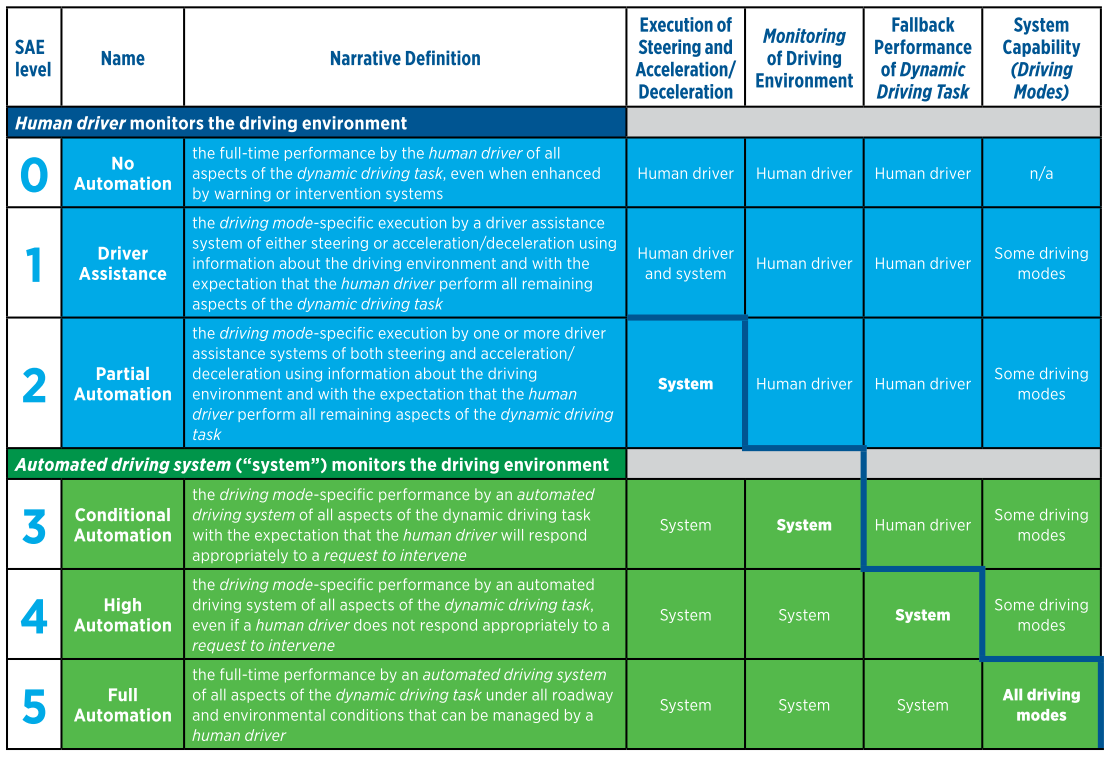
\includegraphics[width=1\textwidth]{fig/SAE}\hfill\
    \caption[SAE international automated driving levels]{SAE international automated driving levels. Figure from \cite{SAEinternational2016}}
    \label{fig:SAE}
\end{figure}

\section{Semi-Autonomous Vehicle Interfaces}
\subsection{Driver assistance technology}
A lot of assistance technologies, which are marketed differently by each automotive manufacturer, exist. A good visual overview is provided online\footnote{\url{http://mycardoeswhat.com/}}. Most assistance technologies try to increase safety. Only a few, such as automatic parallel parking, tackle convenience. As of now most of these systems work independently, in the future, these systems must work together to achieve full and semi-autonomous driving. For example, a vehicle could use obstacle detection in combination with pedestrian detection, lane keep assist, adaptive cruise control, and curve speed warning to drive autonomously; then use the drowsiness alert to detect if the driver still pays attention to the road during the self-driving time and finally use automatic emergency braking if the driver fails to intervene by himself. 

\subsection{Help the driver interfaces}
Before fully autonomous vehicles get deployed, the driver receives more assistance from the vehicles by assistance technology. There is technology that intervenes automatically and technology that just warns. For example, the vehicle could apply the brakes on its own if it detects a collision or it could play a warning sound. To help the driver there are both industry solutions, such as blind spot warning systems, and research papers from the HCI community:  \citet{Loecken2015} explored ambient light to warn of vehicles in the blind spot, \citet{Langlois2013} tested a prototype of a head-up display to communicate multiple messages from the driver assistance systems (Blind spot warning (BSW), lane departure warning (LDW), Forward Collision Warning (FCW)) by a peripheral display, \citet{Kim} and \citet{Langlois2016} tested augmented reality (in simulators) to make people aware of pedestrians and vehicles in dangerous scenarios. 
\citet{Larnaout2013} and \citet{Abdi} worked on the mapping of augmented overlays into the real scene. 

\subsection{Hand over of control}
For vehicles that are not yet fully autonomous but can drive autonomously in a few scenarios (SAE 2-3), the vehicle has to indicate when the driver needs to take back control. Humans stop actively driving the vehicle and start to monitor the autonomous system, unfortunately, research suggests that humans are not good at monitoring \citep{Naujoks2014TheConditions.}. It is difficult for humans to pay attention to tedious tasks for a long time. Moreover, driver assistance systems can be experienced as a loss of control and competency as well as a feeling of being at the mercy of technology \citep{Eckoldt2012AnSystems}. Tesla vehicles, which already employ a few self-driving functionalities (Adaptive Cruise Control (ACC), Lane Keeping Systems (LKS), Auto Lane Change (ALS)), make a rapid beep noise when the driver needs to take over control. However, two Tesla drivers died already because of inattentiveness while having autopilot turned on\footnote{\url{https://www.bloomberg.com/news/articles/2018-03-31/tesla-says-driver-s-hands-weren-t-on-wheel-at-time-of-accident}} and another one was caught sleeping\footnote{\url{https://www.theverge.com/2018/4/29/17298750/tesla-autopilot-british-driver-charged-driving-sleeping}}. Normally, the driver needs to touch the wheel to keep Autopilot active, however there are dangerous modifications sold that keep Autopilot steadily turned on\footnote{\url{https://www.autopilotbuddy.com/}}. These issues are still a field of active research. \citet{Politis} found that multimodal warnings are superior to unimodal warnings and reduce take over time, \citet{Merat2014TransitionVehicle} found that take over times are shorter when the vehicle requests them more regularly, and \citet{Koo2015} found preference for messages that describe why an event happened over how it was addressed (e.g. “Obstacle ahead” vs. “Emergency braking”).  \citet{Walch2017} give an extensive overview over current hand-over and collaboration strategies, they highlight in particular the importance of multimodality, adaptation of the system to the driver and conclude that the driver and vehicle should work as a team. \citet{Meschtscherjakova} dive into the issue that more automation means inferior driving skills. \citet{Rodel} suggest that trust in semi-autonomous vehicles (SAE-3) will be the lowest among the different automation levels because hand-over scenarios are not likely to be satisfactorily solved. 



\subsection{Ambient displays}\label{ssec:ambient}
Multiple approaches to make use of peripheral sight displays in cars exist. The most popular are Head-Up-Displays, which were originally developed for military aircraft. Other approaches use lower resolution light displays: To support lane change decisions \citet{Loecken2015} and \citeyearpar{Locken2015} used an LED strip to show information in peripheral vision. They argue that such a type of display can be used to inform drivers continuously without distracting them. A similar approach was followed \citet{Meschtscherjakov2015} to inform drivers about their current speed and to help them maintain it; \citet{Matviienko2016} used LED light to show drivers navigation information such as when to take turns; \citet{Hipp2016} integrated light into the back of the vehicle to support reverse parking maneuvers. These examples transport information into peripheral sight to solve issues of dual-task interference \citep{Wickens2002}. Ambient displays are a type of calm interfaces\footnote{\url{http://www.ubiq.com/hypertext/weiser/calmtech/calmtech.htm}} that should make information visible at a glance. \begin{quotation}{\emph{In Ambient Displays information is moved off the screen into the physical environment, manifesting itself as subtle changes in form, movement, sound, color, smell, temperature, or light. Ambient displays are well suited as a means to keep users aware of people or general states of large systems, like network traffic and weather.}} \citep{Pousman2006} \end{quotation}  Because ambient displays are meant to be unobtrusive it is difficult to evaluate them with traditional User Interface Heuristics that focus on systems with clearly defined tasks such as productivity and efficiency. A new heuristic to evaluate such displays was presented by \citet{{Mankoff2003}}. Generally, ambient displays are important to a user’s sense of well being and general awareness, but not critical to their work or personal life \citep{Pousman2006}. Contrary to traditional interfaces, before people can use ambient displays they need to understand \emph{that} information is visualized, \emph{what} kind of information is shown and \emph{how} it is visualized. 
%\citet{Holmquist2004} and \citet{Gridling} performed an ethnographic study on collaboration between co-driver and driver.    

\subsection{Interface Concepts}
\emph{Gamification} is the application of game design elements and game principles (such as points, badges, and leaderboards) in non-game contexts.
The authors \cite{Schroeter2016} created an AR game for semi-autonomous vehicles to increase the attentiveness to the road and increase situational awareness. \cite{Rodriguez2014} created an ambient display for the use of gamification to challenges players to avoid unsafe driving behaviors.  In \cite{Schroeter} the authors find that one of the major causes of accidents among young drivers is boredom and distraction by smartphones. They suggest that Gamification might keep young drivers engaged. Even though these concepts are relatively simple, Gamification might be a valuable tool to keep drivers engaged with their semi-autonomous vehicles. For fully autonomous vehicles gamification does not appear to be a necessity as passengers can stay engaged with whatever entertainment they like. 

\emph{Vehicle interfaces concepts for passengers} are very rare compared to driver interfaces: In a simulator study the gaze of the co-driver was visualized for the driver to inform of demanding driving situations \citet{Trosterer}, for travel groups that are spread amongst multiple vehicles \citet{Knobel2012} explored interfaces that created relatedness between them, \cite{Wilfinger2011} explored interfaces for children in the backseat and \citet{Hakkila2014} developed a concept for a mixed reality passenger window. 

\section{Fully Autonomous Vehicle Interfaces}\label{sec:interfaces}
Published research on interfaces for autonomous vehicles is sparse. 
\begin{figure}
    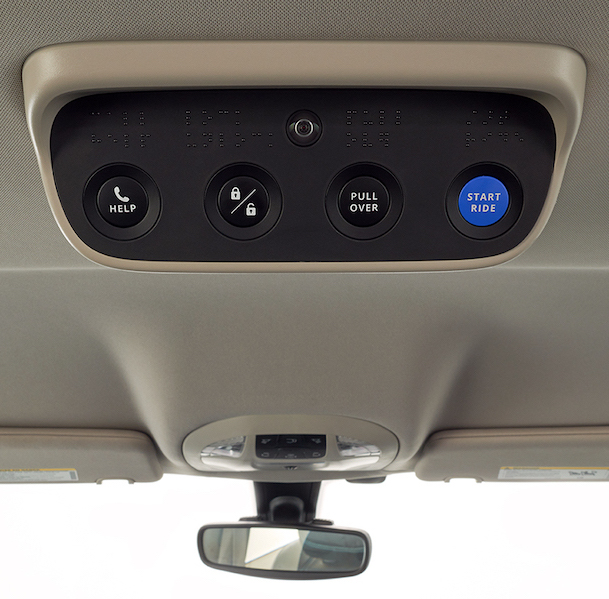
\includegraphics[height=0.27\textwidth]{fig/WaymoButtons}\hfill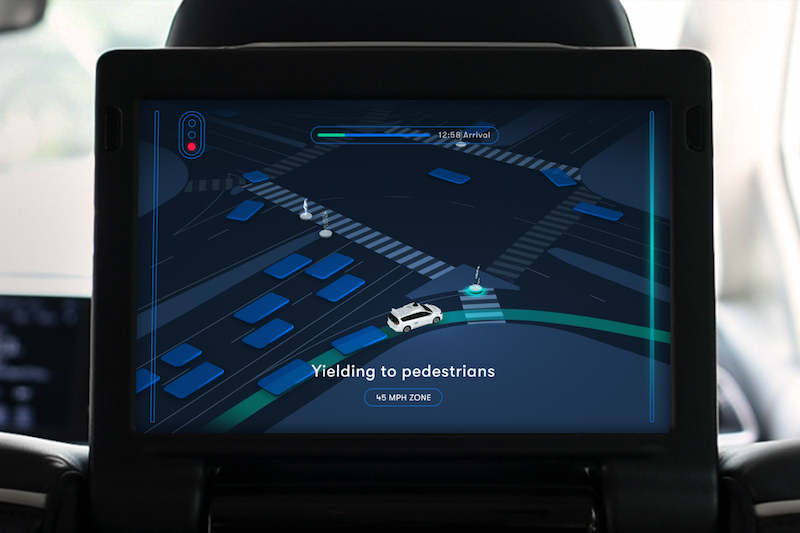
\includegraphics[height=0.27\textwidth]{fig/WaymoScreen}\hfill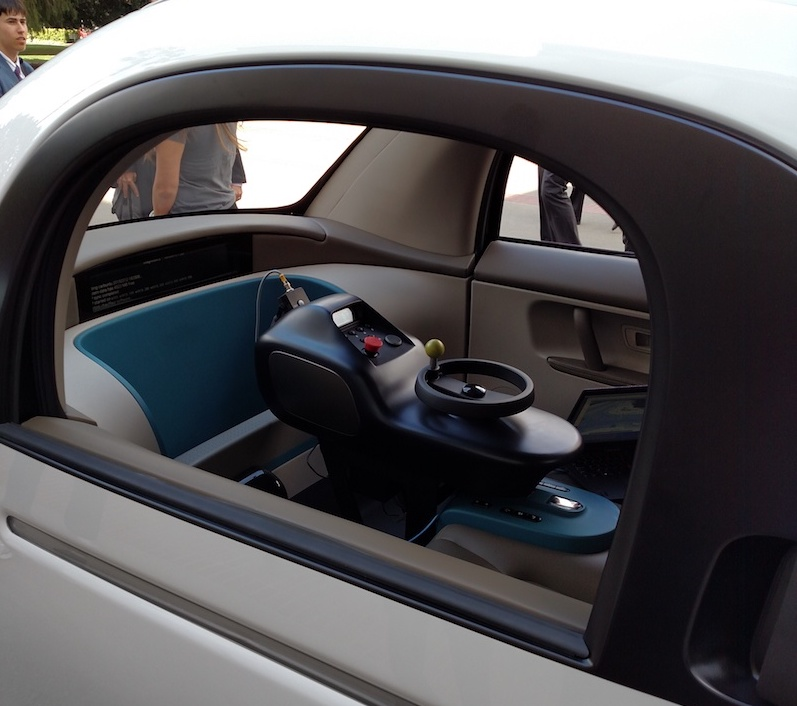
\includegraphics[height=0.27\textwidth]{fig/GoogleCar}
    \caption[Waymo autonomous vehicle interfaces]{Waymo autonomous vehicle interfaces. Images downloaded from: \url{https://arstechnica.com/cars/2017/11/fully-driverless-cars-are-here/} and \url{https://nathanpfry.com/google-self-driving-car-powered-by-carbuntu/}}
    \label{fig:fig-waymo}
\end{figure}
The vehicle interface of Waymo, the leading autonomous vehicle research company (by million autonomously driven miles), is very minimalistic. It has four buttons with braille text, a video camera and a display. The display seems to be without any touch input, the display is only used to show the route, what the vehicle detects and other sensor data (\emph{\fullref{fig:fig-waymo}, center}). The buttons allow to start the ride, pull over, lock/unlock doors and call for help (\emph{\autoref{fig:fig-waymo}, left}). The tour is planned and the vehicle is summoned by an accompanying app. 
Pictures from the older Google Car (now Waymo) show a very different interface (\emph{\autoref{fig:fig-waymo}, right}). 
It has a big stop button, a display below the windshield, a small display in front of the operation buttons and a horizontal steering wheel. Even if this interface might just be used for testing, it makes it very obvious how the newer Waymo interface tries to make driving autonomously look like nothing extraordinary. 

If we relate autonomous driving to using a cab, the software interface might look strikingly similar to those of ride-hailing services. Uber, Lyft, Mytaxi all use a map, which shows close by cabs. Furthermore, they make the user select the destination and starting point and allow to select a price category of vehicles.  

\subsection{Concept Cars}
\label{sec:conceptcars}
\begin{figure}
    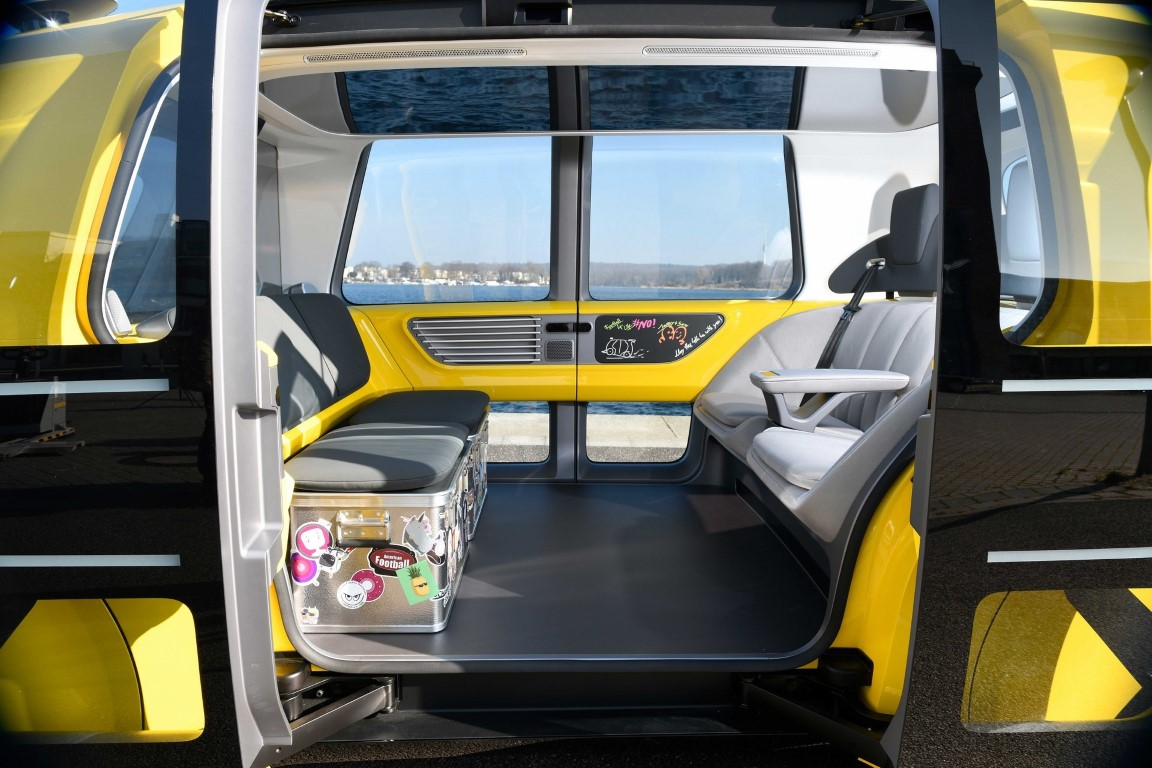
\includegraphics[height=0.2725\textwidth]{fig/school_bus_Mittel.jpg}\hfill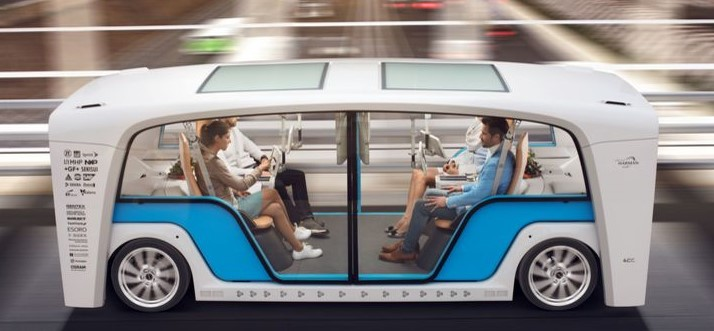
\includegraphics[height=0.2725\textwidth]{fig/snap.jpg}\newline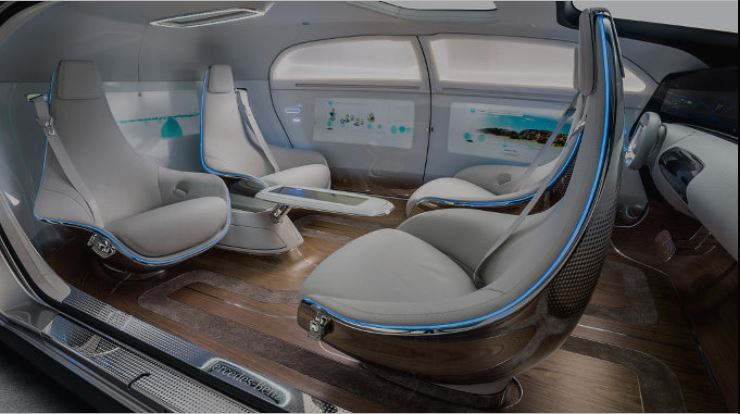
\includegraphics[height=0.28\textwidth]{fig/mercedes.JPG}\hfill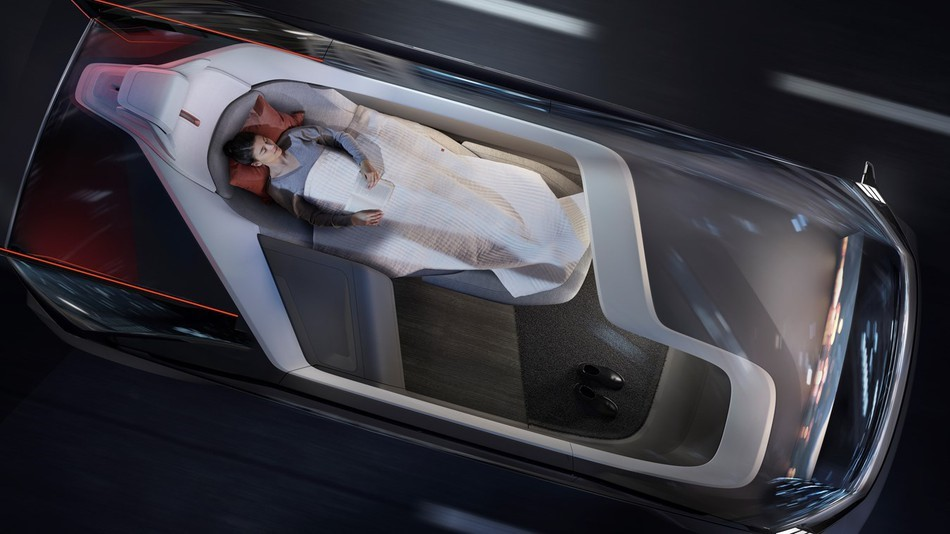
\includegraphics[height=0.28\textwidth]{fig/360c_Mittel.jpg}
    \caption[Concept Cars]{Concept cars: Sedric Schoolbus, Snap, F 015, 360c Downloaded from: \url{https://www.mercedes-benz.com/en/mercedes-benz/innovation/research-vehicle-f-015-luxury-in-motion/}, \url{discover-sedric.com/}, \url{https://www.rinspeed.eu/de/CES-Las-Vegas-2018_17_aktuelles.html} and \url{https://www.aircraftinteriorsinternational.com/news/passenger-experience/could-volvo-disrupt-domestic-air-travel.html}}
    \label{fig:conceptcars}
\end{figure}
Vehicles and vehicle concept such as the IBM Watson Olli, Volkswagen Group Sedric, Rinspeed Snap, Toyota e-Palette and Navya Autonom Shuttle show a public transport oriented design with minimalist interior and fixed simple seats. This is in stark contrast to the interfaces of personal autonomous vehicles such as the Tesla Models, Volvo Concept 6 or Mercedes-Benz F 015, cars that still have the steering wheel, dashboard and comfortable car seats and allow to retract or reverse them. The Volvo Concept 360c even has space for a bed and promotes it as an alternative to flying in the first class (\emph{\fullref{fig:conceptcars}}).   

\subsection{Pedestrian interfaces}\label{ssec:pedestrian}
One of the bigger HCI questions that need to be solved is 'how do vehicles interact with pedestrians'. Most of these communications are simple things like: 'Go ahead, I noticed you'. However to communicate these messages body gestures are necessary, which vehicles do not have the modes for. Possibilities are virtual avatars that represent the driver with, text or voice.  A clever communication method is used by the Mercedes-Benz F105, which uses a laser to beam a representation of a zebra crossing on the ground. Virginia Tech and \cite{FordMotorCompany2017FordPeople} built a prototype of an autonomous vehicle that uses a light strip to communicate with pedestrians, i.e., at a zebra crossing. Lyft cabs use a colored light pod, the amp\footnote{\url{https://take.lyft.com/amp/}}, to show to travelers which car is the one they summoned. \cite{Mahadevan2018} specifically looked into the nonverbal cues that allow pedestrians to cross roads and developed prototypes for a vehicle and Segway robot. 

\subsubsection{Communication with other vehicles} 
Communication with other drivers needs to be handled by autonomous vehicles too. Whether it is who will pass a crossing first, when in doubt, or when to honk for bad driving behavior. Interestingly, even now the possibilities to communicate with other drivers are limited. Only the headlamp flashers, the horn and turn indicators exist beside face to face communication. The Mercedes-Benz F105 has another addition, an LED text panel on the back of the vehicle. They use it to communicate that the vehicle is in autonomous mode and therefore driving slower than usual, much like vehicles from driving schools use signs to remind other drivers to be mindful.  

\subsection{Transportation-as-a-Service}\label{ssec:TaaS}
Transportation-as-a-Service (or also Mobility-as-a-Service) describes a predicted shift from vehicle ownership to renting and sharing vehicles, especially in urban areas. Even though ridesharing and carpooling was very common in the 40s and again in the 80s and 90s (in the U.S.) it declined rapidly by the 90s \citep{Ferguson}. The major reason for this decline is cheaper gas prices after the oil crises. Furthermore, cheaper vehicle costs, more spread out suburban living and improved roadway systems are the reasons for the death of carpooling. 

In urban cities, the new trend of TaaS is manifesting with ride-sharing, e-hailing services, bike-sharing programs, as well as car-sharing, all of which are enabled by the internet. In particular, improved map services and journey planners are conditions that allow users of TaaS to plan their routes individually. These services are usually available as subscription services or are 'pay as you go'. An early concept of TaaS was described by \citet{Tschanz1996TheServices}. Fully autonomous vehicles will most likely be employed as TaaS; Waymo, Uber, Lyft, and others have announced that they are working on such services and have even shown functional prototypes\footnote{\url{https://stratechery.com/2016/google-uber-and-the-evolution-of-transportation-as-a-service/}}. If autonomous vehicles are enabling ride sharing with strangers, a major concern is how to match the users of such services. The advantages of TaaS are potentially enormous: 'less time driving yourself', fewer greenhouse gases and pollutants, less traffic congestion, more random social encounters, less money spend on vehicle and vehicle maintenance and less space needed for parking lots.
Furthermore, autonomous vehicles might lead to reduced stress, improved productivity and fewer accidents \citet{Fagnant2015PreparingRecommendations}. However, whether or not autonomous vehicles will lead to less congested roads, fewer greenhouse gases are highly controversial. The reason is that an increase of comfort by autonomous vehicles might actually lead to more use of them, which in turn means that more miles are traveled\footnote{\url{http://humantransit.org/2015/11/self-driving-cars-a-coming-congestion-disaster.html}}\fnsep\footnote{\url{https://www.citylab.com/transportation/2014/04/will-world-driverless-cars-be-heaven-or-hell/8784/}}\fnsep\footnote{\url{https://www.ptua.org.au/myths/robotcar/}}. A good overview on the potential benefits and problems can be found in \citet{Litman2014AutonomousPlanning}. 

\subsection{Steering wheel}\label{ssec:steering}
\begin{figure}
   \hfill\ 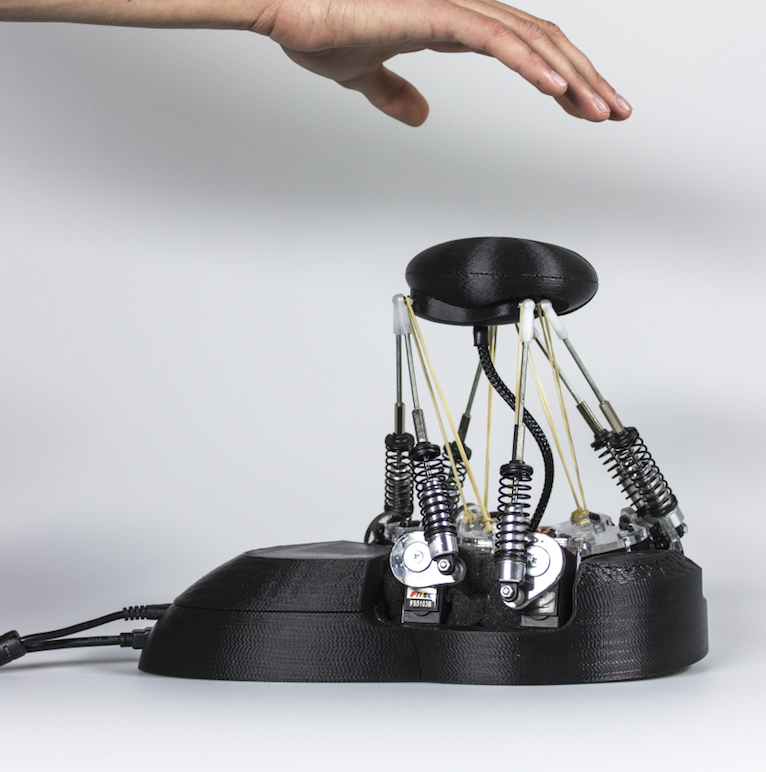
\includegraphics[width=0.4\textwidth]{fig/joystick}\hfill\
    \caption[The tactile joystick 'Stewart' for autonomous vehicles]{The tactile joystick 'Stewart' for autonomous vehicles. Image from \url{http://felixros.com/stewart.html}}
    \label{fig:joystick}
\end{figure}
Even the invention of fully electric steering, braking and pedaling, which allow the actual shape of these interfaces to be arbitrary, and the invention of assistance Systems such as autosteer and ACC did not change the general shape of the consumer driving interfaces at all. A well thought out tactile interface is that of industrial designer Felix Ross (\emph{\fullref{fig:joystick}}). It is a moving and vibrating joystick that mediates what the car is doing such as accelerating or taking turns. It is also meant to allow the driver to influence these decisions by moving the joystick. This control, however, seems more suited for self-owned autonomous vehicles where there is only one person that has order over it. In the TaaS concepts mentioned earlier, the steering wheels are left out. It might be worthwhile to explore collaborative driving interfaces further. 

\subsection{Car as a living space}\label{ssec:living}
If there is no driver in the vehicle, people could use the vehicle as their living room. This concept can be seen with car concepts that do not have seat belts anymore, are reversible or have a couch table in the center. An extreme version of this is the Hyundai Mobility Vision Concept \footnote{\url{https://www.hyundai.news/eu/technology/hyundai-motor-demonstrates-mobility-vision-with-hyper-connected-car-and-smart-house/}}, which presents a vehicle that docks physically into the living room and becomes a part of the interior. My preceding Intern  \citet{Honma2017SystemVehicles} concludes in his bachelor thesis work that there will be many different scenario dependent autonomous vehicles. For example, Disney branded vehicles that drive families to their parks or workout vehicles owned by gym chains that allow passengers to warm up before arriving at the gym. As discussed in \emph{\fullref{ssec:TaaS}} car ownership might become a thing of the past, the implication is that driving a car will become less about expressing an identity and more about “inhabiting a space” \citep{Laurier2012WhatCar}.

\subsection{Seating arrangements}\label{ssec:seating}
\begin{figure}
    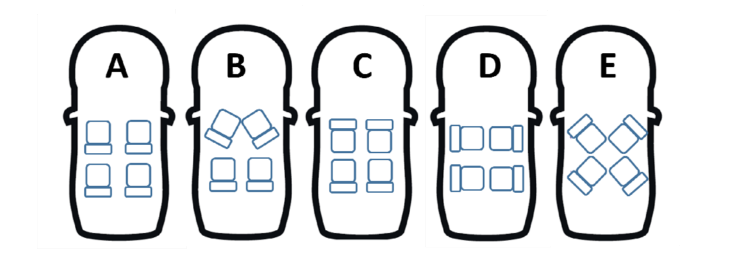
\includegraphics[width=1\textwidth]{fig/seating}\hfill\
    \caption[Seating arrangements]{Different seating arrangements in autonomous vehicles. Figure from \cite{Jorlov2017}}
    \label{fig:seating}
\end{figure}
A study of seating arrangements in autonomous vehicles from Navya\footnote{\url{http://navya.tech/en/autonom-en/autonom-cab/}}, Olli\footnote{\url{https://localmotors.com/meet-olli/}} and the Google Car reveals that they often do not have the traditional seating arrangement of consumer cars. Further concepts such as the Volvo Concept 26\footnote{\url{https://www.volvocars.com/de/modelle/concept-cars/concept-26}}, Mercedes-Benz F 015\footnote{\url{https://www.mercedes-benz.com/de/mercedes-benz/innovation/forschungsfahrzeug-f-015-luxury-in-motion/}}, or Volkswagen Group Sedric\footnote{\url{http://www.discover-sedric.com/en/}} show also very different seating arrangements.  \citet{Jungwirth2017LeadershipGroup} distinguish between autonomous vehicles for ownership, TaaS for People with Pods (vehicle for 2-6 people) or Shuttles (vehicles for more than six people) and TaaS for Goods with Urban and Highway use cases. In a qualitative study with 52 participants, \citet{Jorlov2017} explored future seating positions and activities in highly automated cars. In this study, the participants were seated on traditional chairs in front of an image of an autonomous vehicle and should imagine driving in such a vehicle. The \emph{\fullref{fig:seating}} shows the identified seating positions for longer drives with social activity. Users preferred the seating position C, followed by E and D. Even though this study is very limited in that it was conducted in a static setting and therefore no influencing factors such as car sickness or access to input devices were considered, it shows that autonomous vehicles might be a lot more dynamic in the seating arrangements.  

In highly autonomous vehicles it is not obvious who is in control and therefore not obvious where the major input and output devices will be. The ownership concepts such as Volvo Concept 26 sometimes keep the driver seat as the most important place. The steering wheel still exists, and cluster and entertainment displays are positioned to be easily accessible for the driver. The Mercedes F015 on the other hand places displays with touch input everywhere: in the cluster, in the side panels and inside of a central table. The central coffee table as a control device appears in other concepts too, such as the BOSCH CES 2015 car\footnote{\url{http://fearless-experience.com/index_neb.html}} or the Panasonic Autonomous Cabin Concept\footnote{\url{https://newatlas.com/panasonic-autonomous-cabin-concept/47280/}}. Autonomous vehicles that are more oriented towards the MaaS or public transportation often do not have any visible interfaces inside the cabin at all (See the Sedric, Olli and Renault EZ-GO\footnote{\url{https://www.renault.de/modellpalette/concept-car/ez-go-concept.html}} The Navya autonomous cab has one long vertical display such as can be found inside of subways. The control interface to summon such a vehicle is often a smartphone app instead. 

\subsection{Anthropomorphic features}
As vehicles become increasingly more intelligent and anthropomorphic, the question arises where the intellect and personality of the vehicle are located. Vehicles have an outside shell but contain the users inside them. It is well studied that vehicles are often seen as the extension of the driver's personality, that human facial features are recognized in the front end of automobiles and that people ascribe various personality traits to these \citep[see][]{Windhager2008FaceDesigns}. Some concepts of autonomous vehicles such as the Volkswagen Sedric and Smart Vision EQ Fortwo\footnote{\url{https://www.youtube.com/watch?v=fntak9UCnLs}} even animate their facial features. Vehicles of the premium range, as well as trucks and SUVs, often have masculine features as they portray speed, pleasure, control, risk-taking, and embodiment\footnote{\url{https://www.2025ad.com/latest/automated-driving-and-masculinity/}}. There is an interesting discussion by \citet{Balkmar2018} of whether autonomous vehicles might lead to a degendering and regendering of motor vehicles.
While the concept of the vehicle as a living space (\emph{\fullref{ssec:living}}) would indicate a process of deanthropomorphization, other studies point to the fact that people assign personalities and acknowledge autonomous vehicles’ humanlike intelligence \citep[see][]{Waytz2014}. An interesting thought is that because navigation system voices and other text to speech services are usually female\footnote{\url{http://www.bbc.com/autos/story/20160303-are-you-gps-gender-biased}}, would that mean that other anthropomorphic features of an autonomous vehicle have to be female as well? 

Some movies envision autonomous vehicles with a virtual cab driver (\emph{\fullref{sec:history}}). The Chinese car startup NIO has a digital assistant with simplistic facial features integrated into the console that can talk, blink and move its head. Nissan was experimenting in 2005 with a similar driving assistant (see \emph{\fullref{fig:robots}}). In a text by \citet{Perchonok2009FacilitatingLiterature} social interaction through speech and nonverbal communication with driver assistant robots are discussed. Other possibilities for visually present assistants are avatars and holograms. 
\begin{figure}
    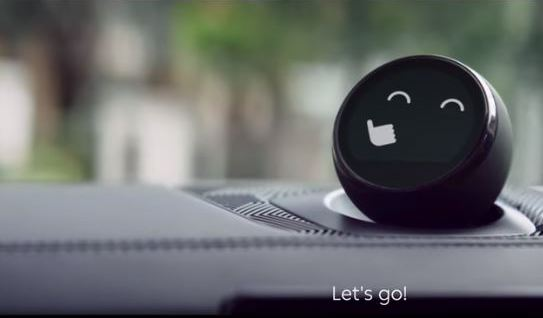
\includegraphics[height=0.28\textwidth]{fig/NOMI}\hfill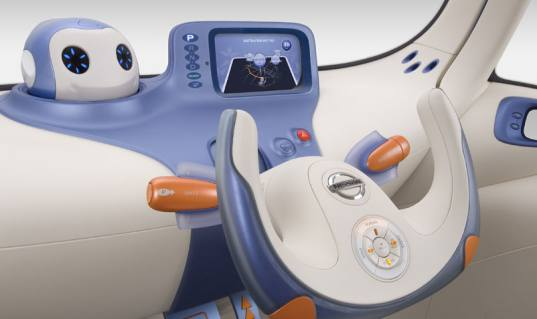
\includegraphics[height=0.28\textwidth]{fig/PIVO}
    \caption[Social Robots in Cars]{Social Robots in Cars. Left: NIO NOMI 
   Right: Nissan PIVO 2. Images downloaded from: \url{https://www.cleanthinking.de/nomi-so-sympathisch-kann-kuenstliche-intelligenz-im-auto-sein/} and adapted from \cite{Perchonok2009FacilitatingLiterature}.}
    \label{fig:robots}
\end{figure}

In my opinion there is not much use in a visually located  avatar; as of now it would suggest social intelligence, which assistants do not have yet; it would be difficult to be positioned in reach for all passengers, have issues with the uncanny valley and locate the perceived intelligence of the vehicle in one spot inside the cabin, whereas an autonomous vehicle appears as one intelligent agent on the outside. Instead, the inside of an autonomous vehicle might be compared metaphorically to a womb. A safe, comfortable place that encases the passengers and takes responsibility from them (see also \emph{\fullref{ssec:living}}). A personality and character could help autonomous vehicles to establish the initial trust people need for it to use, just as the first successful ATM had a character and voice too\footnote{\url{https://en.wikipedia.org/wiki/Tillie_the_All-Time_Teller}}.

\section{Trust Self-driving Vehicles}\label{sec:trust}
Most fatalities (94\%) on the road can be traced back to human error \citep[see][]{Singh2015CriticalSurvey}. Only a few accidents occur because of technical flaws. Therefore, the most dangerous aspect of being in a vehicle is the driving behavior. If a human hands over operation of the vehicle to an autonomous system he needs to trust that it performs the driving task equally well. 

A study by \citet{Hauslschmid2017} investigated if three different visualizations could enhance trust in autonomous driving: a chauffeur avatar, a world in miniature and a display of the vehicles indicator lights. These visualizations reacted to four different situations (turn, close objects, traffic lights, and danger) and were presented on a head-up display in a self-built driving simulator. As opposed to the researchers' hypothesis the subjects rated the world-in-miniature higher in trust than the anthropomorphic chauffeur avatar. They hypothesize that the miniature world conveys a stronger feeling of competence and is, therefore, more suitable to the technical system than a human-like visualization.

Contrary to this finding \citet{Waytz2014} found that anthropomorphism (as measured by the subjects impression of how smart the car was, how well it could feel what was happening around it, how well it could anticipate what was about to happen and how well it could plan a route) increased trust in the vehicle. Moreover, participants were more relaxed in an accident and blamed their vehicle and related entities less for an accident caused by another driver in the anthropomorphic condition. The anthropomorphic features given to the vehicle in this study were the name, gender, and voice. 
In a study by \cite{Korber2018}, participants were manipulated in their trust before a semi-autonomous simulator drive. People in the trust promoted group scanned the environment less, spent more time on a non-driving related task and were more likely to crash into an obstacle. 
A study by \citet{Beattie} found that participants in a car simulator study felt more in control when autonomous vehicles communicated their driving decisions by spatial sounds as opposed to no sound feedback. The sounds they used in this study were recordings from real vehicles (acceleration, braking, gear changing, clutch, indicator, and ignition). Research by \citet{Helldin2013PresentingDriving} suggests that too high levels of trust can lead to dangerous over-reliance on autonomous cars. The authors found that their UI, which communicates the certainty of the autonomous car allows passengers to calibrate trust in the system and react more safely. 

In an ethnographic study over six days \citet{Lee2016} summarize dimensions underlying trust but as the authors suggest: more importantly on distrust.  Findings of this ethnographic study are that all passengers participating in this study felt anxious when they were not adequately informed, especially about future actions. Also, unpredictable events, such as somebody running in front of the vehicle, were worrying to participants; participants felt irritated by the robotic movement of the steering wheel and mentioned that they might prefer not to be able to see it turning. Finally, participants were positively influenced by trust if they saw a purpose in autonomous vehicles or negatively influenced by social factors, such as taxi drivers who will lose their jobs because of automation. The authors summarize that in order to enrich driving experiences in automated cars, it would be essential to identify the factors that cause distrust and transform them into positive experiences rather than emphasizing trust factors. 

\subsubsection{Trust autonomous robots}
Vehicles that drive autonomously are a type of robots. It might be beneficial to apply research knowledge from human-robot interaction to autonomous vehicles. There is an argument that a shift from vehicles as tools towards vehicles as intelligent agents is happening \citep{Thill}. Since robots are difficult to compare, robotics researcher \cite{Steinfeld2006}, try to identify common metrics that allow comparison of social robots among different applications. For social robots, those are interaction characteristics, persuasiveness, trust, engagement, and compliance. 

\section{Study Autonomous Vehicles}\label{sec:studies}
Waymo, the most visible developer of autonomous vehicles, praises itself for designing autonomous vehicles not just to be inclusive but to be developed for the disabled preeminently \citep{Waymo2018DriverlessApplication}. Even though developers seem to focus already on the importance of the User Experience, there are no common guidelines or measures for evaluating autonomous vehicles. In \emph{\fullref{ssec:living}} the idea of the vehicle as a living room was established and in \emph{\fullref{sec:trust}} trust was discussed; therefore the two most important emotional measures of an autonomous vehicle may be trust and comfort.  

A big issue is the lack of access to autonomous vehicles, especially fully autonomous vehicles of SAE 3 and up. Most autonomous vehicles employ a whole range of sensors and especially LIDAR sensors are still expensive\footnote{\url{http://www.latimes.com/business/la-fi-hy-ouster-lidar-20171211-htmlstory.html}}. Even at companies such as BOSCH, which do have autonomous vehicles, access to them is restricted as they are almost nonstop in use for testing by the self-driving vehicle groups. Even if researchers can get access to an autonomous vehicle, most likely it is only borrowed for a short amount of time, and therefore complex modifications of the vehicle or implementation of prototypes into the vehicles are difficult. Then, most states only issue licenses that require a safety driver and occupants to be employed by the autonomous vehicle manufacturer \citep[see][]{Jones2013AutonomousReport}. 

Therefore, studies of autonomous vehicles often use lower level autonomous vehicles or are of short duration. 
Most published user research in vehicle interaction uses car simulators as they allow for highly controlled experiments, which are needed for experiments with internal validity. To increase the external validity of simulators some of them are paying extreme attention to details. For example, the interior of the vehicle is as close as possible to those of real vehicles and multiple sensors, speakers, projectors, and actuators replicate effects that occur during rides. These simulators proofed to be valuable for studies that focus on many aspects while driving, such as safety: i.e., it allows to measure reaction times accurately. 

However, a lot of important aspects of user research in autonomous vehicles cannot be recreated in simulators. Loss of control and lack of trust in the autonomous system are inhibitors (see \emph{\fullref{sec:trust}}) against the use of autonomous vehicles, it is difficult, if not impossible to recreate these aspects in simulators. Once test subjects enter a simulator, they know that they are part of a controlled experiment and if a simulated accident occurs, it would not be of any harm. Consequently, immersion and presence are lost. Perception of danger and immersion are lower, and moreover, sleepiness is higher in a simulator than in a real car \citep{Hallvig2013}.
Simulators are optimized to recreate the experience of driving, which means that the driving inputs such as steering and braking are simulated well. Even though some simulators have moving cabins, the inertial and vestibular cues, which are needed for distance perception are weakly recreated. Evaluating perception in driving simulation experiment, are challenging to recreate closely. Passengers are usually not researched, and therefore, most driving simulators do not even have back seats (see \emph{\fullref{fig:simulators}}). To sum up, simulators study often suffer from ecological validity, which might negatively influence the external validity of experiments. 

\subsection{On the road driving simulators}\label{ssec:simulator}
\begin{figure}
    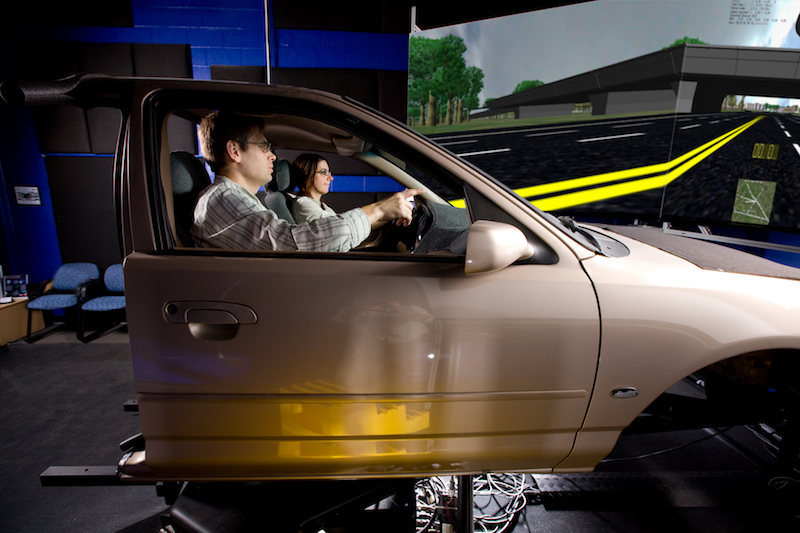
\includegraphics[height=0.3\textwidth]{fig/simulator}\hfill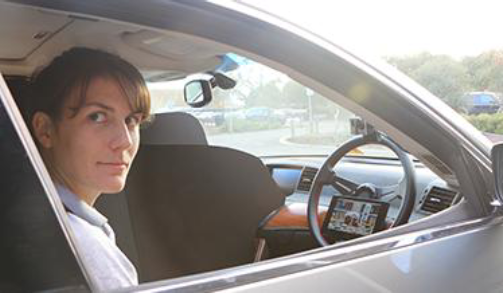
\includegraphics[height=0.3\textwidth]{fig/rrads}
    \caption[Driving simulators]{Left: Driving simulator of the University at Buffalo. 
   Right: The Real Road Autonomous Driving Simulator. Images downloaded from: \url{http://www.buffalo.edu/news/releases/2008/12/9819.html} and adapted from \citet{Baltodano2015}}
    \label{fig:simulators}
\end{figure}
Interesting approaches of on the road \emph{Wizard of Oz} experiments have sprung up recently.  WOz studies are sometimes criticized for their validity and use of deception\citep[see][]{Riek2012WizardGuidelines}. However, testing the user experience of real humans in close to real-world scenarios is often not possible otherwise. 

The Real Road Autonomous Driving Simulator by\citet{Baltodano2015} uses a partition to separate the test subject on the front passenger seat from the actual driver (see \emph{\fullref{fig:simulators}}). Even though the researchers do not use overt deception, some participants believed that they were riding in a real autonomous vehicle. This platform allows to test prototypes quickly and might be very effective to study handover scenarios. Indeed a similar system was developed to test exactly such scenarios: Marionette by \citet{Wang2017} is specifically designed to allow the test of semi-autonomous systems. It uses a right-handed driving vehicle so that participants can sit in the left seat, which is in most countries the driver's seat. Furthermore, it uses a gamer driving wheel for feedback but also a possibility of intervention. If the test subject steers accelerate or brakes with the gaming wheel or pedals, LED signals show the driving wizard what the test subject is doing: e.g., steering left or braking. He can then recreate these driving decisions with the real driving controls. During the ride study participant as well as the context for each drive are recorded because of the variability between each participants test drive. 

Another interesting approach is VR-OOM by \citet{Goedicke2018}, an on-road VR driving simulator. The researchers make the test subjects sit in a real vehicle, which drives over an open area such as a parking lot. The vehicle is steered by a driving wizard and additionally controlled by another interaction wizard; the test subject wears a VR headset, has gaming steering wheels and pedals in front of him and sees a virtual car and road while feeling the actual motion of the vehicle. For this approach, the virtual and physical location of the vehicles is synchronized. This approach allows testing a few other use cases that might not be possible in another setting. Still, the size of the parking lot restricts this setup, longer driving studies are not possible. Subjects will stay aware that what they see is fake, which impairs the feeling of presence. 
To test the interaction of pedestrians with autonomous vehicles \citet{FordMotorCompany2017FordPeople} and \citet{Rothenbucher2016} covered the driver with a vehicle seat costume. This allows testing how pedestrians interact with vehicles as if there are no driver insights. 

\subsection{No eye contact}
These on the road Wizard of Oz experiments do not use overt deception but disconnect the test subject from the driver. I argue that for testing human-machine interaction with autonomous vehicles it is important that the test subjects feel that they are on their own. If they see that there is another researcher (e.g., the interaction wizard) in the vehicle they might already have an initial trust in the whole autonomous system right from the start. If they can make eye contact with a researcher, they might establish empathy with the researcher \citep[see][]{Haase1972NonverbalCommunication}, and this could overshadow the trust of the test subject into the system. If there were any inconvenient or dangerous situations, they could always rely on them, a person with competence, as a backup. Therefore, it is important that the test subject can neither establish eye contact with a researcher in the vehicle nor a driver. We know that taxi drivers employ multiple strategies to build trust with their customers \citep[see][]{Gambetta2005Streetwise} and we are interested in the trust of the test subject into the “autonomous system” not of that into the researcher. Furthermore, some passengers show “back-seat driver” behavior if they are not driving themselves\footnote{\url{https://www.psychologytoday.com/us/articles/201005/field-guide-the-backseat-driver-pedal-the-meddle}}. It is important to investigate how this type of people feel if they are not in control of themselves and also cannot perceive how the vehicle is driving from gestures and sight of a human. 

\subsection{UX Factors}
\label{ssec:UXfactors}
The importance of the Users Experience in Interface Design has become acknowledged \citep{Soegaard2013TheEd.}. Some important measures of user experience in autonomous driving simulators were identified by \cite{Ive}. The following is an adaption for real road driving simulators: 

\begin{itemize*} 
  \item Trust in technology and automated systems\quad
  \item Plausibility of the (self) driving scenario\quad
  \item Car sickness\quad
  \item Comfort\quad
  \item Driver profiling\quad
  \item Need for control\quad
  \item Sensation seeking\quad
  \item Needs\quad
  \item Emotional response\quad
  \item Perceived quality\quad
\end{itemize*}

Compared to \cite{Ive} measures the following were changed: \emph{Measuring Presence in a Virtual Environment} is not required for real road driving simulators; however, the plausibility and convincingness of the wizard of oz setup are of importance. \emph{Simulator Sickness} won't occur in a real road driving simulator, however, car sickness does. For fully autonomous systems (without hand-over scenarios) \emph{sleepiness} is of lower importance though low alertness could indicate high trust in a vehicle. As argued in \emph{\fullref{sec:trust}} comfort might be of the most important UX factors for fully autonomous vehicles. Therefore, sleepiness was exchanged for comfort. To measure comfort or relaxation, possibly physiological measures can be taken into consideration. For example, the absence of stress indicates relaxation \citep{Salai2016}. \emph{Driver profiling} should focus not on the driving style (e.g., driver’s skill level) but on co-driver behavior (e.g., if passengers are used to be back-seat drivers). \cite{Burger1979TheControl} scale could measure the 'need for control' of an individual.

\subsection{Car sickness}
\label{ssec:carsickness}
One of the major selling points of autonomous vehicles for the average driver is the expectation that they can free up driving time for more valuable activities. However, car sickness is a strong inhibitor against that argument. Individuals' suffering from car sickness varies greatly but most people are not able to read books during drives. Motion sickness is most frequently caused by the conflict between visual and vestibular inputs; these critical conflicts will increase with improving image quality of onboard displays \citep{Diels2016}.

Further, loss of control over one’s movements and reduced ability to anticipate the direction of movement are also reasons for motion sickness \citep{Sivak2015}. The major car-sickness inducing movements are associated with horizontal accelerations caused by accelerating, braking, and cornering \citep{Diels2016}. These effects are more commonly experienced by passengers than the driver which explains why drivers suffer less often from car sickness. Narrow, opaque or small windows, non-forward gaze, and side or rear facing posture all worsen car sickness. Having the eyes closed, a supine posture and being asleep help \citep{Sivak2015}. Hence, the seating positions identified in \emph{\fullref{ssec:seating}} are possible causes of car sickness. 

People use various strategies against car sickness, one of the most important is to look out of the window regularly\footnote{\url{https://www.wikihow.com/Avoid-Nausea-when-Reading-in-the-Car}}, and to have the head higher up: \citet{Kuiper2018LookingCarsickness} used the MISC scale (by \citet{Bos2005MotionView}) and found that higher placed in car displays are beneficial against car sickness. In addition, motion sickness is related to the ability to anticipate the future motion path on the basis of motoric and visual information, which can also be provided via artificial enhancement of the visual scene: to measure air sickness in planes \cite{Feenstra2011AAirsickness} used MISC and JOSC self-reported measurement scales and showed that artificial moving visual images could be used to reduce motion sickness and thereby improve comfort.

\subsection{Data}
\label{sec:Data}
Self-driving vehicles need much data. Two of the most prominent companies have easy access to it: Tesla vehicles collect them from their customers while driving on the road and Google collects them from users of their Google Maps navigation software and also do they employ a huge array of mapping vehicles for their Maps service. An open source approach of data collection is used by comma.ai, a small company that sells OBD dongles that connect to the vehicle and a smartphone camera to connect driving data from their users \footnote{\url{https://medium.com/@comma_ai/a-panda-and-a-cabana-how-to-get-started-car-hacking-with-comma-ai-b5e46fae8646}}. While most data that autonomous car researchers are interested in is road data from LIDAR, radar and photo cameras, the steering, braking, and acceleration behavior of humans is also of interest. A naturalistic driving study by MIT goes even further \cite{Fridman2017MITAutomation} and collects additionally several data points which are of high interest for HCI research from the driver (video recordings of the cabin, interviews, and questionnaires). 

\section {The Best Interface is No Interface}
\label{sec:nointerface}
Golden \citeauthor{krishna2015best}'s book \emph{The Best Interface Is No Interface} \citeyear{krishna2015best}  provides an important line of thoughts. His major concern is that with the internet of things and smart homes devices that traditionally did a good job without any interface got “a screen slapped on it”. There is refrigerators, trash bins, microwaves that have big touch screens attached to them and often do nothing else with it then show time or weather. Even vehicles infotainment systems started to get problematic features such as checking Facebook or Twitter in the instrument cluster. Some new interfaces such as Amazon Alexa and Google Assistant do not even have a screen at all. For great experiences, designers need to consider the User Experience (\emph{\fullref{ssec:UXfactors}}). 
 
I agree that too many displays and input options inside vehicles are not just useless but also defy the purpose of great UX. Moreover, I do think that vehicle manufacturers should not try to compete with brought in devices. An iPhone or Nintendo Switch will always provide better entertainment than, e.g., a solitaire game embedded into a coffee table display developed by a car manufacturer. Instead, vehicle manufacturers and OEMs should focus on enabling these devices by providing enough power plugs, fast internet or a movie database from which passengers can stream movies. Ambient displays are a great example of interfaces without an interface (\emph{\fullref{ssec:ambient}}). 


\chapter{Ideation \& Specification}
\label{ch:ideation}
This chapter describes the ideation phase for a master thesis topic that aligns with the university's and Bosch Car Multimedia's interests' as well as my capabilities. The creative and brainstorming processes are guided by the Creative Technology design process \cite{Mader2014ATechnology}, which combines the concept of divergence and convergence with a cyclic concept. The chapter ends with the product specification.

\begin{figure}
    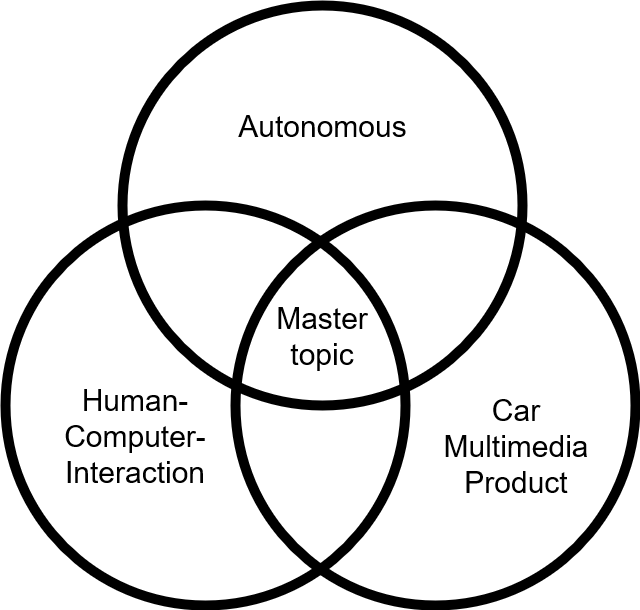
\includegraphics[height=0.4\textwidth]{fig/MasterTopic.png}
    \caption[Workshop]{The three topic ares for a master thesis topic}
    \label{fig:mastertopic}
\end{figure}

The University rejected the initial topic proposed by Robert Bosch Car Multimedia North America in Ann Arbour. The idea was to create a smell sensing device or algorithm that is capable of registering dirtiness in rental cars or autonomous vehicles. This topic hardly involves any interaction component or interaction design part. As Bosch did not have a topic alternative at hand, I developed the master topic on my own during the internship and worked on a few other tasks in parallel. The master topic should potentially result in a Car Multimedia Product, have a strong Human-Computer-Interaction component and should deal with autonomous vehicles (\emph{\fullref{fig:mastertopic}}). The Bosch Car Multimedia Division is currently making most of their money with infotainment systems, instrument clusters and head up displays. Infotainment Systems are the Software and Hardware that control the climate system, show the navigation system, control music, and radio or enable Apple CarPlay or Android Auto. The Instrument Cluster or head up displays show the speedometer, engine parameters, and navigation information. Fully autonomous vehicles, autonomous public vehicles, in particular, do not need any of these systems in their current form. In collaboration with an UX designer at Bosch, I discovered the frame of topics that would work for Bosch CM. Passenger to car interaction is of interest to Bosch Car Multimedia, but car to environment (pedestrians) interaction is not, as this would be the responsibility of another division. In the first steps, I created as many project ideas as possible and started to research if they were unique. I collected related works, concept ideas, used creative thinking methods and tinkering. Product ideas were sketched on paper, and a long topic list was compiled. 
\begin{figure}
    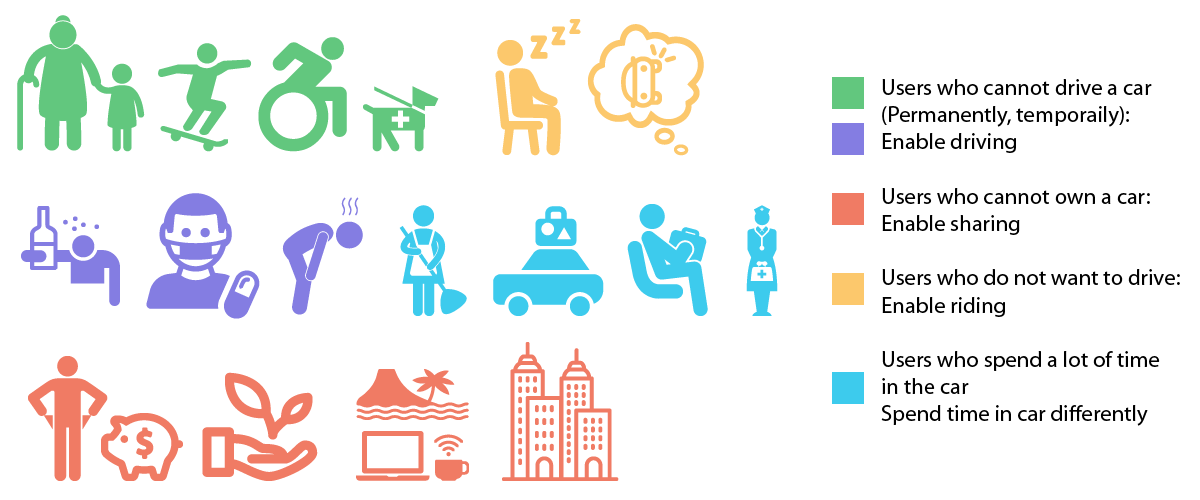
\includegraphics[width=1\textwidth]{fig/users.png}
    \caption[Users]{New user groups of autonomous vehicles: Elderly, young \& youth. Too sluggish \& too scared to drive. Drunk, sick \& tired. Workforce, travellers, commuters \& carers. Moneyless, savers, environmentally aware, nomads \& parking place restricted.}
    \label{fig:users}
\end{figure}

The seed for brainstorming was the newly reached user groups by autonomous vehicles (See  \emph{\fullref{fig:users}}) and the loss of human contact in cab scenarios. 

\emph{Cab driver tasks are:}
\begin{itemize*} 
  \item Clean \& maintain\quad
  \item Welcome (check tickets)\quad
  \item Help with luggage\quad
  \item Help with special needs\quad
  \item Plan route\quad
  \item Drive\quad
  \item Inform\quad
  \item Small-talk (personality)\quad
  \item Recommend (local)\quad
  \item Secure \& surveil (give trust)\quad
  \item Goodbye (pay)\quad
\end{itemize*}

Useful concepts for ideation were: Personalization \& context awareness, perceived intelligence of vehicle (personality and location of intelligence, possibility to express), shift from a ‘joy of driving’ to a ‘joy while driving’, living-room environment without using hands, cloud as a central hub where all information will pass through, shift from explicit to implicit interaction, discrepancy between public and private. Some HCI questions that need to be solved are: How can passengers feel that they are in control? How can passengers participate in driving decisions? How can the car talk, express and indicate? How does the car listen (direct \& passive)?

\begin{quotation}\emph{Starting with the user (blind, deaf, physical ability) to design an interior solution for autonomous cars during short duration (less than 15 minutes) commute. By basing this off the idea that if we design for a “disability” we, in turn, are designing for all. With your interactions with people who have different abilities you can uncover some of their needs and can redesign the interaction that this group has with a car. The solution could be voice, visual, or even haptic interactions. - Harsha, Bosch UX}\end{quotation}

In collaboration with the UX team, I turned these topic ideas into initial questions according to the Question Zero Concept from \cite{RobertBoschUX2017QuestionZero} and made sure that they align with the prioritization of activities (such as 'progressive vehicle interiors', NUIs and Mood Tech) according to the Bosch Mobility Trend Radar \cite{RobertBoschNA2017RegionalRegional}. 
Finally, the preferences of my supervisors at Bosch resulted in these topics:

    \begin{enumerate}
    \item Interior Communications through light.
    \item A system for an autonomous vehicle to communicate the driving decisions it takes to all passengers.
    \item Using voice as an interior control system.
    \item A product for visually or mentally impaired riders in autonomous vehicles that assures a sense of control when traveling alone.
    \item A system for passengers to gather trip information without the use of a driver.
    \item Other:
    \begin{itemize}
    \begin{sloppypar}
    \item A solution to reduce carsickness in autonomous vehicles.
     \item No located personal assistant but whole car interior as safe space (womb).
    \item Context-aware driving modes.
    \item Lowering distraction \& strengthening 
    the involvement of the driver through the use of V2V.
    \item Developing new usage scenarios/interactions for the BOSCH touch feedback system.
    \item A doorknob (window lifter etc.) which allows feeling in control in autonomous vehicles.
    \item Personality device (enable different car personalities for the use case, owner \& context).
    \end{sloppypar}
\end{itemize}
    \end{enumerate}

\section{Concept}
\label{sec:concept}
My personal interest is human-computer-interaction beyond screen-based interfaces. Concept cars from vehicle manufactures (\emph{\fullref{sec:conceptcars}}) rely heavily on large screens. Screens can be seen everywhere: In tables, windows, across the doors, behind the back seats, across the whole front and in the back of the seats. The best interface is no interface (\emph{\autoref{sec:nointerface}}). 

Almost in a 'flash of inspiration' the idea for the final product emerged: \emph{An indirectly illuminating LED bar that surrounds the whole cabin 360, and reaches all passengers with fluently distributed ambient information and mood lighting.} This light system should provide passengers with individual zone lightning that can be adjusted simply by touching it; enable the autonomous vehicles assistant to guide attention throughout the vehicle's cabin. Personal assistants such as Amazon Alexa and Google Assistant do not just rely on voice feedback but deepen the interaction through simple light feedback. This LED bar should be used to tell passengers crucial driving decisions the vehicle planned out and also allow it to communicate direction independently of the direction of travel: e.g., \say{Look over here for the empire state building}.
There is no driver to distract, therefore, brighter and more elaborate lightning can be used in cars. Fixed reading lights do not work with dynamic seating arrangements. Lightning can be used to calm or energize. Brought-ins (e.g., laptops, smartphones, game consoles and ebooks) will be the preferred entertainment and productivity tools over integrated infotainment systems. Car - passenger interaction is crucial, even if driving 'just works' without any interference by humans. 

\begin{figure}
    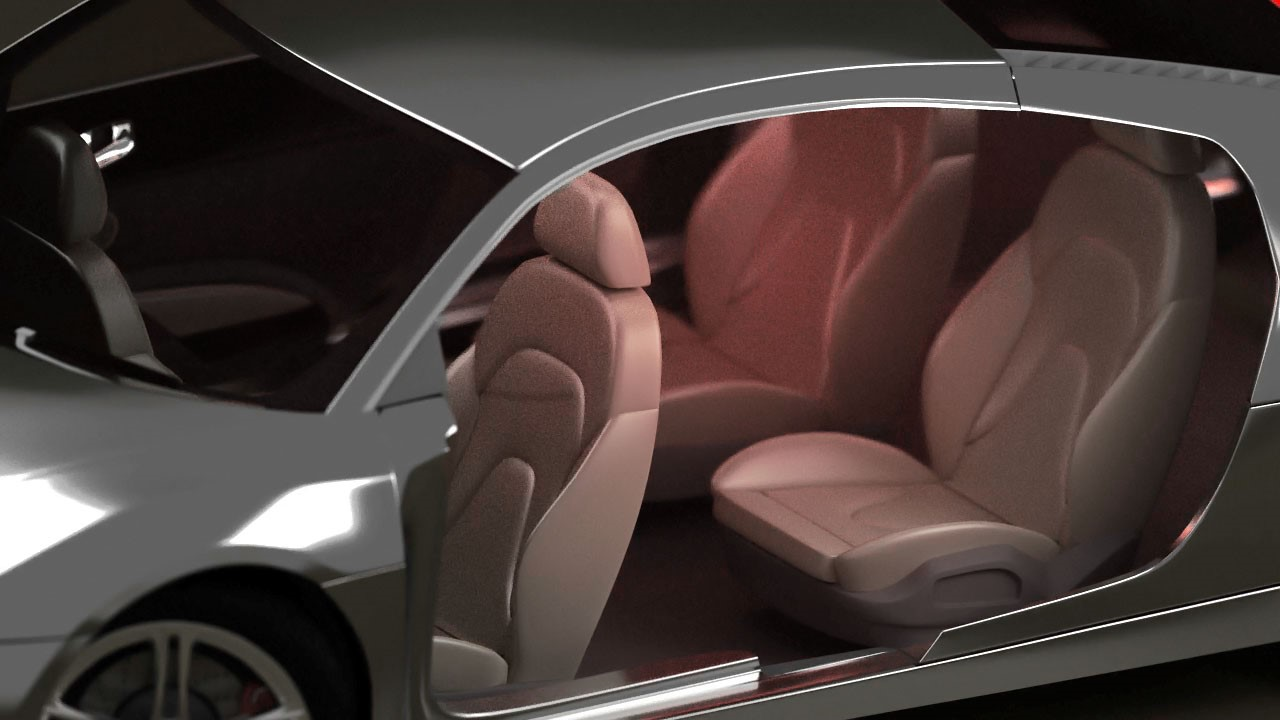
\includegraphics[height=0.28\textwidth]{fig/swerve_Mittel.jpg}\hfill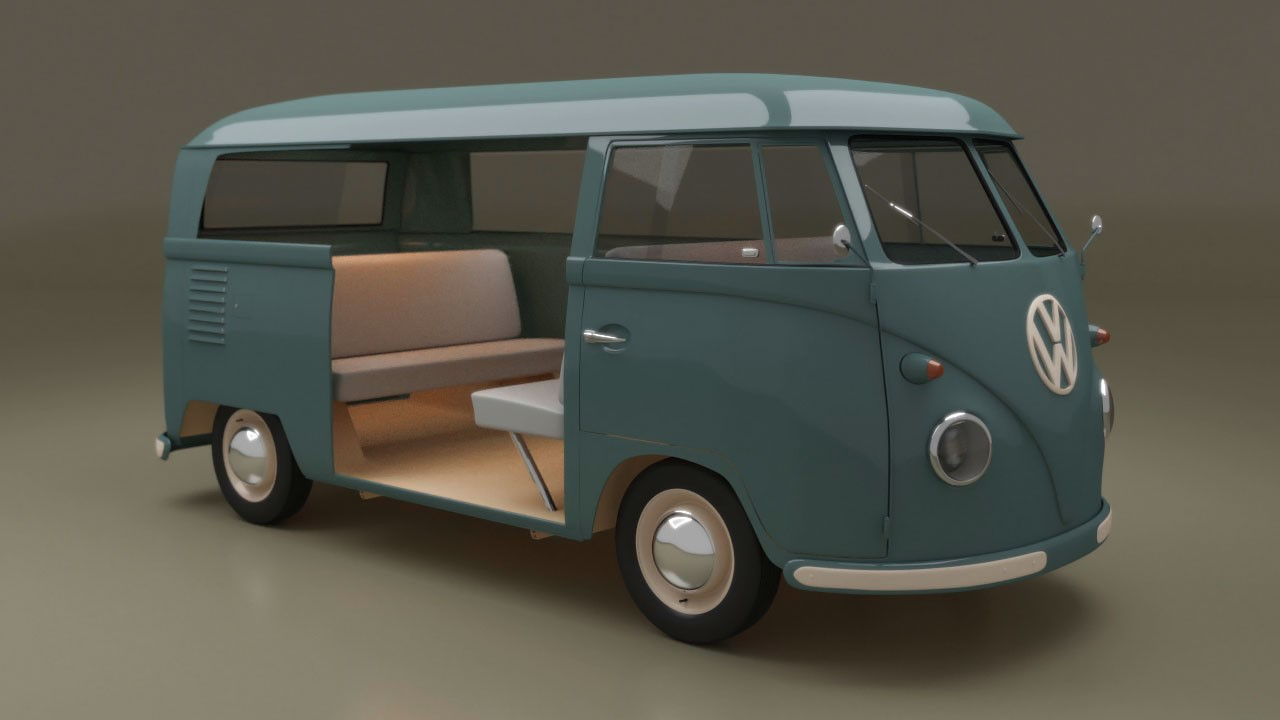
\includegraphics[height=0.28\textwidth]{fig/busLight_Mittel.jpg}\newline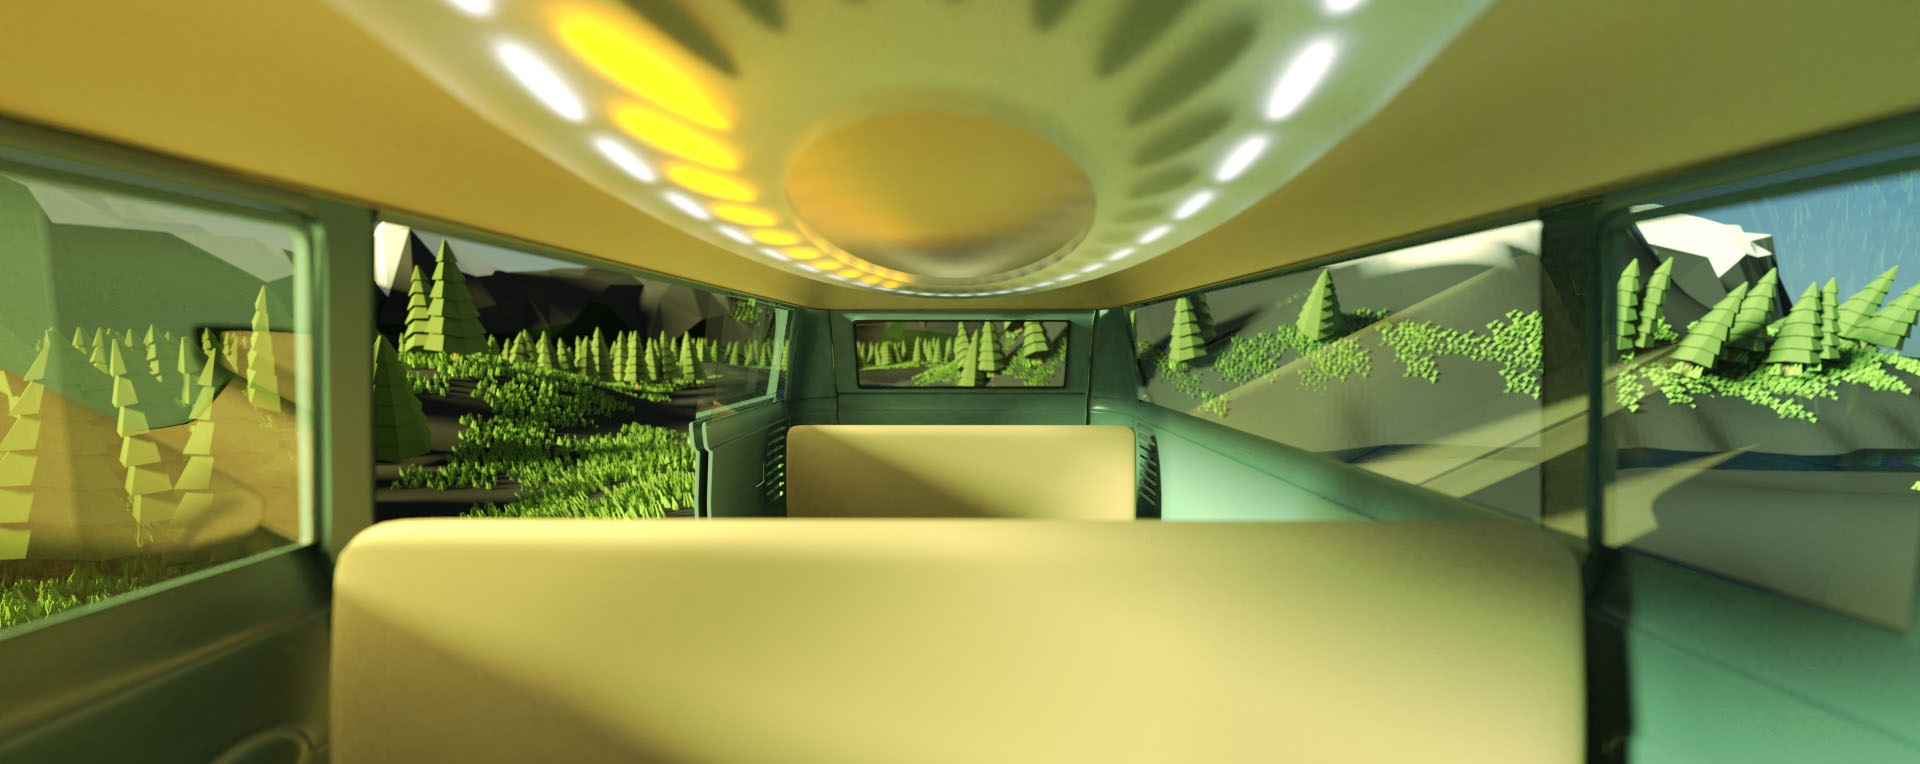
\includegraphics[width=1\textwidth]{fig/0013GRADIENTcut.jpg}
    \caption[Early Concept Render]{Early Concept Render: Swerve, Speed Up, Light Bar. (For animated versions check the digital appendix)}
    \label{fig:conceptrender}
\end{figure}

To convince supervisors of the potency of the concept and to try the feasibility of indirect lighting in vehicle cabins early on, looping GIF animations ( \emph{\fullref{fig:conceptrender}}) were rendered with the Blender Cycles renderer which provides global illumination through path tracing\footnote{\url{https://cglearn.codelight.eu/pub/computer-graphics/global-illumination}}. This allows visualizing indirect light and the light bounces inside the vehicle cabin. The 3D renderings use models that are licenced under creative commons license\footnote{\url{www.blendswap.com}: 1950's VW Van by Jay-Artist, Audi R8 V8 by Neubi, Mountain And River Low Poly by Hoboo}. The mood board in \emph{\autoref{fig:smoodboard}} contains visual and emotional inspiration for the project. It helps to set the atmosphere, communicate the idea of a finished product and the feelings it should provoke early on in the creative design process \cite{Cassidy2011TheTool}.

\begin{figure}
\centering
    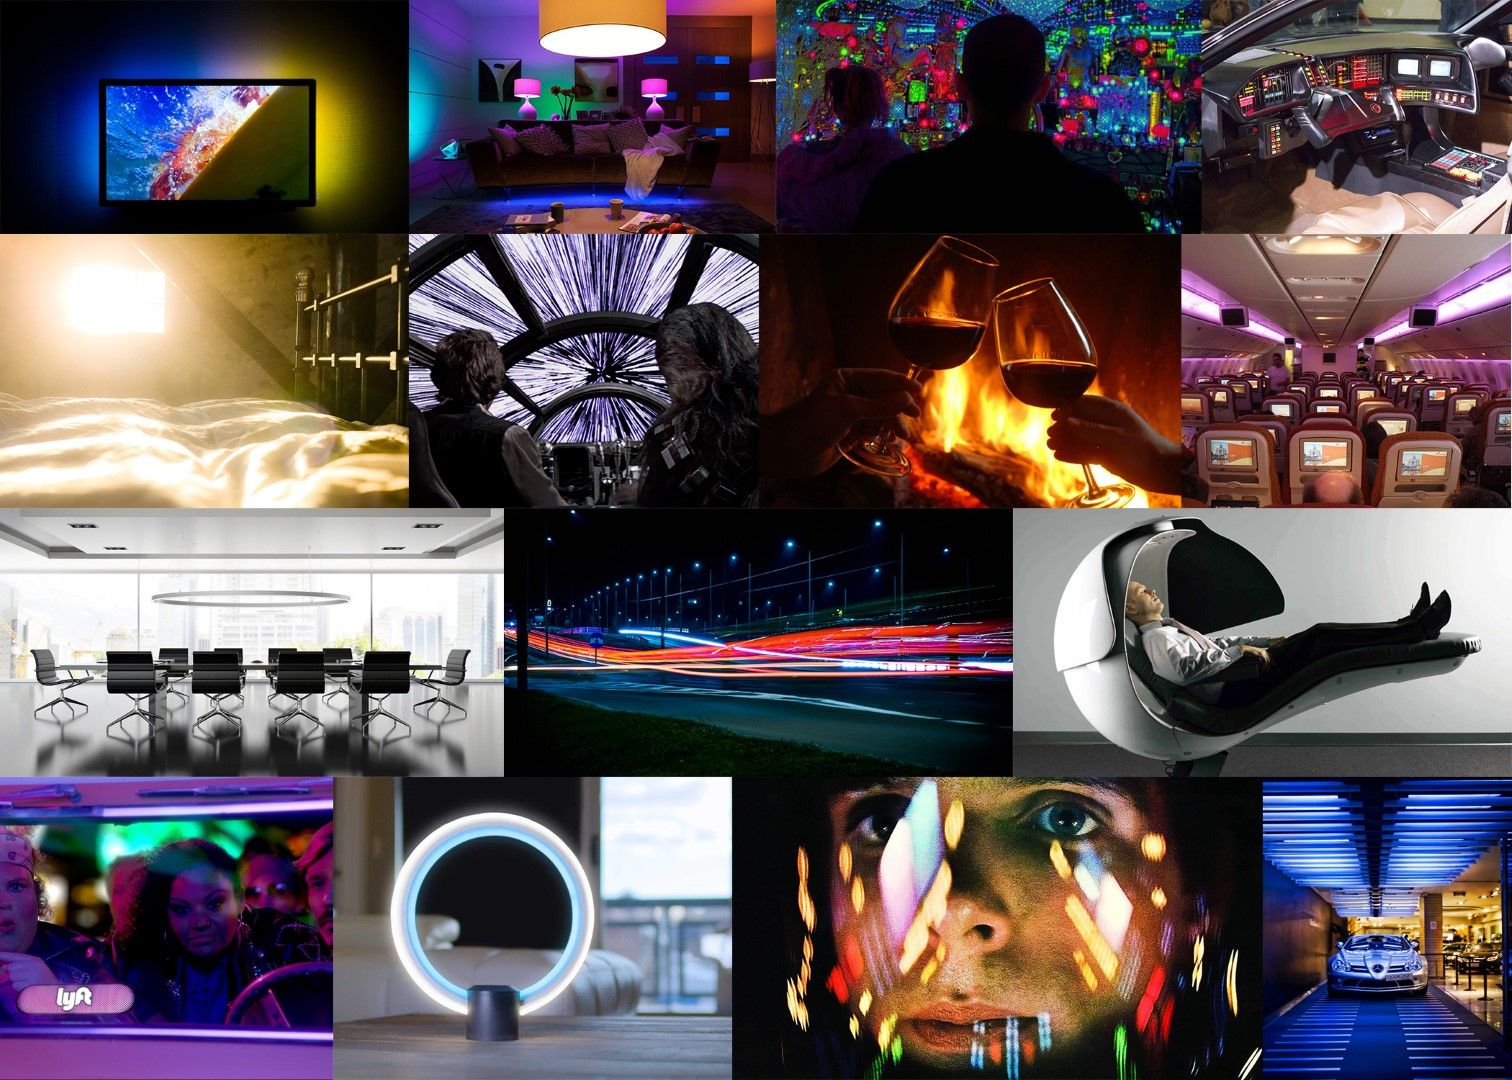
\includegraphics[width=1.\textwidth]{fig/moodboard_G.jpg}
    \caption[Moodboard]{Moodboard}
    \label{fig:smoodboard}
\end{figure}
\section{Light Animation Design}
\label{sec:Lightdesign}
In this section the design of light messages is discussed.

\subsection{Feedforward}
\label{ssec:feedforward}
Feedback in HCI is typically used to inform the user that the system is responding, to indicate progress or to confirm navigation. \citet{Djajadiningrat2002ButHow} state that feedforward, like feedback, returns information about the result of a process or activity. However, while feedback is communicated during or after the action, feedforward is information that is offered before the action takes place. Whereas feedback informs the user about the action that is carried out, feedforward informs the user about what the result of their action will be \citep{Vermeulen2013CrossingExecution}.

Feedforward is usually used in context with affordances of interfaces; here it is used as 'advance feedback before executing an action' \citep[see][]{Koo2015}. The automated machine provides this feedforward information irrespectively of user call for action. 
Feedforward is a new type of feedback that, in my opinion, should be provided by interactive automated systems to help humans understand their actions. 

\subsection{Message types}
The options for output in autonomous vehicles are almost endless. For multiple reasons, the users should not be overwhelmed with feedback from the vehicle. The low-resolution light display is limited by the number of different animations that can be displayed, the user cannot learn too many new messages at once and he might get annoyed by useless feedback. In a user study, we should only focus on a subset of messages to reduce complexity. Thereupon, it needs to be carefully curated what is considered important enough to be shown to the users.

In a driving context, it makes sense to distinguish between 'right now', 'soon' and 'planned long-term' information. ‘Right now’ is real-time information from the vehicle such as sensor data or outputs of the vehicle (driving). ‘Soon’ can be retrieved, e.g., from map data in the form of, e.g., calculated trajectories. Examples of planned long-term information are the route planning or traffic information. The light display might be best equipped to signal ‘right now’ and soon information because more complex future information is difficult to encode in such a ambient display and might be better suited for show through voice or displays. In the following scenarios that can be encoded by light animations are depicted. 

\subsubsection{Sudden driving behaviors}
Most of the sudden driving behaviors should only happen very rarely. Ideally, the autonomous vehicle is capable of foreseeing these scenarios early on and slow down smoothly. However, if they do happen the car should tell the passenger during these risky moves that it knows about the situation and is in control. Outside Vision is a light effect to show that other road users, who are driving recklessly, are noticed. (\emph{\fullref{fig:sudden}}). 
\begin{figure}
    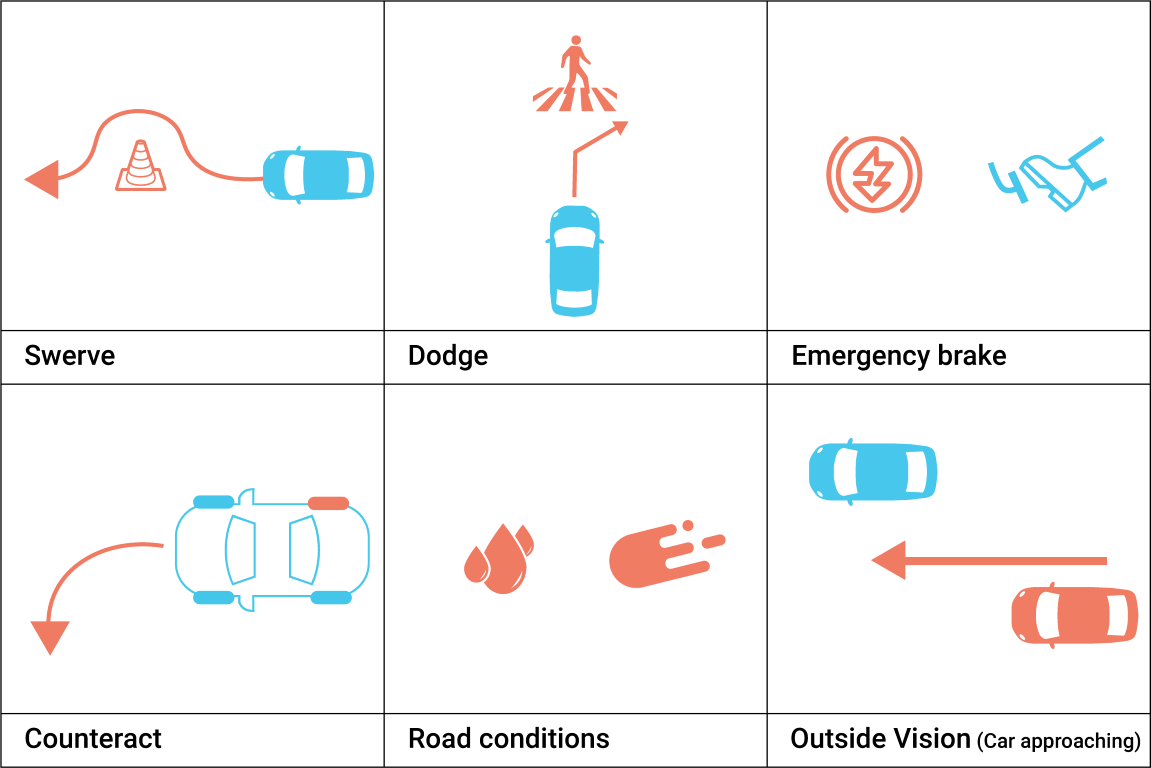
\includegraphics[width=1\textwidth]{fig/suddenmid.png}\hfill\
    \caption[Sudden Information]{Exemplary sudden information}
    \label{fig:sudden}
\end{figure}
\subsubsection{Planned}
Planned driving movements are most frequently shown. An autonomous vehicle or driver decides for these movements hundreds of times during driving. Even if the passengers can feel these movements with their body and deduce what the car is doing from how the street runs, the car should tell that is about to perform these actions. I hypothesize that the more noticeable these movements are, the more necessary it is to communicate them. Actions that are less frequent but deviate from the normal driving are more important to augment. (\emph{\fullref{fig:planned}}). 
\begin{figure}
    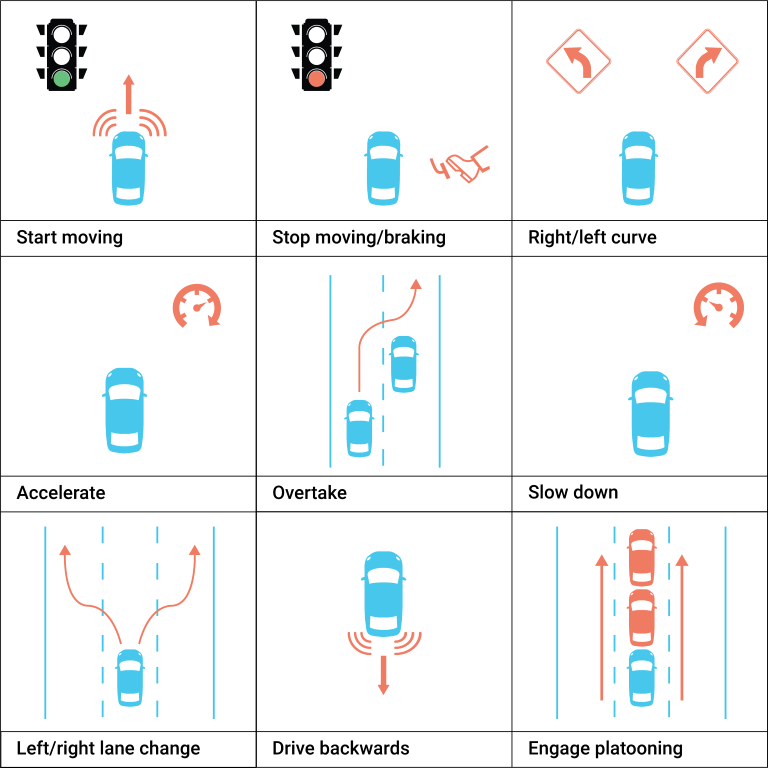
\includegraphics[width=1\textwidth]{fig/planned_1366.png}\hfill\
    \caption[Planned information]{Exemplary planned information}
    \label{fig:planned}
\end{figure}

\subsubsection{Route}
Route information is easily displayed through the navigation system of a car. Some of these pieces of information can be communicated actively by a light bar instead of passively by a display. Arrival time could be communicated by rising brightness; waking up the passengers and signaling that they have to become active again. Enter \& Exit can be animations that guide the passengers side of the car that it is safest to get off. Light signals can be used to draw attention to a specific direction. For example, a car could talk to the passengers about historical sights on the route and use light to show where to draw the attention (\emph{\fullref{fig:route}}). 
\begin{figure}
    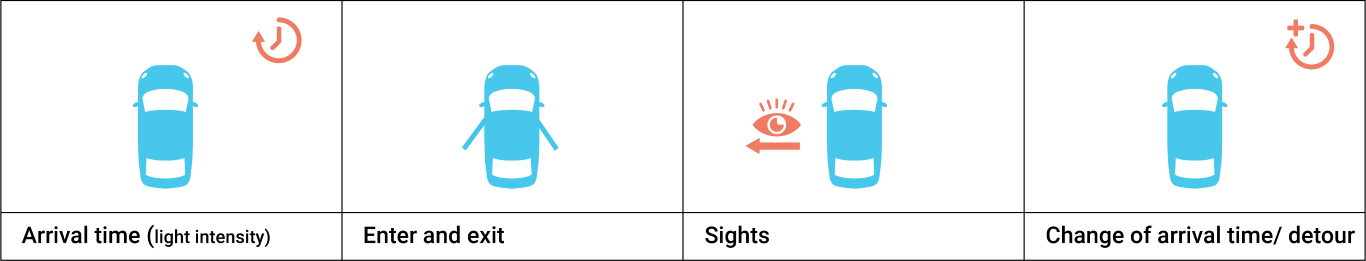
\includegraphics[width=1\textwidth]{fig/route.png}\hfill\
    \caption[Route information]{Exemplary route information}
    \label{fig:route}
\end{figure}

 In \emph{\fullref{fig:lightevents}} the messages are ordered by the underlying data and expected occurrence. Frequent events should be less notable, whereas exceptions must be strongly visible. States should not be too visible. Values can influence states and events but must not necessarily be visualized constantly. The subset of animations used in the final prototype was chosen according to their expected influence on driving comfort. 
 
\begin{figure}
    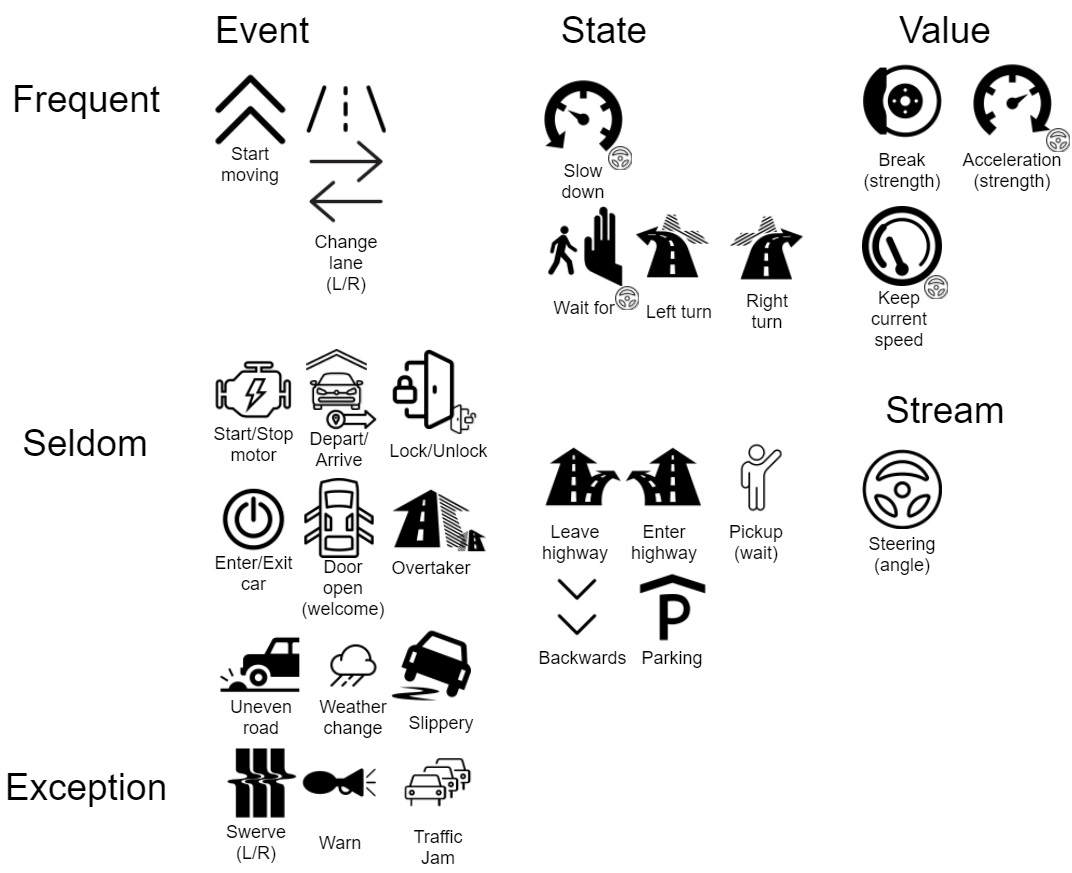
\includegraphics[width=\textwidth]{fig/tab-}
    \caption[Light Events]{Categorization of light messages by underling data}
    \label{fig:lightevents}
\end{figure}

\section{Animation behavior}
\begin{figure}
    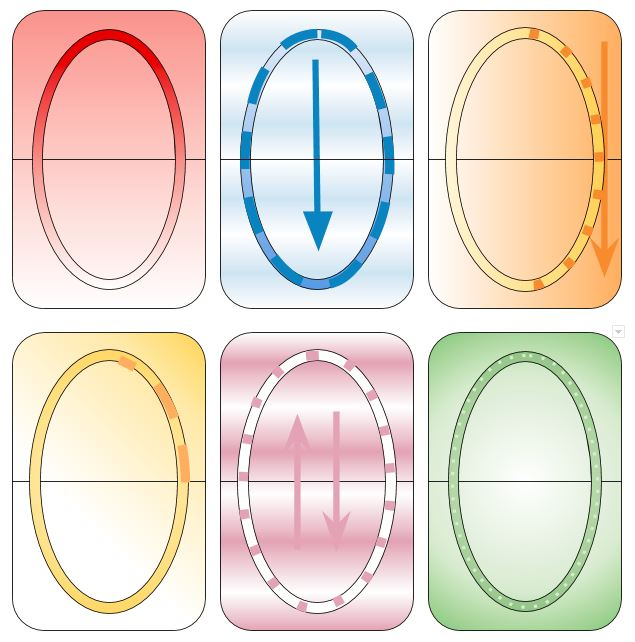
\includegraphics[width=0.6\textwidth]{fig/lightsignals.JPG}
    \caption[Light animations]{Graphical visualization of light animations. From top left to bottom right:
Brake (Hard), Accelerating, Into Right Lane, Right Turn, Uneven Road, Waiting}
    \label{fig:lightanimations}
\end{figure}
In \emph{\fullref{fig:lightanimations}} different ambient lighting animations are depicted. The arrows show the movement of animations, global 'fade in' and 'fade out' are not shown, the background gradients show how the car interior gets to light up. Brake and turn signal color coding is inspired by cues that the standard cars already give: red for brake lights and yellows for turn signals. This way signals that a car communicates to road users are projected inside the vehicle to passengers. Aggressive colors and colors that transport meaning by itself have to be used very carefully. Therefore, the red colors should not be too aggressive, e.g., for uneven road purple is used. 'Uneven road' uses forward and backward moving strips as a metaphor. A pulsating light depicts 'waiting' as if the car was in standby mode. Green could be interpreted as 'waiting for the green traffic light'. Accelerating is shown by fast moving blue lights, to give the impression of speed (See \emph{\fullref{fig:smoodboard}}).

\chapter{Realisation}
\label{Realisation}
\section{Light Display Shape}
\label{LEDshape}
As a first step possible shapes and places for the illumination were sketched on paper and then prototyped in full size with cardboard. The light should be visible in peripheral vision via reflections in the car interior. Thus, the placement needs to ensure that the light reaches the whole cabin, but does not obstruct the view. A cardboard ellipse with the width and height shown in Equation 3.1 filled average sized car cabins quite well. 
\begin{equation}2\pi \sqrt[]{\frac{\frac{113 cm}{2}^2 * \frac{140 cm}{2}^2}{2}}\approx 400cm \end{equation}
An ellipse is the ideal shape as it surrounds the passengers 360° and uses the maximal ceiling space without corners or bends.

\section{The human eye}
\label{sec:eye}
Some properties of the human eye and visual system need to be considered for the design of the ambient display. In  a book by \citet{Wordenweber2007AutomotiveVision} those that are relevant to the design of vehicle lighting (exterior and interior lighting) are presented. 
Lightness refers to perceived intensity of a color in relation to its illuminated context, whereas brightness refers to absolute achromatic brightness. Sometimes when the brightness of the ambient display is correct the term Lightness would be more exact. 

Human eyes can operate over a large range of brightness because humans do not perceive changes in light linearly but approximately logarithmic (Weber–Fechner law or Stevens's power law \citep[see][]{Brill2014DoesQuestion}). This has concrete effects on interface design and is often still unconsidered, for example the Android smartphone operating system switched the brightness slider just recently to logarithmic scaling to improve the user interaction\footnote{\url{https://www.androidpolice.com/2018/06/07/improved-logarithmic-brightness-slider-introduced-android-p-dp3/}}. 
\begin{figure}
    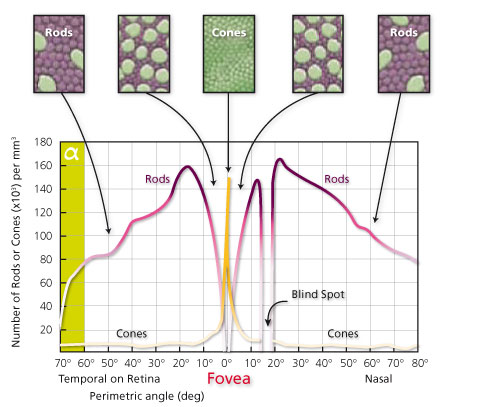
\includegraphics[width=0.8\textwidth]{fig/jjsDG.jpg}
    \caption[Distribution of Rods and Cones]{Distribution of Rods and Cones. Downloaded from: \url{www.sharp-sighted.org/index.php?option=com_content&task=view&id=58&Itemid=120}}
    \label{fig:eye}
\end{figure}
Cone cells, which are densely distributed in the center of the eye (the fovea), are more sensitive to colors, whereas rod cells, which are found concentrated in the periphery of the retina, are more sensitive in general but not to color (see \emph{\fullref{fig:eye}}). Further, red–green color (L-M channel) sensitivity declines more steeply toward the periphery than sensitivity to blue–yellow  (S-(L + M) channel) colors \citep{Hansen2009ColorField}. How humans perceive color in their peripheral is still debated: some researchers claim that L-M cone opponent vision is absent in peripheral vision (>25degree), whereas others showed that with a large target size and a low temporal frequency (1 Hz) different hues would be perceivable up to 90 degree. The research conducted by \cite{Hansen2009ColorField} addresses these older findings and found that color vision persists in the periphery, up to an eccentricity of 50 deg with 8 deg diameter targets. Displays for peripheral sight must therefore not rely on color alone; instead, luminance and motion should be used as they are better perceived by the rods \citep{Monaco2007MotionField}. There are indications that besides motion and flicker detection, peripheral sight diminishes less for detection of facial features and biological motion \cite{Thompson2007PeripheralSegregation}.

\begin{figure}
    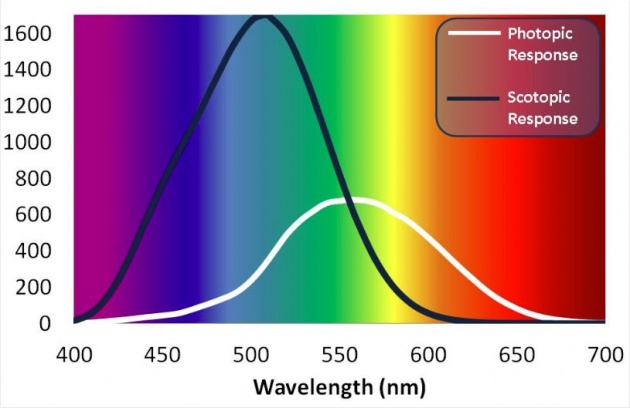
\includegraphics[width=0.8\textwidth]{fig/scoptic.jpg}
    \caption[Color spectrum]{Scoptic and photopic color spectrum. Downloaded from: \url{https://chdv1991.wordpress.com/2011/08/02/the-use-of-red-light-for-illumination/}}
    \label{fig:spectrum}
\end{figure}
Another effect that needs to be mind is change blindness; it refers to the illusion that we as humans perceive our world as if we see everything with high acuity even outside of the fovea. In fact, changes that occur outside our fovea, that do not attract our attention (by motion), are usually missed. A study by \citet{Goddard2013AScale} identified a new type of change blindness to isoluminant color changes. Scoptic vision (low light) and photopic (bright light) vision also differ in color perception; because the rods, which are more sensitive, take over the vision during night, everything appears less saturated and bluer (see \emph{\fullref{fig:flow}}).

Other color models than RGB can be advantageous for color manipulation. The RGB color model is commonly used as it is based on the additive color perception of the human color vision. RGB was already used for analog color photography and is also used in digital photo sensors and RGB displays. Hue-Saturation-Value and Hue-Saturation-Lightness are often used in color pickers as they allow to mix the lightness, saturation, and color hue independently; they match more closely how human vision perceives color-making attributes\footnote{\url{https://en.wikipedia.org/wiki/Comparison_of_color_models_in_computer_graphics}}. Lab color is specifically designed to approximate human vision and implements the  opponent process color theory\footnote{\url{https://en.wikipedia.org/wiki/Opponent_process}}\fnsep\footnote{\url{https://blog.asmartbear.com/color-wheels.html}}. Its L component more closely matches human perception of lightness than the more simple color models\footnote{\url{https://en.wikipedia.org/wiki/CIELAB_color_space\#CIELAB}}. The Fastled LED library makes use of HSV colors with a 'rainbow' hue that has wider yellow band compared to 'spectrum' hues\footnote{\url{https://github.com/FastLED/FastLED/wiki/FastLED-HSV-Colors}}\fnsep\footnote{\url{https://en.wikipedia.org/wiki/Rainbow\#Number_of_colours_in_spectrum_or_rainbow}}.  

\begin{figure}
    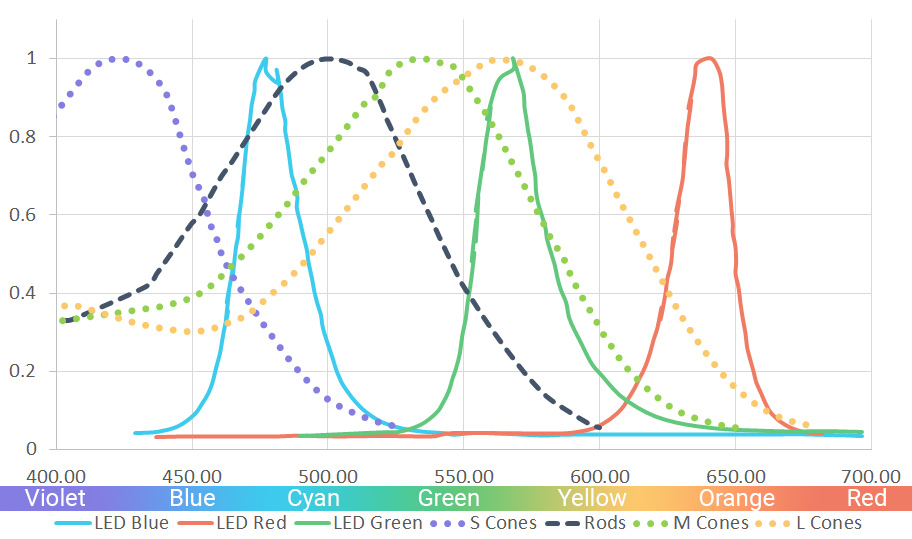
\includegraphics[width=1\textwidth]{fig/spectrum.jpg}
    \caption[LED and Human Spectrum]{Relative Color LED spectrum and relative human spectral sensitivities (nanometer). Graphic by author, Data by \citep{Stockman2000TheGenotype} and extracted from \url{https://en.wikipedia.org/wiki/File:RGB_LED_Spectrum.svg}.}
    \label{fig:spectrumLED}
\end{figure}

In general it needs to be taken care that the stimulus is strong in color, lightness and motion. As red-green color sensitivity declines more towards the periphery, pure red and green color should not be used for important messages. Instead pink\footnote{\url{http://aschoonerofscience.com/science-communication/the-physics-of-pink-why-it-isnt-in-the-rainbow/}} could be used as it stimulates short-wavelength cones and rods more; and so do turquoise and cyan.This might be particularly important as the individual LED light colors usually have a very narrow-spectrum band (see \fullref{fig:spectrumLED}. Even though color perception in the periphery is reduced, the light will get partially reflected and refracted inside the vehicle's cabin and onto the media which is in focus of the users' fovea.  

\section{LED considerations}
\label{sec:LEDconsiderations}
The automotive industry is very concerned about revenue per item. Especially suppliers must take care that they are competitive. LED strips are widely available from Chinese suppliers for very competitive prices. The most popular addressable LEDs are those with the integrated WS2812B microcontroller\footnote{\url{http://www.world-semi.com/Certifications/WS2812B.html}}. Each of the pixels has one red, green and blue LED that can all be controlled from a single data cable. The american 'do-it-yourself' manufacturer Adafruit sells them as Neopixel, and provides good documentation about their possibilities and restrictions \footnote{\url{https://learn.adafruit.com/adafruit-neopixel-uberguide}}. LEDs with the microprocessor SK6812\footnote{\url{http://www.szledcolor.com/productshow.asp?id=930}} often have an additional white LED. This fourth color is necessary for natural white light, as red, green and blue from LEDs usually do not mix a pleasant white. Adafruit sells these LEDs as Neopixels too; this is a bit misleading because they use a slightly different protocol as they have another 8-bit channel in the data signal for the white component of each pixel. As the light bar is planned not just to deliver light signals but also work as a reading light and room lightning, a white component is necessary for more pleasant light. There are also addressable LEDs with the APA102 available that run a lot faster (20Khz vs 600 Hz) but are also less economic. Adafruit brands them as DotStar. 

The LEDstrips are widely available with densities of 30, 60 and 144 Pixels per meter.
With the amount of pixels there are a few trade offs to be considered. More pixels means that each pixel is closer to the next one. This will result in smoother color distribution and higher brightness of the LEDs. But it will also result in a higher current draw, higher price, more use of RAM and processing power and most importantly slower refresh rate. An Arduino Uno\footnote{\url{https://en.wikipedia.org/wiki/Arduino_Uno}} is not capable to control 4m of 144 pixel/m strips due to its Ram constrictions. Each pixel requires 4 bytes of RAM,  thus a 144 LED strip will require 576 bytes of RAM per meter; the Arduino Uno does only have about 1kB Ram available if Libraries are used. Therefore, the strips with 60 pixel/m, which fit exactly in the Ram requirements, with a chain of 60LEDs * 4m * 4 byte = 960 byte, were used.

\begin{figure}
    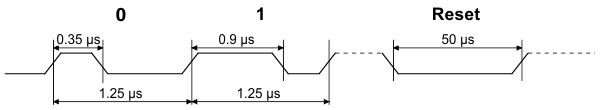
\includegraphics[width=0.8\textwidth]{fig/pololu}
    \caption[LED Specification]{Timing requirements for data transmission to the SK6812 LEDs}
    \label{fig:LEDspec}
\end{figure}

The LED strips WS2812B and SK6812 are controlled with a single data wire, therefore they require precise timing of the data signal for bit banging\footnote{\url{https://en.wikipedia.org/wiki/Bit_banging}}. Arduinos are suited to generate the required signal on their Data Pins. Moreover Arduinos are well supported by some open source libraries. Frequently used are Adafruit Neopixel and Fastled\footnote{\url{http://fastled.io/}}. 

Depending on the amount of pixels one LED strip can draw considerable amounts of current. For the chosen RGBW LEDs of 4m length with a total of 240 pixel the max current they might draw can be calculated as 240 * 80mA / 1000 = 19,2 Amps. However, if the LEDs are programmed appropriately it can be made sure that they do not draw this much power. It should be taken care that red, green, blue, and white are not turned on per pixel and across the whole strip at once. If we plan to use these pixels with just 40mA the estimate current draw is 240 * 40mA /1000 = 9,6 Amps. The pixels and data line use 5 volts. Power supplies with 5V and 10 Amps are more widely available and it is also possible to get these 10 Amps * 5 V = 50 watts from a car battery. 

\section{Software Prototype}
\label{section:software}
The software to control the light strips needs the following minimal software components:
Software bit banging for communication with the light strips, pixel mapping for spatially correct presentation, frame selection to merge all current animations by importance, individual animation looping and an event trigger. 

\begin{figure}
    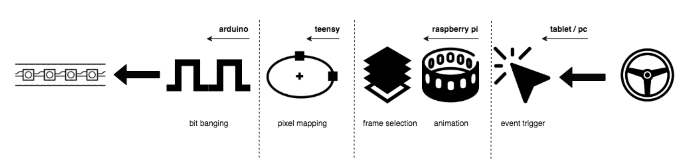
\includegraphics[width=1\textwidth]{fig/softwareflow-}\hfill\
    \caption[Software Flow]{Flow from higher level (right) to lower level software (left)}
    \label{fig:flow}
\end{figure}

In \emph{\fullref{fig:flow}} three possible options for separating the lower levels from the higher level software are depicted. This distinction needs to be made because higher level processing devices such as PCs, tablets and Raspberry Pi do not have the right hardware interface to communicate with the LED strips; while the microprocessors such as the Arduino and teensy do lack the processing power and graphical interface to realize the application. 
The communication between front and back end is ideally wireless and to reduce complexity ideally only one microprocessor and one controller (tablet / pc) should be used.  

\subsection{Arduino Prototyping}
\label{arduino}
The first prototype was done with the bare LED strip and an Arduino. To protect the LED strip from damage a few resistors and capacitors need to be wired up\footnote{\url{https://learn.adafruit.com/adafruit-neopixel-uberguide/powering-neopixels}}. The LEDs proved to be bright enough for peripheral vision during daylight inside of a car at that point of time. There are a few downsides with prototyping directly on the Arduino: Every change of code needs to be compiled on the PC and uploaded from there to the Arduino. Arduinos have to be programmed in Arduino Style C, floating point calculations can take long and smoother animations require to be abstracted in mathematical functions. Moreover, it is a common practice to save  animations in prepopulated arrays to speed things up. This is not an option for this prototype as animations should be mixed together in real time depending on external inputs. Finally, the shape of the LED strips should be taken into account, e.g. animations should not just run from one end of the strip to the other; it should be possible to remap the animations to differently shaped LED strip configurations. 

\subsection{Processing}
\label{ssec:processing}
\begin{figure}
    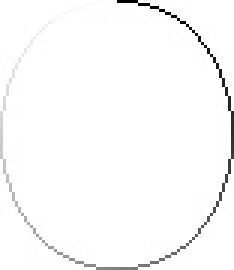
\includegraphics[width=0.25\textwidth]{fig/240id}
    \caption[Pixel Mapping]{Pixel mapping for a LED chain of 240 LEDs to the shape of an ellipse}
    \label{fig:Pixel}
\end{figure}
Instead of rendering the animations on the microprocessor itself, they can be rendered on a PC and forwarded to a microprocessor over the USB port or other channels. 
A small application for prototyping with the processing framework was written. This application allows to visualize the animations on screen and send the animations to the Arduino for display on the LED strip. To map the positions of the 2D animation plane to the LED's identification number from 0-239 a lookup table was used. The lookup table was created with a modified Bresenham algorithm \citep{Raheja2006MidpointAlgorithm}: It draws an ellipse clockwise and increase the ID number with each pixel. In \emph{\fullref{fig:Pixel}} the 78x90 window and the ellipse that corresponds to the physical configuration of the strip are depicted. The resolution of the lookup table depends on the number of LED pixel. Once the lookup table is created it can be stored in some file format i.e. as an image and be reused for each rendered frame. This allows to easily reconfigure the mapping and physical configuration of the light strip. 

The animations should all be very smooth without stutter and visible edges. Therefore, all animations should have a smooth fade to it. When drawing to an animated plane these effects can be easily achieved with gradients and color fades. In processing you can therefore easily draw spherical and rectangular gradients of different sizes colours and transparencies to create animations. Each of the rendered frames of  mapped color data is sent with a simple protocol  facilitating start and end markers over the serial port to the Arduino. Each color is an 8-bit integer. To make space for start and end markers the highest brightness values were omitted. Thus, the actively used width per channel are 0-253 and each frame has a payload of 962 bytes. 


\begin{figure}
    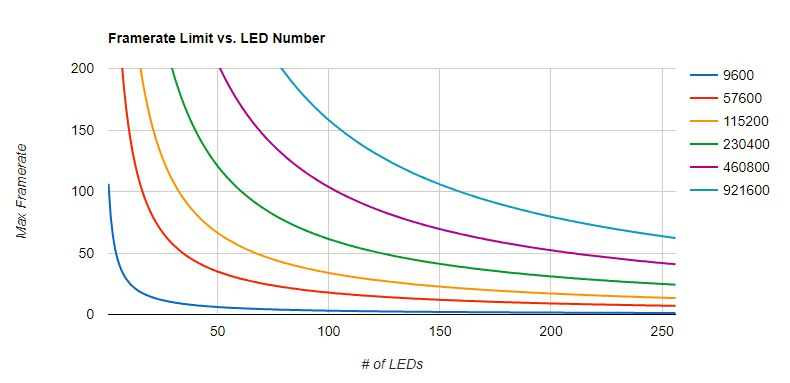
\includegraphics[width=\textwidth]{fig/FPS.JPG}
    \caption[Framerate Limit of RGB LEDs]{Framerate Limit for RGB LED chains with different baudrates. Image adapted from: \url{http://www.partsnotincluded.com/ambilight/calculating-adalight-framerate-limits/}}
    \label{fig:FPS}
\end{figure}

The animations can be drawn and layered with this application, which enables to test  animation speeds, shapes and colors. Moreover, it allowed me to easily show these animations to colleagues and refine them so that they can intuitively be understood. One identified shortcoming is the animation speed. Even though the application achieved continuously more than 40 frames per second on the LED strip some fast animations do not feel as smooth as they could be. The provisional conclusion is that, because of the large distance between the pixels, the frame rates of an LED strip should be even higher than the recommended minimal frame rates for displays. Also, the serial port communication with the Arduino in combination with the bit banging for communication with LEDs seems to be a bottleneck; the single threaded Arduino interrupts once a message is received via the serial port and vice versa while the pixel colors are transmitted to the LED strip the serial port is blocked. This Ambient display has to deliver quick information in a smoothly animated manner; the framerate limitation of the LED chains becomes a severe issue\footnote{\url{http://www.partsnotincluded.com/ambilight/improving-adalight-framerate/}}. 

\subsection{Bluetooth}
\label{ssec:bluettoth}
It is not feasible to use a whole Java Processing application on a desktop computer to control the system inside a car; it will be clumsy to control the light signals from a computer and also difficult to integrate it, if so, with the CAN bus of a car. The lowcost Beetle BLE\footnote{\url{https://www.dfrobot.com/wiki/index.php/Bluno_Beetle_SKU:DFR0339}} was used to test if it is feasible to create a wireless system with an Arduino microprocessor. The Beetle Ble has a smaller prototyping board than the Arduino and supports Bluetooth UART communication. This makes it possible to communicate to the Arduino also with a tablet or smartphone device. The processing application was ported to use the Bluetooth serial port instead of the usb serial port. The payload for 40 fps is 38,48 Kbyte/s.
Each frame was still rendered by the Java Processing application and then send to the Arduino, which just further forwarded the data to the LED strip. Unfortunately, this approach led to jittered frames as the Bluetooth data was not received in order by the Arduino sketch. Multiple approaches did not lead to satisfactory solutions. The implementation of handshaking (see \emph{\fullref{ch:glossary}} significantly. Using another 16 bytes in the payload to signal frame order lead to splitted frame messages; the first half of the message did not always arrive synchronous with the second half. The approach producing the smoothest transitions was to send messages at a very low frame rate of 10 fps and interpolate all pixel values in between. Even though the transitions were smooth they did not render exactly as intended. Small and fast moving parts, for instance, do not appear to move quickly across the strip but to light up individual pixels instead. 

\subsection{Smooth animations}
\label{ssec:smooth}
Addressable RGB-W LEDs are more difficult to work with. They are less common and thus, there is less documentation and libraries available. A better choice would have been to use faster LEDs without the white component such as APA102. Even for the slower RGB LEDs without the white component dedicated hardware exists that allows faster and smoother animations. For example, the Fadecandy\footnote{\url{https://github.com/scanlime/fadecandy}} and OctoWS2811\footnote{\url{https://github.com/PaulStoffregen/OctoWS2811}} LED libraries use a Teensy microprocessor instead of an Arduino; this allows to handle far more LEDs with high frame rate as the communication with multiple LED strips can happen parallely and not serially. Unfortunately, these libraries and hardware configurations usually only support the WS2812 (RGB) Type of LED strips. DMX via Ethernet is the state of the art protocol for concert light shows. Even with this protocol strips are restricted by the refresh rate of LED strips, speed of data transmission, amount of total pixels and amount of pixels in one chain\footnote{\url{https://support.troikatronix.com/support/solutions/articles/13000042899-controlling-led-strips-via-artnet}}\fnsep\footnote{\url{http://help.madrix.com/tutorials/html/index.html?hidd_dmx_addresses.html}}.  

\subsection{Raspberry Pi}
\label{ssec:raspberry}
To increase the refresh rate up to acceptable smoothness the platform had to be switched. I chose to recode the application to run on a Raspberry Pi with the incentive to make use of its multithreading capabilities. To do the calculation and mapping of animations as well as the bit banging on the same device. Besides, to run the software and hardware on an embedded system delivers the proof that it can be integrated cheaply into a vehicle. This way the only external input to the microprocessor, which is in control of the bit banging, is the event input. Events are only triggered every few seconds instead of milliseconds. Then, the bottleneck of Bluetooth or serial port communication speed is effectively eliminated. 

\subsection{Pulse Width Modulation}
\label{ssec:pwm}
%more to this maybe
Multithreading capabilities of the CPU can be an advantage because multiple processes can run in parallel, however, it is a disadvantage, too, in that it is not straightforward to control the sk6812 LEDs from the Raspberry Pi platform. The standard GPIO ports are not capable to do the bit banging with the timing that is required by the single wire LED strips. This is the reason why the common LED strip libraries do not support the Raspberry Pi. However, there exists one solution to still get the single wire LED strip to work on a Raspberry Pi, which is to make use of the pulse width modulation channel of the Raspberry Pi's Broadcom chip. This channel is usually used to create the analogue audio signals for the playback of music. Because the audio playback is stereo, two pulse width modulation channels exist. Thus, it is possible to drive two chains of LEDs independently in parallel, which almost doubles the maximal framerates. The only library that is publicly available so far is by Github user \cite{Jgarff2018UserspaceLEDs} and fortunately even provides a Python wrapper to control the pixel. This is advantageous because then the whole software can be written in one programming language. 


\subsection{CAN Bus}
\label{ssec:CANbus}
The CAN bus is short for Controller Area Network bus developed by Robert Bosch \footnote{\url{https://www.can-cia.org/can-knowledge/can/can-history/}}. It is a communication standard designed to allow microcontrollers and devices to communicate with each other inside the car without a central computer or huge amount of cables. A lot of car data and sensors are send through this bus system. 

Interesting for the development of this application are mostly the steering wheel angle, current speed, acceleration, braking force and blinker position. With access to these signals some of the light signals could be automatically triggered and some others could be customized to the current driving conditions. For example the steering wheel angle could be used to tilt the start direction of animations or the blinker could be used to identify when a lane change is about to happen. Unfortunately, the Robert Bosch CM department has not the appropriate license to retrieve all data from the CAN Bus of the Nissan Cube. Robert Bosch works on Clusters and Infotainment for Nissan, thus, only the information necessary for these products is available. Unfortunately, steering wheel, braking and acceleration are not available. 

The CAN bus is usually not encrypted though, this means that in theory all data is available for a hacker with access to the ports of the car \footnote{\url{https://motherboard.vice.com/en_us/article/ae33jk/we-drove-a-car-while-it-was-being-hacked}}. The difficult part is however to reverse engineer all these messages. Thousands of CAN signals are sent through the network. Thus, it is a very time consuming process to find out what the actual bits of signals are depicting.  Almost all software to tap into CAN data is proprietary software from the car industry. The most notable exception is the Panda by Comma.ai ( \emph{\fullref{sec:Data}}), which is a dongle that plugs into the OBD port of vehicles and streams CAN data to phones or computers. With this dongle and the open source software cabana the CAN data from the Nissan Cube was analyzed. The software is capable and helps to reverse engineer CAN Data for hacking vehicles or retrofitting them with self-driving features. The current speed could be extracted from a captured test drive with the Nissan Cube. However, open doors, braking and steering wheel angle were not identified. Thus, it was decided to not further spend time on this effort before other more significant components got realized. 

\section {Software components}

\begin{figure}
\centering
    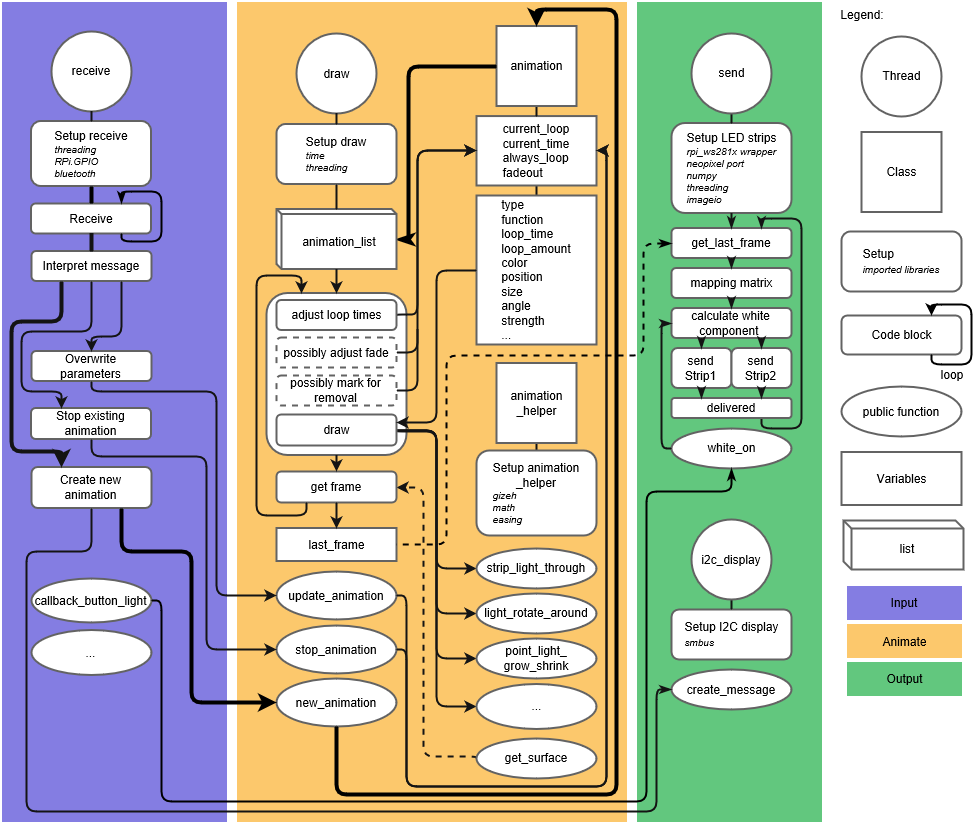
\includegraphics[width=1.1\textwidth]{fig/Flow.png}
    \caption[Software Diagram]{Individual Components of the Application}
    \label{fig:software}
\end{figure}
% This introduction maybe somewhere else
The application is written in Python on the Raspberry Pi. Python was chosen because it is the best environment to create all the interfaces between the individual components. Most importantly the rpi\_ws81x library comes with a Python Swig wrapper\footnote{\url{https://en.wikipedia.org/wiki/SWIG}}. In production a lower level programming language would be preferable. The application depends on threading because receiving Bluetooth messages, sending the data to the light strip, showing messages on the LCD display and rendering the animations should happen independently. If a message arrives the LED strip should not stutter and computationally more heavy animations should play frame rate independently. 
In \emph{\fullref{fig:software}} a software overview is shown: In purple are the parts that deal with input, in yellow the parts that deal with animation and in green the parts that deal with the output. The three major time consuming loops are ‘receive’ in the receive thread, ‘draw’ in the draw thread and ‘send Strip1’ together with ‘send Strip2’ in send. The bold line shows the path of an incoming event that gets saved as an animation in the 'animation\_list'. The dotted lines show how the send thread receives the latest animation frame and how the draw class receives an animation frame (surface) from the 'animation\_helper'. 
Receive is the master thread, it set ups the Bluetooth channel and waits for connection of a device. Once it receives a message it interprets the input and calls the appropriate functions in the draw class. Furthermore, within 'receive' callback functions for the four arcade buttons are initialized. 
'I2C\_display' uses the SMBUS to communicate with a demultiplexer\footnote{\url{http://shallowsky.com/blog/hardware/multiplexing-io-expanders.html}}, which controls the 8-bit liquid crystal display. The demultiplexer is necessary as otherwise too many GPIO ports from the Raspberry Pi get blocked. 

The send thread is used for communication with the LED strips. It uses the rpi\_ws18x wrapper for direct memory access for pulse width modulation with the Broadcom microprocessor on the Pi. First in the send loop the last animation frame is retrieved from the animation class, then the mapping matrix is applied to filter the animation frame. The mapping matrix is stored in a black \& white image. This way the mapping matrix that was created for the processing application can be reused. Furthermore, very specific LED strip shapes could be drawn in graphic applications by hand. For each of the 240 remaining pixels the white component is calculated. The animations are RGB only and the White pixel depends on the reading light button status. As the animations should be clearly visible even when the reading light is on the white component it is inverse logarithmic dimmed depending on the RGB values. The NumPy library\footnote{\url{http://www.numpy.org/}}is used to speed up matrix operations. The pixel color values are then reorganized as the animation image is RGB but the LED strip is GRBW. The bit patterns are precast in Ram and then transmitted as one entity. 

The draw class takes care of all animations during their lifetime. The public function new\_animation is used to create an instance of animation. All animations are created depending on their type and stored in a list. Each animation has preset values (as defined in Section \emph{\fullref{sec:Lightdesign}}) such as color, position or loop\_time and values that change during execution such as current\_time. For each drawing iteration each animation's loop times in the animation list get updated. The actual drawing is done by the animation\_helper. It uses Gizeh\footnote{\url{https://github.com/Zulko/Gizeh}}, a vector animation library, math and easing functions for drawing. Multiple options for animations are available via the animation helper. It takes care that consistent looping animations are created but allows to adjust certain variables such as thickness, color or angle. The animations use transparency so that multiple animations can get overlayed. A possible extension might be to use different blend modes than simple overlays. The light messages are drawn by order of creation, which means that new animations overlay older animations. Once each animation in the list is drawn the full frame is retrieved. Then after a short delay the draw loop starts again. Some animations are stopped manually otherwise they loop forever. When they are stopped and started they get faded in and out. Only after their life time, are they removed from the animation list. 
\section{Demonstrator}

\begin{figure}
     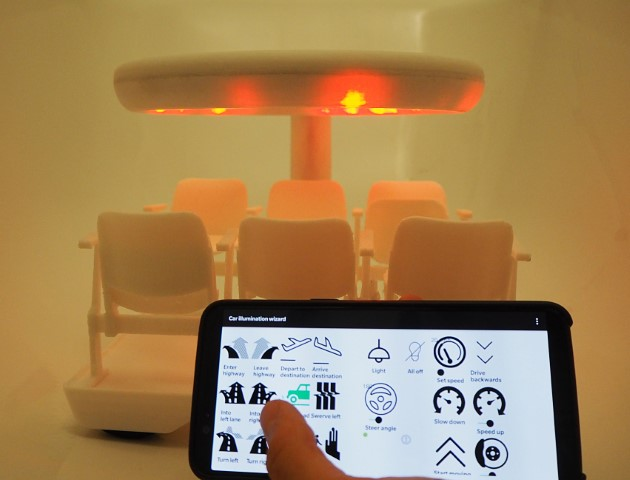
\includegraphics[width=\textwidth]{fig/public.JPG}\hfill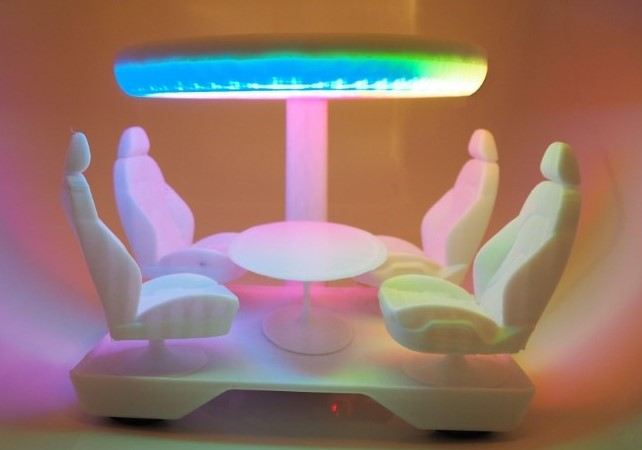
\includegraphics[width=\textwidth]{fig/private.JPG}
    \caption[Desktop Demonstrator]{The miniature demonstrator and control of it (Left:  Public vehicle configuration. Right: Private configuration.)}
    \label{fig:demonstrator}
\end{figure}
\begin{figure}
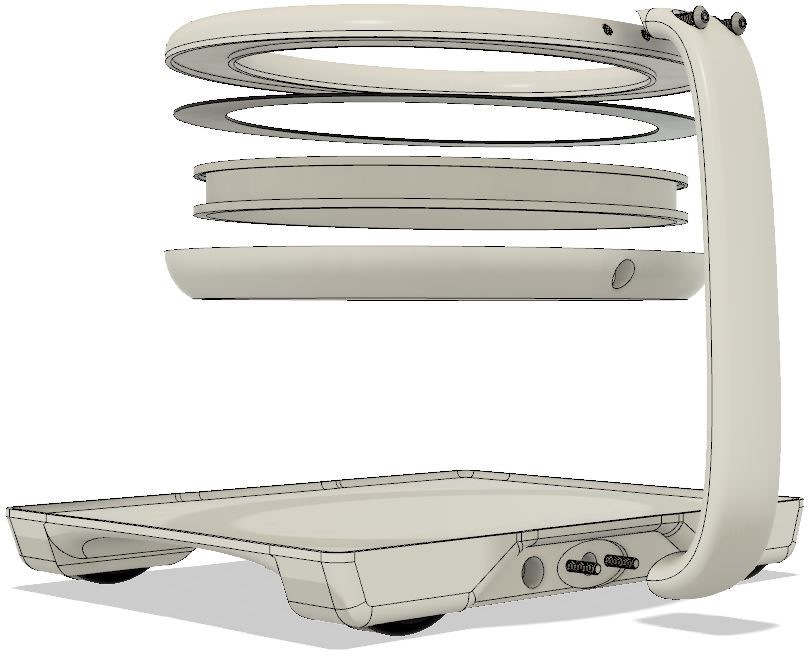
\includegraphics[width=0.9\textwidth]{fig/explosion.JPG}
    \caption[Explosion-view Demonstrator]{Explosion view of the light diffusor}
    \label{fig:demonstratorExplosion}
\end{figure}
During the development of the Light Interface, I spent a lot of time in the test vehicle: for debugging, to fine tune the animations, to add additional functionality and to teach the interaction wizard (See: \emph{\fullref{sec:study}}) how to use the wizard interface. It is very cumbersome to develop software inside a vehicle because of its inconvenient ergonomics and limited access to infrastructure (power, internet, and heating), this is the first reason why I created the miniature demonstrator ( \emph{\fullref{fig:demonstrator}}). It can be used as a desktop development tool. Furthermore, it is useful to have something haptic to show during workshops, exhibitions or to interested partners. Finally, the demonstrator allows car interior designers to test how different interior configurations work in collaboration with the light interface. The shape only slightly suggests a vehicle and the open platform provides free positioning of varying seat types, seating arrangements and interior fittings on top of it. The furnishing can get rapidly 3D printed or modeled with traditional methods. The electronics are positioned below it and can be controlled with the Bluetooth Android App ( \emph{\fullref{sec:wizard}}) or directly plugged into a computer. The 3D printed demonstrator was modeled in Autodesk Fusion 360. The cables are passing through the neck, which is attached with screws. The light ring consists of 4 parts which are welded together with a 3D pen, and allow the light from two light strips to be redirected downwards through a 3D printed diffusing grid infill. 


\section{Wizard Interface}
\label{sec:wizard}
The light signals need to be controlled by a wizard, hence an application or hardware is required to do so. An app was realized within the Android operating system. It was created for a small tablet so that it can be controlled easily with two hands. Each event can be triggered by its own button. Depending on the type of events these can be triggered once or turned on and off. Furthermore, sliders are used to control interval data. Each event button makes use of a descriptive icon, color feedback and text, to help the wizard quickly trigger events. All icons are creative commons and downloaded from \emph{The Noun Project}\footnote{\url{https://thenounproject.com/}}. For transmission of the events a message protocol was created (See Code: \emph{\fullref{lst:eventmessage}}). These messages are transmitted to the control unit via Bluetooth. 

\begin{lstlisting}[caption={Examples of event messages.},label={lst:eventmessage},language=Python]
<start_moving,loop=1,angle=180>
<brake_now,loop=1,strength=50>
<move_backwards,loop=INF,angle=180>
<move_backwards,loop=OFF>
<highway_enter,loop=3.0>
\end{lstlisting}

The loop can be transmitted as amount of full animation loops \emph{(integer)}, time to play the animation loops \emph{(float)} or as infinite loop duration \emph{(INF, OFF)}. Additional parameters such as angle and strength are send along the event. The wizard can specify them by using the sliders next to event buttons.   
After the first training rounds with the driving wizard and control wizard the buttons in the interface were rearranged according to his preference with the most frequent events close to the left and right border of the screen for quicker usage by two hands in vertical mode (See  \emph{\fullref{lst:eventmessage}}). 

\begin{figure}
    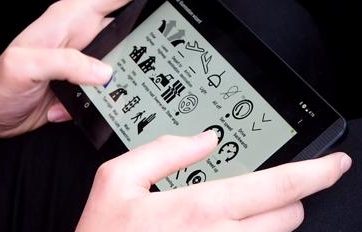
\includegraphics[width=\textwidth]{fig/WizardHands}\hfill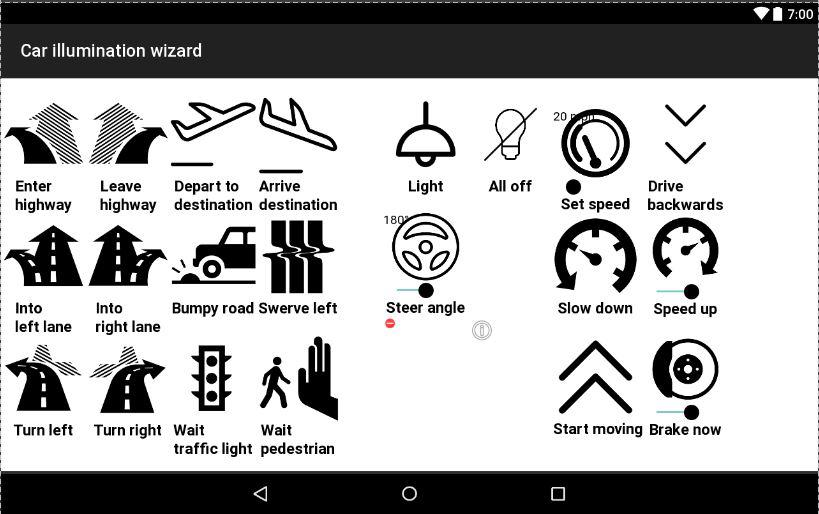
\includegraphics[width=\textwidth]{fig/IlluminationWizard-.JPG}
    \caption[Wizard Tab]{Left: Wizard Tablet. 
   Right: Wizard Interface.}
    \label{fig:wizard}
\end{figure}

\section{Call a Cab App}
\label{sec:capp}
The test subjects should get an idea about what a ride in a potential autonomous cab might look like. For this reason a web app was developed. This app shows the route that will be driven and the participants current location on it. Furthermore, the app is used to call the cab to the studies pick up location. This enhances the impression of an autonomous vehicle and disengages the study subjects further from other human contact. The user presses the 'call a cab' button once he is ready to start the test drive and the wizards receive a push notification on their smartphone through the Pushbullet service\footnote{\url{https://docs.pushbullet.com/}}. This wizards drive the test vehicle to the pick up location and honk to inform the user of the cab's arrival. 

\begin{figure}
    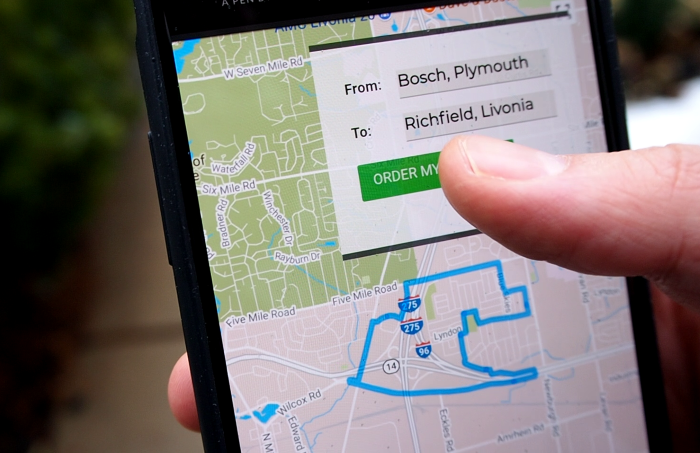
\includegraphics[width=\textwidth]{fig/capp}
    \caption[Call a Cab App]{The web app to call the cab}
    \label{fig:capp}
\end{figure}

\section{Physical components}
\label{sec:physical}

\begin{figure}
    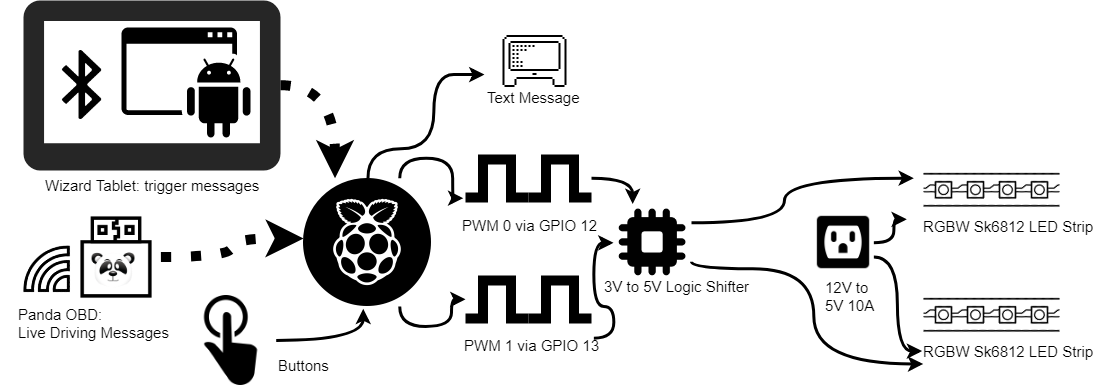
\includegraphics[width=1\textwidth]{fig/wizardfinal}
    \caption[Communication Overview]{Communication between individual components}
    \label{fig:communication}
\end{figure}

\emph{\fullref{fig:communication}} shows the hardware connections of the final prototype. The central hub that all devices communicate with is the Raspberry Pi. It uses pulse width modulation to bit bang the colours to the LED strip. The LED strip is split in half so that each channel controls 120 LED RGBW pixels. The output voltage of the Raspberry Pi GPIO is 3.3 volts. A Logic shifter is used to shift the high voltage bits to 5 volts. The LED strips are powered from the car battery with a step-down regulator (12 volts regulated to 5 volts and 12 amps). The users of the system have access to an emergency stop button, 'Start Ride' button, a 'Guide' on/off button, and a reading light on/off button, which are connected to the Raspberry Pi with a pull-down resistor in place. The driving events are communicated through an Android tab that sends events with Bluetooth to the Raspberry Pi. This allows to easily configure buttons, sliders icons and knobs. The current speed is retrieved via WIFI from the Panda OBD dongle ( \emph{\fullref{ssec:CANbus}}). A small text display is connected with a port expander to the Raspberry Pi (Sub \emph{\fullref{ssec:display}}). 

\subsection{Light bar}
\label{ssec:lightbar}
\begin{figure}
  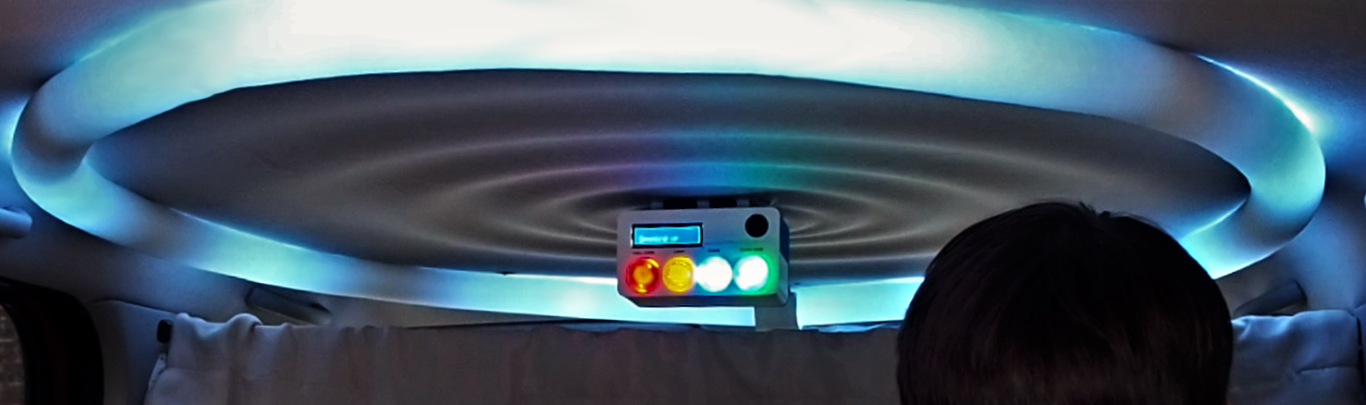
\includegraphics[width=\textwidth]{fig/teaser.png}
  \caption{The ambient display prototype inside the test vehicle (speed up).}
  \label{fig:ambientdisplay}
\end{figure}
The light bar was enclosed by a matte silicon tube. As it does not diffuse the light enough to obscure individual LED pixels a construction out of semitransparent acrylics was designed ( \emph{\fullref{fig:lasercut}}). The design files for the laser cutter use 6 sheets of plywood and 6 sheets of diffusing acrylics. The universal snap fit\footnote{\url{https://tltl.stanford.edu/project/universal-snap-fit}} holds the individual sheets together and connects the upper layer wood with the lower layer of acrylics.  Bosch does not have a laser cutter in the Michigan area. Test cuts with a water-jet did not give high-quality edges to justify the cost. A few price estimates from laser cutting companies in the Michigan area were also out of the justifiable price range. 
\begin{figure}
    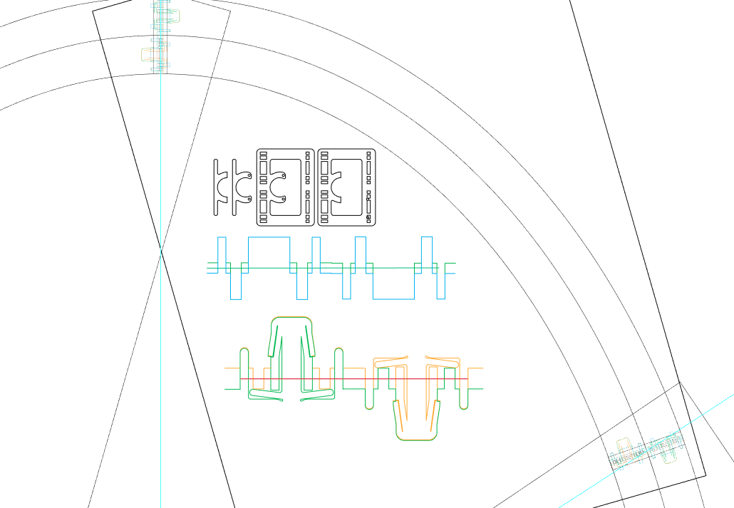
\includegraphics[width=0.8\textwidth]{fig/lasercut.png}
    \caption[Paths for Laser Cutting]{Paths for laser cutting an large ellipse out of diffusing acrylics and plywood sheets (18in x 24in). In the center tube attachments (black), acrylic slots (blue,  enlarged) and interlocking wood mechanism (green and yellow, enlarged) are shown.}
    \label{fig:lasercut}
\end{figure}
Therefore, low cost alternatives were considered. Insulation foam that is used for pipe insulation diffused the light quite well. This material is also used by cheap LED glow sticks. The two parts of the tube were sewn into the ceiling in the ellipse shape and covered by long sections of the insulation foam. 
In the front the tube is hold together, covers connectors and a few electronic parts by a 3D printed housing ( \emph{\fullref{fig:boxes}}). 

\subsection{Control Unit}
\label{ssec:controlunit}
The Raspberry is installed in a housing on the ceiling. It was modeled in a CAD application and then 3D printed. It has cutouts for four arcade buttons that can light up, for a liquid crystal display and for a video camera. The layout and placement are inspired by the Waymo self driving vehicles (Fig:\emph{\fullref{fig:fig-waymo}}). There is a button for starting the ride and for emergency stops (pull over); this might give the passenger a sense of control. Furthermore, the Waymo vehicle has a 'lock doors button' and a 'call for help' button. These two were omitted in the favor of a 'reading light' button and a 'Guide on/off' button. Further, a wide-angle camera is housed in the control unit. It has a comparatively good low light quality and can be operated over WiFi. It is used to record the test drives without making participants feel like they are being completely monitored and is needed for a fully autonomous vehicle to film passengers, too. 

\begin{figure}
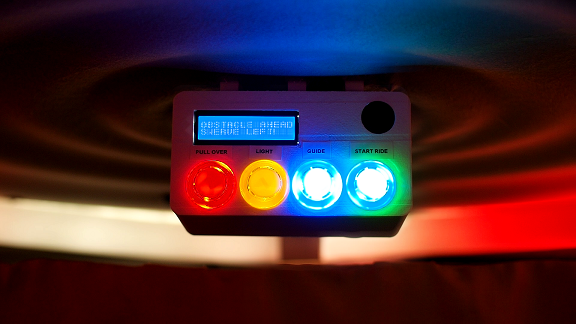
\includegraphics[width=\textwidth]{fig/monitor.png}\hfill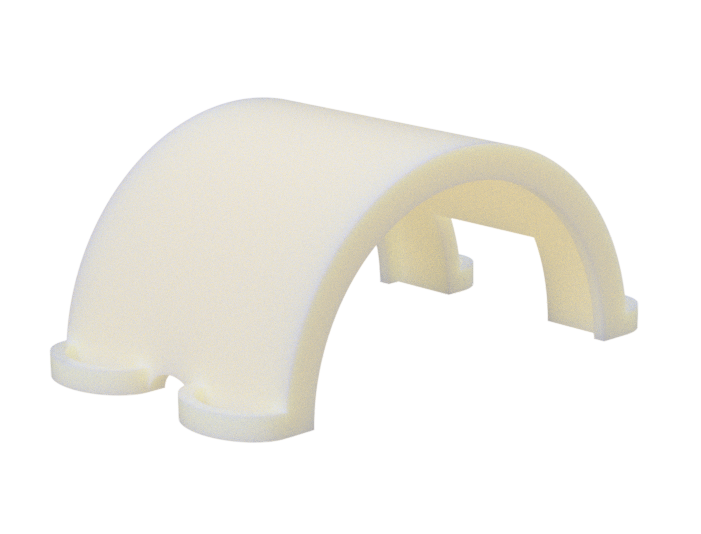
\includegraphics[height=0.36\textwidth]{fig/KabelH.png}\hfill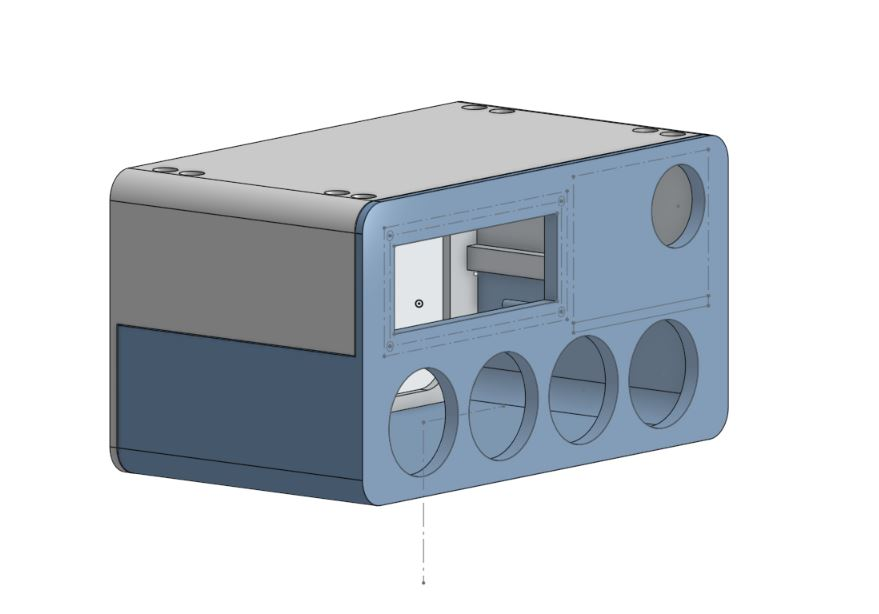
\includegraphics[height=0.36\textwidth]{fig/controlBox2.JPG}
\caption[Control Unit]{Top:Control unit inside the car prototype with lit-up buttons. Bottom: 3D files for foam roll connector and contorl unit.}
\label{fig:boxes}
\end{figure}

\subsubsection{Display}
\label{ssec:display}
As the light display will not be used over enough time by the participants to internalize the different light signals meanings, a small display should help the passengers to learn the meaning of them. An LCD display \emph{(HD44780)\footnote{\url{https://en.wikipedia.org/wiki/Hitachi_HD44780_LCD_controller}}} was integrated into the control unit. It is connected to the Raspberry Pi over the I2C protocol. Since it requires a lot of ports for communication 
a port expander was used\footnote{\url{https://www.robotshop.com/letsmakerobots/drive-a-standard-hd44780-lcd-using-a-pcf8574-and-i2c}}. The text messages on the display were triggered by the light messages. The correspondence between light events and display messages is shown in (\emph{\fullref{tab:display}}).

\begin{table}[ht]
\caption{Correspondence Between Light Events and Display Messages}
\label{tab:display}
\footnotesize
\begin{tabular}{ll}
\toprule
Type        &  Message                      \\
\midrule
turn\_left            & About to turn left           \\
turn\_right           & About to turn right          \\
start\_moving         & Start moving                 \\
move\_backwards       & Driving backwards            \\
lane\_left            & Into: left lane              \\
lane\_right           & Into: right lane             \\
depart\_todestination & Have a good ride!            \\
arrive\_destination   & You arrived!                 \\
highway\_enter        & Entering left                \\
highway\_leave        & Exiting right                \\
wait\_trafficlight    & Waiting for: traffic lights  \\
wait\_pedestrian      & Waiting for: pedestrians     \\
uneven\_road          & Uneven road!                 \\
swerve\_left          & Obstacle ahead: Swerve left! \\
brake\_now            & Braking                      \\
slow\_down            & Slowing down                 \\
speed\_up             & Speeding up                  \\
speed\_keep           & Driving                      \\
default               & Autopilot is active         
\end{tabular}
\end{table}




\chapter{Evaluation}
\label{ch:evaluation}
\section{Test drives}
Participants should be tested on the real road as simulators may allow testing for quantitative data such as reaction time but hardly allows to recreated fear or discomfort ( \fullref{sec:studies}. 

\subsection{Study Setup}
\label{sec:study}
In a counterbalanced, 2x2 experimental design setup, 
14 participants first rode either route A or route B, with the feedforward information either turned on or off. Next, they rode in the inverse constellation (\fullref{tab:blocking}). Test rides each had a total length of 45 minutes. 
The researcher welcomed participants in the lobby of the Bosch Technical Center in Plymouth and collected concent. Then subjects were on their own. They received a detailed instruction (\fullref{fig:instruction}) and were positively 'primed'\footnote{\url{https://www.nngroup.com/articles/priming/}} about autonomous vehicles with a scenario.
\begin{figure}
     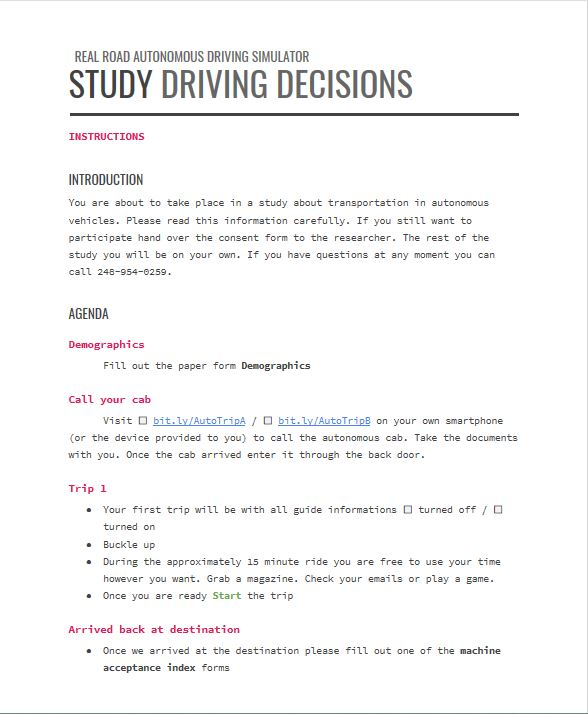
\includegraphics[height=0.31\textwidth]{fig/instru1.JPG}\hfill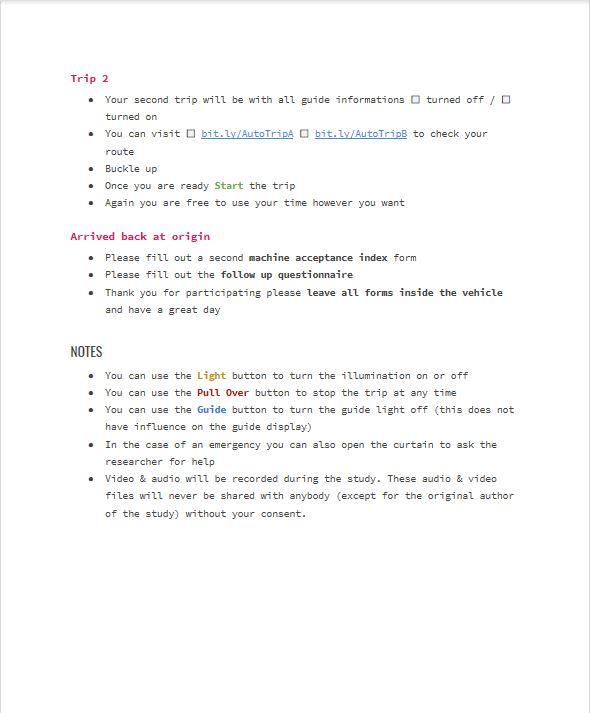
\includegraphics[height=0.31\textwidth]{fig/instru2.JPG}\hfill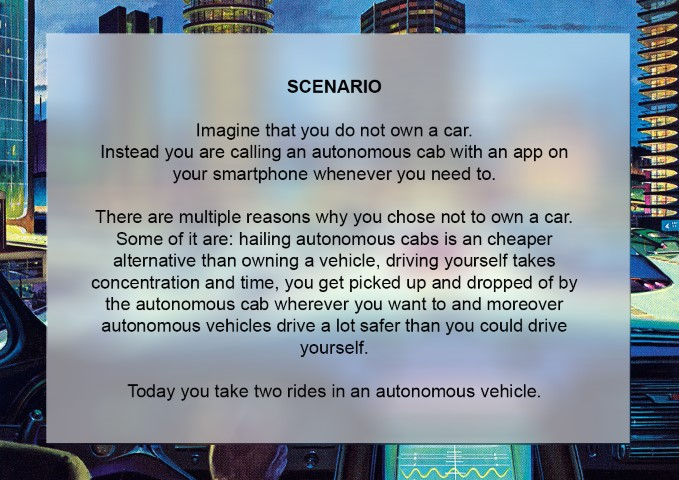
\includegraphics[height=0.31\textwidth]{fig/future-city-scenario_854.jpg}
    \caption[Study Instruction]{Left: Instruction. Right: Scenario. (Full resolution versions are attached in the digital appendix)}
    \label{fig:instruction}
\end{figure}

They called the cab with the web app (\fullref{sec:capp}) as instructed. The cab arrived in front of the lobby and honked to inform of its arrival. Because of the angle at which the vehicle approached and a curtain that separates passengers in the back from the wizards in front, participants could not establish eye contact. Once buckled up they pressed the 'start ride' button. 
\begin{figure}
     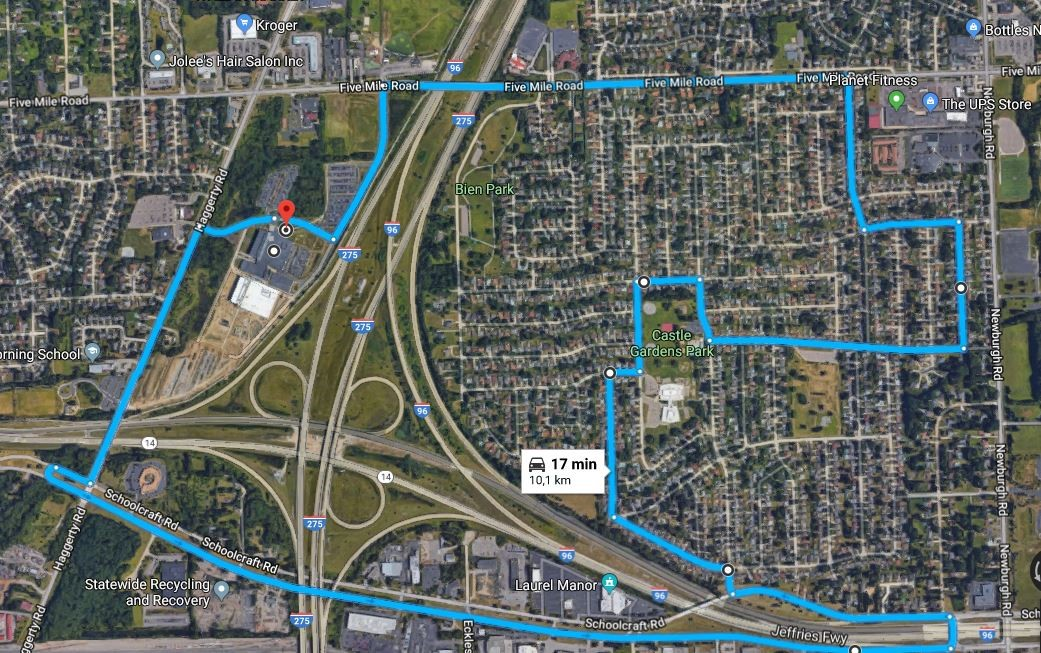
\includegraphics[height=0.31\textwidth]{fig/RouteA_Mittel.JPG}\hfill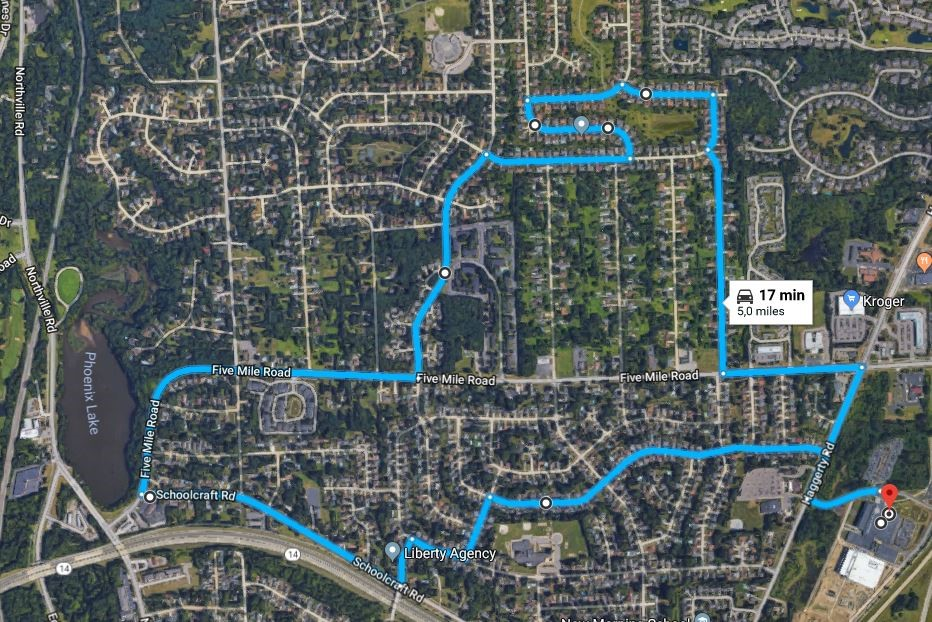
\includegraphics[height=0.31\textwidth]{fig/RouteB_Mittel.JPG}
    \caption[Test routes]{Test routes. Left: Livonia (17min, 7.1km). Right: Northville (17min, 8.0km)}
    \label{fig:routes}
\end{figure}
The routes started and always ended at Bosch Technical Center in Plymouth. The tour through Northville was longer and had a higher top speed as parts of it were on the highway (60mph). Both tours took approximately 17 minutes (\fullref{fig:routes}). The tours differed so that participants did not have to drive the same route twice and did not pay less attention the second time (learning effects). 
During each of the rides, the subjects were videotaped and could use their time freely. The participants filled out one pre-study questionnaire, two of the same trust in automation questionnaires \cite{Jian2010,Koo2015} and a post-study questionnaire. In the feedforward-information-on (guide on) condition the cars decisions were augmented through the interaction wizard.

\begin{table}[]
  \caption{Blocking of study participants}
  \label{tab:blocking}

\begin{tabular}{@{}l|llll@{}}
\toprule
                    & First Livona & First Northville &  &  \\ \midrule
First without guide & 3+2          & 3                &  &  \\
First with guide    & 3            & 3                &  & 
\end{tabular}
\end{table}

\subsection{Vehicle}
For the on the road tests a red Nissan Cube test car (\fullref{fig:testsetup}), which was used earlier for software testing of an infotainment system and was thus available for prototyping, was used. Even though the interior already came of age the outside looks like a cute futuristic cab. The chassis of the vehicle drives a bit jerky. Smoother acceleration and brake might influence the wellbeing of passengers positively; however, the design of the vehicle is different enough from average vehicles to be mistaken for an autonomous cab, and the Cube is spacious in the back. The car was thoroughly cleaned before user testing, and the components were sewn into the ceiling.

\subsection{Separation}
The test subjects should be separated from the researcher. They should neither be able to make eye contact with them nor should they be able to observe the gestures and behavior of the driver and control wizard. Ideally, the test subjects know neither who drives the vehicle nor that somebody controls the vehicle at all. \cite{Baltodano2015} used a vertical separator. Their research was for autonomous driving in level 2 and 3; this research examines vehicles with self-driving capabilities in the highest category. The passengers do not have to take over control; the vehicle drives autonomously at all times. In such vehicles the passengers will not have access to a steering wheel, they might sit backward, lying down or in the back seats. In regular cars view onto the street is already constrained in the back. To be able to see out through the front, back seat passengers have to move their head to the center. Moreover, in a lot of cabs and limousines, the view out through the front is blocked. Therefore the scenario with a horizontal separator (\fullref{fig:testsetup} comes close to reality. 
\begin{figure}
    \includegraphics[height=0.38\textwidth]{fig/test-setup-hori}\hfill\includegraphics[height=0.35\textwidth]{fig/enter.png}
    \caption[Driving Simulator]{Left: Seating of wizards and test subject. Right: Test subject entering the autonomous driving simulator}
    \label{fig:testsetup}
\end{figure}

A blackout curtain was attached to the b pillar to separate the researcher from the passengers. It blocks shadows so that the silhouettes from the researchers are not visible. Light color and texture were used so that even though it is right in front of the passengers, it does not feel close and oppressive. It was attached with a sturdy metal rope and needles so that it stays in place. The curtain was high enough that the heads of the driver and wizard could not be seen and low enough so that most people should be able to glance at the front of the light bar.  The control box was attached slightly above the curtain and cables were laid to the front and through the paneling to the battery. 

\subsection{Video Analysis}
\label{sec:videoAnalysis}

I recorded video of the cabin as increasingly, it is being recognized that capturing behavioral data from participants, such as facial expressions or head movements, may be a more accurate representation of how and what they feel and a better alternative to self-report questionnaires that interrupt participant’s emotions and cognitions during performance \cite{Ahn2011UsingPrediction}.

\begin{figure}
    \includegraphics[width=0.5\textwidth]{fig/PieTotal.png}\includegraphics[width=0.5\textwidth]{fig/PieTotalNo.png}
    \caption[Total Times of Focus of Attention]{Total Times of Focus of Attention. Left: Guide On condition, Right: Guide Off condition}
    \label{fig:totalPie}
\end{figure}

The first impression of the participants when they enter the vehicle was that: five appear a little bit tired (yawning, sleepy eyes), five seem engaged (awake, looking out of the window, rereading the instructions), two skeptical (frown, contemptuous), one is relaxed (closing eyes), and one participant appears to be frightened (holding onto handrails). Participants shifted their attention constantly between inside the vehicle and outside the car; this is very different from drivers who have their eyes always on their road and passengers who are immersed in non-driving tasks. 
Three participants were listening to music or audiobooks on their own devices. Two participants were looking onto their smartphone for more extended periods (but less than 1/4 of the driving time), two participants tried to use their phone initially but stopped after a while, and three participants checked their phones briefly (for periods of a few seconds). One person closed their eyes for roughly 1/3 of the drives. 

We can see in the video how most of the participants used the information that was available to them: People checked the screen regularly and the light bar sparsely; Some people used the web app or opened Google maps to check their location; If they felt, heard or saw something they were checking the windows, the light bar, and the screen. Because I did not track the location of the test car it is difficult to relate the events, messages and peoples reactions with high precision, however, it appears that the typical chain of events was: participants head down - light message triggered - participant looks out of the window - event is executed in reality - participant checks the screen - the participant looks down again. 

No person used the 'Pull Over' button. A few people used the Light button to turn the light on to fill out the forms, and a few people turned the guide light off for a moment but turned it back on after having the function tried out. 

I analyzed half of the rides statistically as the light conditions allowed to see the subjects throughout both tours (n=7). The videos were coded with ELAN\cite{Wittenburg2006ELAN:Research}. Noticeable gestures and speech were written down. I categorized the direction of attention throughout the whole ride into the categories: Close Window, Far Window, Down, Far into Close Window, On Controller, Directly Onto Light Bar, Straight, Back, Eyes Closed (See \fullref{fig:videocode}. These were combined into attention out of the vehicle (Windows), inside the vehicle (Down, Straight, Eyes Closed) and onto the Information (Controller, Light Bar). The individual events were averaged into duration's and normalized and summed into totals.
\begin{figure}
    \includegraphics[width=1\textwidth]{fig/StefSas.JPG}
    \caption[Video Coding]{Video coded test ride}
    \label{fig:videocode}
\end{figure}
Because the data is approximately normally distributed (Shapiro-Wilk) ratio data, I used Paired Samples T-Tests to compare the times with guide on against guide off. In the 'guide on' condition, attention was marginally-significant\footnote{\url{https://www.psychologicalscience.org/publications/observer/obsonline/rise-in-reporting-p-values-as-marginally-significant.html}} longer outside the vehicle and significantly shorter inside the vehicle. These effects were all large \fullref{tab:totalVideo}. People were paying more attention to what was happening outside (\fullref{fig:attentionTotal}); possibly they tried to consciously match what the messages indicated with what happened outside or the light just directed their attention unconsciously back up. Thus one might conclude that the light messages lead to more attentive rides. 

\begin{table}[]
\label{tab:totalVideo}
  \caption{Paired Samples T-Test of total time differences}
\begin{tabular}{@{}llllll@{}}
\toprule
 & statistic &  p & Mean diff. & SE diff. & Cohen's d \\ \midrule
Outside & 2.206 &  0.070 & 2.139 & 0.970 & 0.834 \\
Inside & -2.532 &  0.045 & -2.218 & 0.876 & -0.957 \\
Information & -0.050 &  0.962 & -0.028 & 0.572 & -0.019 \\ \bottomrule
\end{tabular}
\end{table}

\begin{figure}
    \includegraphics[width=1\textwidth]{fig/Total.png}\hfill\
    \caption[Times of Attention]{Total times of focus of attention}
    \label{fig:attentionTotal}
\end{figure}

The time that people looked at the information did not differ (p=.962, d=-0.0187) however we cannot say that the times are equivalent as a TOST \cite{Details2012EquivalenceProportions} Paired Samples T-Test shows
(TOST\textsubscript{Upper} t=-1.80, p-.061; TOST\textsubscript{Lower}t=1.70, p=.070)
However, why did the total times' people checked the information did not differ? One possible explanation is that people expected something to happen, as they were part of an experiment, and did therefore not want to miss this event. Another theory is that people were reassuring themselves that everything is 'in order' by reading the message "Autopilot is active". Finally, it might be that participants were bored and looked onto the control display to 'rest their eyes'. These interpretations were reaffirmed by the interviews \fullref{ssec:interviews}. 

\begin{table}[]
\label{tab:averageVideo}
  \caption{Paired Samples Wilcoxon W-Test of average duration differences}
\begin{tabular}{@{}llllll@{}}
\toprule
 & statistic & p & Mean diff. & SE diff. & Cohen's d \\ \midrule
Close window & 4.00 & 0.109 & -1.21 & 1.79 & -0.535 \\
Far window & 3.00 & 0.078 & -2.98 & 1.03 & -1.021 \\
Down & 2.00 & 0.047 & -7.06 & 1.91 & -1.327 \\
Looks straight & 15.00 & 0.402 & 1.09 & 1.37 & 0.310 \\
On control unit & 1.00 & 0.031 & -2.34 & 1.98 & -0.750 \\
On light bar & 7.00 & 0.297 & -2.86 & 1.85 & -0.548 \\ \bottomrule
\end{tabular}
\end{table}

\begin{figure}
    \includegraphics[width=1\textwidth]{fig/Average.png}\hfill\
    \caption[Average Duration of Attention]{Average duration of attention (For the complete statistical report refer to the digital appendix)}
    \label{fig:attentionAverage}
\end{figure}


In Figure \fullref{fig:attentionAverage} the average durations of focus of attention are shown. In 'Guide On' condition the passengers generally stayed shorter in one category of attention. Table \fullref{tab:averageVideo} shows that for looking 'down' and looking 'on control unit' these differences were significant; for 'far window' the effect was marginally significant. These effect sizes were medium to large. Shorter dwelling in one spot shows more switches of attention conversely. To look up and out of the window regularly can help against motion sickness (Section \fullref{ssec:carsickness}). 

In summary: With the ambient light turned on passengers were spending less attention on their phones and more on the road. They were not spending more time monitoring the information from the ambient light, and they were riding more attentively. Looking out of the window regularly and during jerk could lower car sickness. The tours chosen for the test rides had many events (turns, speeding up and slowing down); on routes with more steady driving passengers focus of attention might not differ in guide on and guide off conditions: the passengers can use their time for secondary tasks. 

\subsection{Questionnaire}
\label{ssec:questionaire}
Participants filled out the randomly ordered machine acceptance questionnaire two times (Guide On and Guide Off conditions). All questions (See  \fullref{tab:questionaire}) were to be answered in the form of 7-point Likert scales from 'not at all' to 'extremely'. The 'Scale of Trust in Automated Systems' is derived from \cite{Jian2010}. It asks participants to rank the car's behavior to obtain trust and mistrust scores. Two attitudinal measures are taken from \cite{Koo2015}: annoyance (\say{How well do the following words describe how you felt while driving?"} and assistance (\say{How well do the following adjectives describe the car?}). 

\newcolumntype{b}{X}
\newcolumntype{m}{>{\hsize=.6\hsize}X}
\newcolumntype{s}{>{\hsize=.4\hsize}X}
\newcolumntype{t}{>{\hsize=.1\hsize}X}

\begin{table}
  \caption{Questionnaire items and corresponding scores}
  \label{tab:questionaire}
\begin{tabularx}{\textwidth}{tmbss}
\toprule
& Trust
& Mistrust 
& Annoyance
& Assistance\\
\midrule
1. 
& I am confident in the car
& The car is deceptive
& Anxious
& Intelligent\\
2. &    The car provides security& The car behaves in an underhanded manner &    Annoyed    & Helpful
\\
3. &The car has integrity&    I am suspicious of the car's intent, actions or outputs&    Frustrated    &Dominant\\
4.& The car is dependable&    I am wary of the car&&        Reliable
 \\
5. &The car is reliable    & The cars actions will have a harmful or injurious outcome&&
\\
6. & I can trust the car &&&
\\
7.& I am familiar with the car &&&
 \\
\bottomrule
\end{tabularx}
\end{table}
One strong outlier, who crossed multiple scales to the extreme values, was removed from the data (n=13). Scores were normally distributed according to Shapiro-Wilk tests and QQ-Plots. Composite scores were treated as ordinal data \cite{Boone2012AnalyzingData}, and Paired Samples T-Test were used to compare scores in the guide on and guide off conditions. Statistical analysis found no order effects for the scores on mistrust, trust, assistance and annoyance and no difference in reactions to route A and B. Mistrust increased slightly, but not significantly over time. 

\begin{figure}
    \includegraphics[width=1\textwidth]{fig/questionaire.png}\hfill\
    \caption[Scores from questionnaire]{Scores from questionnaire in conditions (For the complete statistical report refer to the digital appendix)}
    \label{fig:questionaire}
\end{figure}

There was no significant difference in trust and mistrust scores. Except for 'The car provides security' (W=54.5, p=.040, d=0.641) and 'The car is dependable' (W=31.0, p=.073, d=0.549) there was no significant or marginally significant differences in the Likert-Type questions that make up the composite trust and mistrust scores. Participants responses for 'The car is reliable', 'I am wary of the car' and 'The cars actions will have a harmful or injurious outcome' were equivalent (TOST Paired Samples T-Test: Cohen's d lower -0.5 and upper 0.5 equivalence bounds: p=.048).
One might interpret these results in the following ways: trust and mistrust establish over a more extended period, trust is what people expect of the technology and comparable technologies after they have experienced it to work consistently safe (or not). In comparison, the ethnographic study by \cite{Lee2016} found that trust is positively influenced by feedback, but also found that social factors influence the attitudes towards trust in autonomous vehicles. Further trust and mistrust are ill-defined measurements (compare how the cited studies in \fullref{sec:trust} use all different measurements of trust). Further, the interviews (\fullref{ssec:interviews} revealed that people were too aware that the vehicle was not genuinely autonomous and who the driver was. Ultimately participants were trusting me to drive safely but (the researcher) to also create a safe test environment. When talking about trust people thought of it more as a personality trait of themselves rather than of something they can see in a car. Finally, it might be that people knew that the driving style (or the driver) could not have changed between rides and therefore adjusted their responses: e.g., the reliability of the car and the likelihood of a fatal crash remain the same. In any case, it is worth to know that participants felt that the vehicle with feedforward information provided more security. % To imagine sitting in a fully self-driving vehicle is unimaginable for most people

There was a significant difference (two-tailed, p<0.05) in scores for annoyance (t=-2.293, p=.041) in the 'guide on' (M=2.308, SD=0.957) and 'guide off' (M=3.026, SD=1.536) conditions. 
The assistance score was significantly different (t=2.987, p=.011) between 'guide on' (M=5.135, SD=0.650) and 'guide off' (M=4.462, SD=1.111) conditions. The change in annoyance has a medium effect size (d=-0.636), and change in assistance has a large effect (d=0.828). Participants experienced the vehicle with ambient light as strongly significant more helpful (W=55.0, p=.006, d=1.239) and significantly more intelligent (W=26.0, p=.049, d=0.660). The outcome of the assistance score is somewhat expected. Of course, a vehicle that gives feedback and explains what it is doing is more helpful and more intelligent than one that does not. The improvement in the annoyance score is promising as it is not self-evident. It is quite possible that people would be annoyed by the light feedback, as it is common with sound feedback. Moreover, it might be that they feel more frustrated as it could make them aware of situations which they can not influence either way. Finally, some test subjects (the outlier too) were close to being extremely frustrated with their situation in the back of the vehicle: Everything that helps people to feel more comfortable is worth to do. 

% Effect size was calculated as normal approximation of z to r \cite{Wuensch2015NonparametricSize}; We observed a medium change in annoyance (r = 0.401) and assistance (r = 0.471). No effect could be found of conditions on trust or mistrust.

%Diagrams of trust etc.
\subsection{Follow up questionaire}
In Table \fullref{tab:order} the light messages are ordered by their perceived helpfulness. People liked to be warned of the jerk (brake, swerve and acceleration) but also of conceptual states (Start/ arrive destination, Wait for traffic light). People liked events that they could perceive simultaneously by other modes less: 'speed up' could be noticed by the motor sound and 'Turn left/ right' could be heard by the sound of the blinker and seen by the lane in which the vehicle joined. 'Enter /Exit' highway was ranked low because it only occurred once. Only a few rides had the event 'drive backward' (when the vehicle had to move backward because a vehicle parked in front of it), but it was well received by those who did: say{Move backward was really good that the vehicle told me that because I did not expect it to go backward}. As we described in section \fullref{tab:questionaire}, participants did not use the light messages to establish trust in the 'autonomous vehicle' in this study; but they liked to be informed of those events nonetheless. 

\begin{table}
  \caption{Light Messages Ordered by Helpfulness}
  \label{tab:order}
  \begin{tabular}[t]{clcc}
    \toprule
    Order & Message & Mean & Std. Dev.\\
    \midrule
1.  & Brake intensity                     & 2.3 & 1.1 \\
2.  & Start / arrive  at destination       & 2.6 & 1.7 \\
3.  & Start moving (drive off)            & 3.6 & 2.7 \\
4.  & Swerve (obstacle)                   & 3.9 & 2.3 \\
5.  & Wait: traffic light / pedestrian & 4.0 & 2.5 \\
6.  & Move backwards                      & 4.1 & 3.0 \\
7.  & Bumpy  / slippery road               & 4.4 & 2.6 \\
8.  & Change lane                         & 4.6 & 3.0 \\
9.  & Speed up / slow down                & 4.7 & 3.1 \\
10. & Turn left / right                   & 4.9 & 3.1 \\
11. & Enter / Exit highway                & 6.4 & 2.9
\end{tabular}
\end{table}

To the question 'If you are a passenger in an autonomous vehicle, which information do you need during the ride in order to feel comfortable ?' 
\textbf{86\%} replied 'Trip progress information'(Time to arrival, detours), \textbf{78\%} wanted 'Feedforward decision information'(What is the car about to do soon, e.g., start moving), \textbf{64\%} wanted this type of information only for exceptional events (e.g., strong brakes), \textbf{50\%} wanted to see sensor data, and \textbf{42\%} wanted to know 'Feedforward reasoning information' (Why is the car about to do this? E.g. possible passenger on road detected: slow down).In 'Car engine parameters'(Mph, acceleration force, engine temperature, gear) \textbf{35\%} were interested, in the 'Recognition state'(E.g., Which other cars are recognized at the moment) \textbf{28\%} and in 'Feedback information'(E.g., why did the car slow down) \textbf{28\%}. One person mentioned that he needs to know the 'Fuel/Battery information' and one person stated that he needs the 'Position on a map'. No person stated to need no information in order to feel comfortable. 

\textbf{21\%} of people stated that knowing what was about to happen made them feel 'extremely' more comfortable. \textbf{64.3\%} closer to extremely (4 in a 5-point Likert-Type scale). \textbf{One} person crossed the undecided centre and \textbf{one} closer to 'not at all' (M=4.00, SD=0.78). \textbf{87\%} could comprehend what the lights were indicating and \textbf{21\%} not. \textbf{64\%} could comprehend what the vehicle was doing next and \textbf{35\%} not. People had a slight positive tendency for 'Is text and appropriate mode to convey what the car is about to do?' (M=3.5, SD=1.40) and  'Is light and appropriate mode to convey what the car is about to do?' (M=3.5, SD=1.09). This can also be found in the replies to 'Would another modality have worked better for this type of driving information': Icons on a screen (\textbf{50\%}), Light is good (\textbf{35\%}), Sound (\textbf{35\%}), Voice (\textbf{21\%}), Light only (\textbf{14\%}) and Text only (\textbf{0\%}). 

These results show that participants were enjoying the concept of feedforward information in autonomous vehicles but saw some need to improve the communication. Indeed the visibility of the light messages in peripheral sight was quite low ( \fullref{sec:limitations}, a screen directly in front of the passengers would not have any visibility issues ( \fullref{fig:fig-waymo}).

\subsection{Interviews}
\label{ssec:interviews}

I transcribed and coded responses from all interviews (n=14). The most frequently mentioned topics were (in descending order): windows, direction of attention, feedback and driving style. In the following, commonly discussed topics are grouped(a few < 4, some 4-6, several 7-10, most > 10): Most participants thought it necessary to have a good overview of road conditions at all times, they did not want to sit in a windowless cabin or be seated backward. They disliked being seated in the back seat, not able to look out through the front. Only a few participants thought they would be able to recline and sleep in such a vehicle. These also mentioned that a restricted view would further free them from responsibility. Some participants had issues experiencing the ambient display in peripheral sight because of the bright light conditions outside ( \fullref{sec:limitations}). Several participants mentioned how the light guided their attention. Several participants said the light did not annoy them, and that they would want it to be always on. Several voiced they would not want to have sounds, whereas a few wanted to have an escalation stage with sound warnings. A few wanted to be able to customize light intensity or which light messages show up (e.g., disable information about turn taking). % unklar - was sind LIght messages, wann welche? geht es ums Mapping oder was?
\begin{quotation}\say{\emph{... And then I realized that I do not want to read that much up there. Once you have seen all the commands, then the light is enough even without text. Then the light is more interesting}}\end{quotation}
Most participants stated that driving style would have the highest influence on their comfort and that they would want the cab to drive very smoothly. Only a few wanted the vehicle to drive faster, e.g., in situations of urgency. All participants enjoyed being informed about acceleration changes.
\begin{quotation}\say{\emph{The car does what it wants to do anyway, but at least it tells me what it does.}}\end{quotation}
 A few participants stated that they felt irritated that the vehicle did not announce upcoming bends as well. On the other hand, some participants stated that they felt that displaying vehicle actions that can be perceived via other modalities would be unnecessary (e.g., one can hear the blinker, see in which lane the vehicle moves, or hear the motor when the vehicle accelerates). All participants talked about the learning process for the light messages: Most stated that they initially looked at the display but stopped paying attention because the light was enough information. One person said the display was distracting because he would look at it rather than at his phone. Some people wanted the light messages to be displayed even earlier. \begin{quotation}\say{\emph{
With the light one feels much more comfortable, that is extremely important}}\end{quotation}
Several people talked about how they establish trust over longer time periods whereas a few mentioned that they would be very trusting right from the start. One person stated to have extreme car sickness and that the driving was extremely uncomfortable for her because of that. This person believed that all driving information enables anticipating what will happen and therefore can help against driving sickness. 

\subsection{Limitations}
\label{sec:limitations}
Participants might have compared between both conditions and abstracted their responses to these questions. Possibly an independent study design would have yielded different results.

One of the most significant issues with the study was the very bright lighting conditions outside. The test drives were conducted in January 2018 in Detroit, Michigan with more than 10cm snow. The test drives were taking place shortly after the lunch break not to take too much time from the employees: The sun was intense and because of winter times quite low; Light was shining directly into the cabin and also reflected from the snow into it. The driver even had to wear sunglasses to protect against the bright sun. However, the \fullref{sec:videoAnalysis} revealed that people did react to the light messages: possibly they did not register all light messages consciously but only were made aware of a change subconsciously. 

People were on their own during the study ( \fullref{sec:study}), they were separated from the researcher and instructed to call a number or press the 'stop' button in case of an emergency. However people knew that the vehicle drives itself, as they were colleagues of the researcher, and they also knew that most likely I was driving the vehicle. Interestingly no person was aware that a second person was seated in front to control the light messages. Technological less savvy participants could have taken the wizard cab as an autonomous vehicle, and undoubtedly external test subjects could have more mistrust in the researcher.

Besides the light messages were controlled by the interaction wizard ( \fullref{sec:wizard}), even though he was trained the light messages sometimes were triggered inconsistently. People might make more use out of the light messages if they align routinely to the driving behavior. Some people mentioned that they wanted the light messages to trigger earlier ( \fullref{sec:interfaces}). 

Finally, the participants were acquainted with the researcher and maybe tried to reply to his expectations, even if they were told not to do so. 

\section{Workshops}


\subsection{Organization}
I was already early on attempting to find participants for a participatory design workshop as it was recommended by \cite{Pettersson}. I put up flyers in local libraries and supermarkets. As I was looking for people with limited mobility I was in contact with 'meals on wheels' Area Agency on Aging 1-B\footnote{https://aaa1b.org/} who were highly positive about requiring people for our common goals. After many attempts to find a possibility to bring the interested people together in one place, I parted with the idea to hold a workshop. In hindsight, it was a doomed idea to hold a workshop with restricted mobility people in an area where the whole infrastructure is car-based. Even though Bosch agreed to pay for fuel and catering it was not possible to pick up all individuals scattered in a radius of up to 17 miles. The lesson learned is that in particular car-based cities and communities without the prospect of improvements in public transport options could benefit the most of autonomous vehicles. 
Back in Germany, it was easier to find people for two workshops ( \fullref{fig:workshop}). The opinion of people with restricted mobility about autonomous vehicles and the light interface was investigated. I held the first workshop at an assisted living center (DRK Service-Wohnen 2, Weimar). One male and nine female seniors in the ages from 67 to 95 participated. For the second workshop, three participants (one 41-year-old male and two females aged 45 and 46) were recruited from counseling (Lebenshilfe-Werk Weimar/Apolda e.V.), and a social work student drove them to the university where the workshop took place. 
Both workshops started with a brief introduction of each participant and their difficulties and limitations in day-to-day life. Then we discussed the pros and cons of autonomous driving. Next, each participant picked a destination they cannot or choose not to go often. Then we used printed maps of tours to illustrative locations (e.g., doctors and sights) to discuss their difficulties with public transport and taxis. Then photos of potential autonomous vehicles (private and public), as well as current prototypes (Waymo, Olli), were shown. In the first workshop, a video where a Youtuber\footnote{\url{https://www.youtube.com/watch?v=oRUq3TBj7yM}} explained the technical function of autonomous vehicles was played back. This video was ill-received, thus in the second workshop I showed videos of the Waymo self-driving vehicle instead \footnote{\url{https://www.youtube.com/watch?v=B8R148hFxPw}}\fnsep\footnote{\url{https://www.youtube.com/watch?v=aaOB-ErYq6Y}}  and explained some operating principles myself. We used the maps from earlier and the demonstrator (Fig: \fullref{fig:demonstrator}) to discuss and design their ideal self-driving vehicle. Then I showed them the light messages from the prototype and where they would trigger along the exemplary routes. We used the live interface ( \fullref{fig:liveinterface}) to discuss, create and fine-tune light messages. Lastly, an amusing video about backseat driver behavior was shown \footnote{\url{https://www.youtube.com/watch?v=CeWQCLJCLSg}}. 

\subsection{Workshop 1: Seniors}
\begin{figure}
    \includegraphics[height=0.45\textwidth]{fig/customAniShrunk.jpg}
    \caption[Light mixing interface]{Interface to mix custom light messages}
    \label{fig:liveinterface}
\end{figure}
\begin{figure}
    \includegraphics[height=0.3\textwidth]{fig/omis.jpg}\hfill\includegraphics[height=0.3\textwidth]{fig/workshop2.JPG}
    \caption[Workshop]{Left: Workshop 1 participant using the live interface. Right: Workshop 2}
    \label{fig:workshop}
\end{figure}
The seniors were impressed by the technology of self-driving vehicles and the demonstrator but skeptical of the impact of self-driving vehicles. In particular, they were concerned about the loss of human contact because of automation and the necessity to develop self-driving vehicles. After we discussed the pros and cons some of the participants mentioned that their skepticism might be grounded in their age \say{I am happy that I can use my iPad}, \say{I would never enter a plane, but my daughter flies all the time}. 
Furthermore, they agreed that a lot of older adults are isolated precisely because of their immobility and that they would have it better because of their shared living community. Most seniors pointed out that they leave their community very rarely: They have their doctors come by, eat together in the in-house canteen,  order food and clothes by phone and some even online and have their families visit. Further mentioned reasons were that with age they lost their interest to go somewhere else, had difficulties with public transport and could not afford taxis. The public transport around them is as it happens affordable, close and frequent (Bus stop is located right at the communities door), yet most of them use it less than once a month. The seniors emphasized multiple times how difficult it is to use the bus at their age: \say{I feel rushed because the driver has to follow his schedule and I need too much time to sit down}, \say{If there are no seats I do not want to be the old person who asks other people to stand up}, \say{The entrance door is too high}, \say{Once I fell over, because the bus started to drive abruptly, and since then I have not used the bus}, \say{There is no place to put my walker}. The seniors once participated in a workshop 'Gain the confidence to drive the bus' but bus usage has not increased much. They preferred the train but said that they do not use it because of the difficulties to get to the train station first. 
The participants would want to use an autonomous vehicle (if they dare to use it or a cheap Taxi) to go to the doctor, to go to shopping centers, to visit friends and to go on holiday with distances ranging from 3km to 200km.  
The seniors mentioned that there should be different versions of vehicles for different needs and that they would need a vehicle equipped for the disabled (with a ramp, comfortable seats, and handrails). The seniors liked the interface, in particular, to start and stop the vehicle by themselves and the light signals to know when they need to hold onto rails. However, they could not imagine whether it will help them to feel comfortable and said that they would have to see it for themselves. They would like to see a map inside the vehicle itself so that they know that the vehicle is driving where they want it to drive to, and have some sound feedback too. They do not want to have to read text or listen to a voice. They would want to call the cab by a phone call or have relatives call them. Moreover, they liked the idea to have somebody (e.g., the relatives they are driving too) on a screen to chat with. 


\subsection{Workshop 2: Mentally and physically impaired people}
The participants in this workshop were highly interested in self-driving vehicles. They were mostly concerned about the price and safety of such a car but would want to own such a vehicle for themselves. They mentioned that they would not want to share it with others because of the cleanliness. It would help them to get to their (supervised) work and family in other cities. One participant said that she would want to have it drive slowly so that she can read during the ride. The participants said that their comfort (in cars and taxis) mostly depends on the driver. All of the participants are capable of using the bus and sometimes use it. One woman who has issues with her legs mentioned a scenario where she could not sit because all seats were taken and the bus driver refused to throw immigrants out of the bus. Other than that they mentioned that people usually give space if they ask directly. Many people have issues with entering, exiting and sitting down in buses, trams, and trains but the drivers usually do not help. It would be good to have somebody help enter and exit. The participants thought that the light interface is a good idea but said that blind people would know the same information too; they cannot locate themselves. The light animations should be standardized: \say{This light should be standardized as road signs are}. People would need to learn them only once. However, some young people would want the choice to set the color of the car themselves. They thought red colors for braking, yellow colors for turns were a good choice but they would change the blue color for 'start moving' to green.  They thought a voice would be distracting and that a screen would keep them from reading or watching the scenery. Finally, they wanted additional information for hardware and software faults of the vehicle and wanted to be able to directly ask the vehicle for information about sights that they can see through the window.





\chapter{Conclusion \& Future Work}
\label{ch:conclusion}
\section{Improvements Study Design}
\label{ImproveStudy}
The very promising findings from \fullref{ch:evaluation} are hampered by some of the limitations discussed in \fullref{sec:limitations}. It is likely that we had to few participants and not enough statistical power to detect a difference in trust and mistrust, however it is possible too that there is no influence on trust and mistrust between the conditions. To reduce the likelihood of a type II error more participants are necessary. As there was some indication that participants adjusted their responses between conditions a between subjects design might have yielded different results (single blind study). 
As larger sample sizes are more time consuming and costly it is important to assess whether a statistical significant change in mistrust or trust with a small effect size is necessary to detect at what costs:  Based on the effect sizes from the study (\fullref{sec:study}) the necessary sample sizes for significance with alpha error probability =.05 and power of =.80 would be about n=36 for Trust and n=93 for Mistrust (One tailed Wilcoxon signed-rank test with matched pairs). For a between subjects experiment (Wilcoxon-Mann-Whitney test) the a priori sample size is n=140 for Trust (70 per group) and n=368 for Mistrust (184 per group). The power analysis was performed with G*Power \cite{Faul2007GPower:Sciences.}. As discussed earlier (\fullref{ssec:questionaire},  Mistrust and Trust might not be the best indicators for an improvement of comfort as too many other factors influence it; recruiting 368 participants for 15 minute rides is thus absurd. 

Instead, for a small-scale study I recommend a within-subjects design with at least 18 participants who are properly sampled from the population and not acquainted with the researchers. This estimate is based upon the observed effect strength of the annoyance score; to be able to detect medium effect sizes (dz=0.5, \(\alpha\)=0.05, Power=0.80) 28 participants are necessary. Further, the measurements in \fullref{UXfactors} besides Trust are potentially more meaningful. Participants self-report measures can be flawed, thus more objective physiological measures should be taken into account.  Psychophysiological measures such as electroencephalography (EEG), cardiac changes (heart rate, blood pressure), ocular events (number and duration of eye blinks), changes in skin response, muscle activity (electromyography: EMG) and respiration \cite{Tichon2014PhysiologicalTraining} can be measured during the whole trip (and not just at one point of time) and then easier related to events. Nowadays not just low cost heart rate tracking wearables are accurate enough to measure stress through mean heart rate, low frequency and other simple time domain measures (pNN50, RMSSD, RR0) \cite{Salai2016}, but also relatively inexpensive wearables that can track galvanic skin response exist\footnote{\url{https://www.empatica.com/research/e4/}}\fnsep\footnote{\url{http://www.shimmersensing.com/products/shimmer3-wireless-gsr-sensor}}\fnsep\footnote{\url{https://www.movisens.com/en/products/eda-and-activity-sensor/}}. A good overview of techniques for stress estimation with heart rate and galvanic response wearables is provided in \cite{Ollander2015WearableEstimation}. Sometimes self-reported measures of affect (e.g. PANAS-X, MAACL-R, AD-ACL, UMACL) can be necessary for more subtle emotions that do not provoke a strong bodily response \cite{Boyle2015MeasuresDimensions}; MISC (MIsery SCore) is commonly used to measure car sickness (See \fullref{ssec:carsickness}.)

\section{Improvements Wizard Setup}
\label{ImproveWizard}
Driving Wizard and Interaction Wizard need to work in harmony. Some participants mentioned that some events activated too late for their liking (\fullref{ssec:interviews}). For some early prototyping this is sufficient, for a more sophisticated study the need for a interaction wizard should be eradicated. Surely the optimal study would take place in a fully autonomous vehicle without a safety driver on open roads. The open road is preferably over test tracks because of the amount of dynamic unforeseen events that can occur and the increased realism for external validity. As most companies and researchers still do not have access to these vehicles but also as most states do not issue licences for testing external subjects without a safety driver (\fullref{sec:study}) the effort for such user tests might be too high. Because the safety driver is required anyway there is no need for the vehicle to be autonomous. The scenario has to be believable to the test subjects and subjects should be prevented to see and interact with this safety driver as to not build up trust to him. The light message system should be automated as much as possible. With access to blinker settings, steering wheel angle, brake force and acceleration some of the messages can already be triggered by simple conditional statements if the driver drives foresighted (e.g. left/right, speed up). Other messages may require to set up GPS zones across the test track that trigger them (e.g. waiting for traffic light, arriving at destination). The few remaining light messages that cannot be pre-programmed could be triggered by buttons on the drivers steering wheel. Such a semi-automated system will deliver more consistent light messages which can help passengers to anticipate events more habitually and also increases internal study validity. If we eliminate the second wizard we can remove the curtain in front of the passenger and allow an increased field of view, which was a complaint from some study participants. The participant could then still be seated in the back and the driving wizard is comparted on his right like others did (\fullref{sec:wizard}) and his back how I did (\fullref{fig:testsetup}).  

\section{Improvements Ambient Display}
\label{ImrpoveDisplay}
The primal complaint from participants was that the ambient light was not bright enough. The \fullref{sec:videoAnalysis} showed that participants were alerted by it but the ambient display should work in even the brightness light settings. For the study luminance inside the cabin can be controlled with dimming film on the windows. The brightness of the production ready display should be dependent on the daylight: data can either be obtained from an internet database\footnote{\url{https://www.domoticz.com/wiki/Real-time_solar_data_without_any_hardware_sensor_:_azimuth,_Altitude,_Lux_sensor...}} or live from a LUX sensor attatched outside of the vehicle\footnote{\url{https://www.adafruit.com/product/439}}. To have live values would have the advantage that the light can be programmed to adjust automatically to dimmer light conditions in tunnels, parking garages etc. The maximum brightness of the ambient display can be increased if special light scattering lenses on top of the leds are used\footnote{\url{https://www.alibaba.com/product-detail/AT-diffus-pmma-led-lens-60_60452342195.html}}\fnsep\footnote{\url{https://www.ledsmagazine.com/articles/print/volume-14/issue-6/features/ssl-design/plastic-light-diffusion-systems-match-led-lighting-needs.html}} instead of other diffusing materials. The aesthetically preferable choice however is to use diffusing silicone rubber\footnote{\url{https://www.alibaba.com/product-detail/silicone-rubber-led-strip_60357176959.html}}\fnsep\footnote{\url{https://www.click-licht.de/198m-LED-Gabionen-Beleuchtung-Neon-Flex-Strip-warmweiss}} or an acrylic sheet that is placed with an offset to the LEDs (as planned in \fullref{fig:lasercut}) as in this case individual LEDs are not distinguishable. The LED strips used for the prototype had a lower density of 60LEDs per meter; LEDs with more than double the amount (144 pixels per meter\footnote{\url{https://www.aliexpress.com/item/1m-4m-5m-WS2812B-Smart-led-pixel-strip-Black-White-PCB-30-60-144-leds-m/2036819167.html}}) are common. If the framerate requirements are met (\fullref{LEDconsiderations}) more individually addressable led pixels would even increase the resolution. Hoewever, I think the resolution of the light display was sufficiently high enough and there is a theoretical limit on the framerate (\fullref{fig:FPS}). Therefore the easiest solution is to drive more strips in parallel that display equivalent light animations (connect the LED strips to the same data line). The logarithmic perception of lightness entails that 10 light strips would be required to give the impression that the light is twice as bright (\ref{sec:eye}). Cone cells, which are more densely distributed in the center of the eye, are more sensitive to colors, whereas rod cells, which are found concentrated at the outer edges of the retina, are more sensitive in general but not to color; this could explain why participants complained that light messages were too dim. possibly participants had issues to distinguish colors in peripheral vision but noticed the brightness changes and movement of the light. \say{Some of the colors were lost on me ... like red}
Another suggestment was to put the ambient display further down, into the pillars or below the windows. I would not recommend to do so as this ambient display is meant to turn the ceiling light into a lowcost multipurpose tool that provides supplementary information. Autonomous vehicles most likely have one or a few other displays to provide the navigation map anyway. 
The design of the light messages was well received. There were only a few suggestments: brake light should come from the back of the vehicle not from the front, colors for 'start' should be green and strong curves should be augmented as well. Finally the ambient display should provide an interface to the passengers to set the light options: color temperature and brightness. 
The light display was not meant to be the only communication channel, it was designed to keep the amount of necessary displays and sound feedback low, but be part of a multimodal feedforward information system. People will use their own devices in the autonomous car, in the case of a publicly shared vehicles they will order it via an app. This app can provide the route information and current location (as apps by Uber, MyTaxi and Lyft do now: \fullref{sec:interfaces}), thus the minimally configuration of an autonomous vehicle could have just the light display and speakers for more urgent feedback and feedback for the blind. A simple display with time to arrival and potentially a map can be helpful. I think the major advantage of a prominent display would be the possibility for technicians to dial in but also family members who have ordered the vehicle for family to dial in and have 'face to face contact'.

\section{Findings}
\label{sec:findings}



%\addto\extrasenglish{\btxifchangecaseoff} % Controls the case-changing for English titles. Make sure that case is preserved for abbreviations and proper nouns, e.g. title={The {ABC} of {Tex}: An Introduction to the Typesetting System}


\bibliography{references}

\end{document}